\documentclass[laurea,oneside,11pt]{USiena_tesiLM}
\usepackage{amsfonts}
\usepackage{amssymb}
\usepackage[italian]{babel}
\usepackage[T1]{fontenc} 
\usepackage{graphicx} % Required for the inclusion of images
\usepackage[normal]{subfigure}

\usepackage[utf8]{inputenc}
\usepackage[swapnames,signatures]{frontespizio}

\usepackage{multirow}
%\usepackage{fancyhdr}


%
\pagestyle{headings} % oppure fancy
%\renewcommand{\headrulewidth}{0.5pt}
%\fancyhf{}
%\fancyhead[LE,RO]{\thepage}
%\fancyhead[RE,LO]{\rightmark}

%
%pagina bianca
%
\newcommand{\facciatabianca}{\newpage\shipout\null\stepcounter{page}}

\pagestyle{headings}
% QUESTA PARTE E' MOLTO IMPORTANTE
%PER INSERIRE LE CORRETTE IMPOSTAZIONI PERSONALI
%
% Titolo ed autore
\title{Ottimizzazione e controllo di un sistema di teleriscaldamento da energia geotermica}
\author{Marco Becattini\\~\\}
\date{8 Febbraio 2016}
\titolocorso{Computer and Automation Engineering\\curriculum: Robotics and Automation}
\degreeyear{2015/2016}
% Relatore principale
\chair{Prof. A. Vicino \medskip}
%
% Coordinatore
\othermembers{}
%Altri relatori
\othermembers{Prof. A. Giannitrapani\medskip\\Prof. S. Paoletti\medskip\\Ing. R. Parri\medskip}
\numberofmembers{3}  % Numero dei relatori
%



%% QUESTA PARTE E' MOLTO IMPORTANTE
%%PER INSERIRE LE CORRETTE IMPOSTAZIONI PERSONALI
%%
%% Titolo ed autore
%\title{Come strutturare la tesi di laurea magistrale}
%\author{Marco Becattini\\~\\}
%\date{8 Febbraio 2016}
%\titolocorso{Computer and Automation Engineering\\curricula: Robotics and Automation}
%\degreeyear{2015/2016}
%% Relatore principale
%\chair{Prof. A. Vicino \medskip}
%%
%% Coordinatore
%\othermembers{}
%%Altri relatori
%\othermembers{Prof. A. Giannitrapani\medskip\\Prof. S. Paoletti\medskip\\}
%\numberofmembers{3}  % Numero dei relatori
%%
%
%
\def\BibTeX{{\rm B\kern-.05em{\sc i\kern-.025em b}\kern-.08em
    T\kern-.1667em\lower.7ex\hbox{E}\kern-.125emX}}

%%%%%%%%%%%%%%%%%%%%%%%%%%%%%%%%%%%%%%%%%%%%%%%%%%%%%%%%%%%
\begin{document}
\maketitle
%\begin{frontespizio}
%%% This file has been automatically generated by `frontespizio'.
%%% Don't use it as a model for a new frontispiece, use the
%%% `frontespizio' environment in you document instead.
%%\Universita {Siena}
%\Logo [4.7cm]{logosm.jpg}
%\Facolta {Ingegneria}
%\Dipartimento {Ingegneria dell’Informazione e Scienze Matematiche}
%\Corso [Laurea Magistrale]{Computer and Automation Engineering\\curriculum: Robotics and Automation}
%\Annoaccademico {2015-2016}
%\Titoletto {Tesi di Laurea Magistrale}
%\Titolo {Ottimizzazione e controllo di un sistema di teleriscaldamento da energia geotermica}
%\Sottotitolo {}
%\Candidato {Marco Becattini}
%\Relatore {Prof. A. Vicino}
%\Correlatore {Prof. A. Giannitrapani}
%\Correlatore {Prof. S. Paoletti}
%\Correlatore {Ing. R. Parri}
%\Margini {3cm}{2cm}{3cm}{2cm}
%\end{frontespizio}

\facciatabianca


%
%\maketitle                  % pagina del titolo
%
\begin{abstract}          % Pagina del sommario
  
\end{abstract}             % pagina del sommario

%%%%%%%%%%%%%%%%%%%%%%%%%%%%%%%%%%%%%%%%%%
% parte iniziale
% Nel frontespizio la numerazione
% \`{e} romana e le intestazioni sono semplici
%%%%%%%%%%%%%%%%%%%%%%%%%%%%%%%%%%%%%%%%%%%%
\frontmatter
Ringraziamenti            % ringraziamenti
\
%\input{dedica}
\tableofcontents            % indice
%\listoffigures            % indice delle figure
%\listoftables              % indice delle tabelle
%


%%%%%%%%%%%%%%%%%%%%%%
% parte principale
%%%%%%%%%%%%%%%%%%%%%%
\mainmatter

\chapter*{Introduzione}
\markboth{Introduzione}{Introduzione}

Il teleriscaldamento è un  servizio  di  distribuzione  urbana  del calore per  riscaldamento di ambienti e produzione di acqua calda sanitaria con produzione centralizzata. Il calore viene trasportato attraverso una rete di tubazioni interrate dove possono scorrere  fluidi termovettori come acqua calda, acqua surriscaldata o vapore, provenienti da una grossa centrale di produzione per arrivare alle abitazioni con successivo ritorno dei suddetti alla stessa centrale. È annoverato come una delle tecnologie più efficienti per operare il cambiamento delle politiche energetiche che si sta sviluppando a livello mondiale, infatti, tutti i progetti proposti per effettuare la transizione energetica dalle fonti fossili a quelle rinnovabili includono il teleriscaldamento. 

La realizzazione di questi sistemi di riscaldamento è giustificata dal fatto che si riesca a recuperare calore che andrebbe altrimenti disperso, oppure si utilizzino energie rinnovabili. Il tutto ha come conseguenza la riduzione sia dell'utilizzo di fonti energetiche primarie che delle emissioni di anidride carbonica nell'atmosfera.

La geotermia costituisce una risposta alle esigenze di salvaguardia ambientale e di sviluppo sostenibile per la produzione di calore. È una fonte che lavora in maniera costante sfruttando il calore naturale della terra e risulta quindi ottima come fonte di energia termica per impianti di riscaldamento urbano.
Per energia geotermica si intende l'energia contenuta sotto forma di calore all'interno del nostro pianeta. Di fatto, però, è possibile utilizzare industrialmente solo il calore che si trova concentrato in alcune zone privilegiate, dove sono presenti masse magmatiche fluide o in via di raffreddamento. La risorsa geotermica disponibile a profondità accessibili è contenuta in un serbatoio naturale sotto forma di vapore o acqua, in gran parte piovana, ad elevata temperatura, che si riscalda circolando nelle rocce calde e permeabili. Se vi sono fratture nella crosta terrestre (faglie) o affioramenti di rocce permeabili, nel raggiungere la superficie, acqua e vapore possono dar luogo a manifestazioni naturali spettacolari come geyser, lagoni e fumarole.
Il primo utilizzo dell'energia geotermica, per la produzione di energia elettrica, avvenne il 4 luglio 1904 in Italia per merito del principe Piero Ginori Conti che sperimentò il primo generatore geotermico a Larderello in Toscana, preludio alle vere e proprie centrali geotermiche.
  
In particolare nel comune di Pomarance, l'azienda Geo Energy Service s.p.a. (G.E.S. s.p.a.), nata nel luglio del 2006, si occupa della gestione delle centrali termiche e delle relative reti di teleriscaldamento. L'azienda è situata nella provincia di Pisa storicamente importante per lo sviluppo e lo sfruttamento dell'energia geotermica, sopratutto nella frazione di Larderello.

A fronte dell'aumento, negli ultimi anni, del numero di utenze allacciate alla rete di distribuzione del calore, si è notato come il costo di gestione degli impianti sia cresciuto notevolmente a causa di inefficienze dovute alla mancanza di elementi di controllo e corrette regolazioni per l'ottimizzazione dell'intero sistema.
Lo scopo del seguente elaborato è stato quello di cercare delle soluzioni per massimizzare l'efficienza energetica e diminuire i costi di gestione di un impianto di teleriscaldamento da fonte geotermica. In questa tipologia di impianto gli unici consumi di energia non rinnovabile  derivano dall'energia elettrica consumata  per il pompaggio delle acque di circolazione. 
Le stazioni di pompaggio lavorano a regime variabile e per un'ottimizzazione del sistema, bisogna far si che le pompe lavorino sempre in condizioni di buon rendimento e con il minimo consumo. Questo vuol dire far circolare la minima quantità possibile di acqua e far si che le temperature di ritorno siano più basse possibili. Se nella rete di distribuzione non vi sono regolazioni presso le abitazioni, come l'assenza di centraline d'utenza, tutta la portata circola nei primi scambiatori e per alimentare gli ultimi si deve pompare un maggior quantitativo di acqua; inoltre, le temperature di ritorno delle prime utenze saranno più alte. Le centraline di utenza ben realizzate risultano essere un elemento fondamentale per la regolazione e l'ottimizzazione di un impianto di teleriscaldamento in quanto possono  limitare la portata dell'utenza allo stretto indispensabile e ridurre la temperatura di ritorno alla centrale di scambio. Più le temperature di ritorno sono basse più energia si riesce a trasferire a pari portata. Le centraline di utenza sono inoltre il mezzo attraverso il quale si possono rilevare molte informazioni utili per l'ottimizzazione del circuito, ad esempio, le condizioni di arrivo dei fluidi nei punti estremi del circuito non facilmente prevedibili istante per istante, in quanto dipendono dalle richieste del momento di tutte le utenze precedenti.
Dalle centraline si possono fare anche analisi predittive sullo stato di funzionamento degli scambiatori con segnalazione di anomalie che portano ad interventi programmati invece che in emergenza.
Le centraline di utenza "intelligenti " possono inoltre aiutare i proprietari degli immobili a fare efficienza e ad evitare picchi di consumo nel circuito .
Tutte le soluzioni studiate sono state simulate in ambiente \textsc{Matlab} e confrontate con dati reali misurati sul campo.

\textit{Scrivere breve riassunto su ogni capitolo}

\chapter{Teleriscaldamento e Geotermia}
L'efficienza energetica è oggi non solo una prospettiva condivisa ma viene riconosciuta come la più efficace strada per ridurre la spesa energetica e le emissioni di gas serra. Tra i tanti cambiamenti avvenuti in questi anni proprio l'innovazione delle tecnologie, la ricerca e diffusione stanno permettendo di realizzare risultati fino a qualche tempo fa impensabili. Tutti i progetti proposti per effettuare la transizione energetica dalle fonti fossili a quelle rinnovabili, che hanno lo scopo di ridurre le emissioni in atmosfera ai livelli prefissati dai vari accordi internazionali, includono il teleriscaldamento.
Il principale vantaggio che otteniamo con questi impianti è infatti quello di usare, attraverso il recupero del calore, energia già disponibile ma che andrebbe altrimenti dispersa, con conseguente riduzione sia dell'utilizzo di fonti energetiche primarie che delle emissioni di $CO_2$ in atmosfera.\\

In Europa secondo i dati AIE, riportati nel rapporto District Heating and Cooling Country by Country Survey 2015 redatto da Euroheat and Power (EHP) \cite{heating2015cooling}, agli edifici è imputabile il 40\% del consumo finale di energia e di questi il 68\% viene utilizzato per il riscaldamento mentre il 14\% per la fornitura di acqua calda; inoltre il mix energetico utilizzato per la produzione di calore è in gran parte basato sui combustibili fossili. In Europa, ci sono oltre 6.000 impianti di teleriscaldamento che soddisfano il 12\% della richiesta di calore nei ventotto paesi dell'Unione, il 23,3\% del mix energetico che li alimenta proviene da fonti rinnovabili, ma esistono ampi margini di crescita. Importanti ed appropriati investimenti in questo ambito potrebbero portare a soddisfare il 50\% della richiesta di calore europea entro il 2050 con conseguente riduzione sia dei costi dell'energy transition, che sfrutterebbe il connubio fra cogenerazione e fonti rinnovabili, che della dipendenza dall'importazione di fonti energetiche fossili.\\

In Italia, invece, oggi sono quasi 3 milioni gli abitanti equivalenti che usufruiscono di servizi di teleriscaldamento, che hanno permesso a famiglie e aziende produttive di risparmiare in bolletta, riducendo inquinamento ed emissioni. 
Interessante è l'analisi delle possibilità di sviluppo che potrebbe avere questa infrastruttura se debitamente sostenuta. Infatti seppur degna di rispetto, ad oggi tale tecnologia soddisfa solo il 6\% del fabbisogno nazionale di domanda per riscaldamento, mentre dalle valutazioni, seppur parametriche, si potrebbe arrivare ad un 25\%.\\

 Il pregio del teleriscaldamento e quindi suo intrinseco valore, è quello di unire tutte le risorse energetiche disponibili sul territorio e di veicolarle verso l'utenza potenziale. La rete di distribuzione trasporta solo acqua calda, ma le fonti che alimentano il vettore termico sono varie e modulabili. Ogni realtà quindi può creare il proprio sistema di teleriscaldamento in base alla propria disponibilità energetica e alla propria dislocazione geografica.


\section{Considerazioni generali sul teleriscaldamento}
Il teleriscaldamento, più correttamente riscaldamento urbano a rete, traduzione dell'originario termine inglese \textit{District Heating}, è un servizio energetico presente nei centri urbani ubicati in aree climatiche che necessitano di essere riscaldate.
Tale servizio energetico consiste nella distribuzione di acqua calda o surriscaldata per mezzo di reti interrate, destinata al riscaldamento degli edifici ed alla produzione di acqua calda igienico-sanitaria.
L'energia termica immessa nelle reti di teleriscaldamento può avere diverse provenienze: può essere prodotta da una centrale termica convenzionale di grosse dimensioni, può essere prodotta tramite una centrale di produzione combinata elettricità-calore, può provenire dall'incenerimento dei rifiuti solidi urbani, da processi industriali (calore di scarto a bassa temperatura), da fonte geotermica a bassa, media e alta temperatura, da fonti rinnovabili (biomasse, biogas da discariche, scarti di lavorazioni, ecc.).\\

Nella prevalenza dei nostri centri urbani, al riscaldamento provvede ogni singolo edificio per proprio conto e il calore viene prodotto tramite caldaie dimensionate per il singolo edificio o tramite caldaie autonome per ogni singola unità immobiliare.
Questo sistema utilizza, anche quando adotta le tecnologie più moderne, non più del $75-80\%$ dell'energia primaria fossile contenuta nel combustibile e, quel che è più importante, utilizza energia termodinamicamente pregiata (quella prodotta dalla combustione, a temperatura di circa $1200-1500 ^{\circ}$C) per riscaldare un ambiente a soli $20 ^{\circ}$C.
Gli stessi edifici inoltre necessitano di energia elettrica, oltre che di calore, prodotta in larga parte tramite centrali termoelettriche in grado di sfruttare intorno al $45\%$ dell'energia primaria contenuta nei combustibili utilizzati (metano, olio combustibile, carbone).
Si rimarca come questo sistema di produzione dell'energia elettrica comporti ingenti perdite di energia primaria in quanto, affinché il ciclo termodinamico che sta alla base del processo di produzione dell'energia possa funzionare, il vapore allo scarico della turbina deve essere condensato, e ciò avviene tramite acqua di fiume, di lago o di mare e, ove questa manca, tramite l'aria esterna. Quindi, nel processo di produzione termoelettrica convenzionale, oltre la metà dell'energia primaria contenuta nei combustibili viene dissipata nell'ambiente, con spreco di risorse economiche e enormi problemi di impatto ambientale.\\

Il teleriscaldamento, in quanto presuppone la produzione centralizzata del calore in una o poche centrali di grosse dimensioni, consente di realizzare centrali di produzione combinata elettricità-calore: le cosiddette  centrali di cogenerazione.
Una centrale di cogenerazione, dunque, bruciando combustibile fossile, produce energia elettrica e calore, consentendo di utilizzare una frazione cospicua dell'energia primaria contenuta nel combustibile, ben superiore a quella consentita dalle produzioni separate.
Ma non solo: la produzione centralizzata del calore consente di utilizzate altre fonti altrimenti disperse come quelle derivanti dall'incenerimento dei rifiuti solidi urbani o dal calore prodotto con le biomasse (sottoprodotti agricoli, scarti dell'industria del legno, ecc).\\

Due quindi i presupposti che giustificano la realizzazione di sistemi di teleriscaldamento alimentati da impianti di cogenerazione, da fonti rinnovabili e da energie altrimenti disperse:
\begin{itemize}
\item il risparmio di energia primaria di origine fossile;
\item la riduzione dell'impatto ambientale connesso alla produzione di energia termica ed elettrica.
\end{itemize}
La riduzione dell'impatto ambientale è anzi diventato, oggi, prioritario rispetto ai problemi di puro risparmio energetico. Basti ricordare le alterazioni climatiche connesse alle emissioni di gas serra, in larga parte dovute proprio all'utilizzo dei combustibili fossili. Non a caso le norme attuative degli accordi internazionali miranti alla riduzione dei gas serra indicano proprio nel teleriscaldamento uno degli strumenti più efficaci ai fini della riduzione delle emissioni di anidride carbonica.
Rimanendo nel campo della cogenerazione, giova subito dare l'ordine di grandezza dei risparmi energetici e delle emissioni evitate conseguibili attraverso la realizzazione di reti di teleriscaldamento alimentate da impianti di cogenerazione.
Facendo riferimento ad un impianto-tipo effettivamente presente: una centrale di cogenerazione,in grado di teleriscaldare un grosso quartiere da circa $10-12000$ abitanti, comporta un risparmio di energia fossile primaria di circa il $26\%$ ed evita emissioni di CO$_2$ per un valore pari al $38\%$.\\

L'altro vantaggio che il teleriscaldamento comporta è l'assenza di combustibili e di fiamme dirette in locali annessi agli edifici da riscaldare, sostituiti dalla fornitura diretta di acqua calda o surriscaldata, rendono il teleriscaldamento un sistema intrinsecamente sicuro ed esente da rischi di esplosioni ed incendi.
La combustione, infatti, viene realizzata presso la centrale di cogenerazione, ubicata in luogo lontano dalle abitazioni e comunque sotto il controllo di personale specializzato.

\section{Panoramica sul teleriscaldamento nel mondo}
Il teleriscaldamento è comparso per la prima volta nel mondo alla fine dell'800. New York è stato il primo centro urbano a teleriscaldarsi (1876) e in pochi anni la tecnologia ha preso piede anche in Europa, a partire da città come Amburgo e Parigi.
Ormai si utilizza stabilmente da più di 50 anni in tutto il Nord America, in Europa (servendo un totale di 60 milioni di cittadini, con punte molto alte nei paesi dell'Est), Giappone, Corea e Cina.\\

Grazie a diverse fonti di calore, che vanno dalla cogenerazione ai termovalorizzatori passando per la geotermia, in paesi come la Russia il teleriscaldamento rappresenta un terzo degli impieghi energetici. In tutta l'area Baltica, secondo i dati dell'Iea, l'Agenzia Internazionale per l'Energia, il 70\% delle case è scaldato grazie a questa tecnologia. Sicuro e dai notevoli benefici ambientali, nei paesi in cui l'inverno è molto freddo e lungo il teleriscaldamento si è diffuso molto rapidamente. Secondo le ultime statistiche disponibili, riportate dall'Iea, sei delle più grandi reti di teleriscaldamento sono localizzate nell'Europa centrale e in quella ex-sovietica. La più estesa del mondo è senza dubbio quella di Mosca, seguita dai sistemi di teleriscaldamento di San Pietroburgo, Kiev e Varsavia. \\

In Europa, le prospettive di sviluppo contenute nella roadmap della Commissione UE prevedono un aumento del servizio di teleriscaldamento di circa il 2,1\% da qui al 2030 e del 3,3\% entro il 2050. Ma se gli investimenti in energie rinnovabili e nella tecnologia del teleriscaldamento fossero potenziati, l'espansione sarebbe maggiore e i benefici notevoli. Se l'Europa soddisfacesse da qui al 2050 il 50\% del suo fabbisogno energetico tramite il teleriscaldamento, l'impiego di combustibili fossili calerebbe del 13\%.\\

In seguito sono descritti gli impianti più importanti e che maggiormente si distinguono nello scenario mondiale.\\

\noindent\textbf{Manhattan, una delle reti più grandi del mondo}\\
\noindent Manhattan, cuore di New York, è teleriscaldata da più di un secolo. Oggi la compagnia ''Con Edison'' serve più di centomila edifici commerciali e residenziali, gestendo una delle più grandi reti di steam service (il nome usato negli Usa per il teleriscaldamento). Oltre a New York, dove il tombino fumante è diventato quasi un marchio di fabbrica della Grande Mela, in tutto il Nord America il sistema è molto diffuso, dal Canada fino in California: anche Detroit e San Francisco dispongono di reti capillari ed efficienti.\\

\noindent\textbf{Copenhagen e Växjö: la lezione del Nord Europa}\\
\noindent In Europa, i paesi che più hanno scommesso sul riscaldamento green sono in Scandinavia. A Copenhagen, capitale della Danimarca, il sistema di TLR serve il 98\% della città con calore pulito, rinnovabile e a prezzi vantaggiosi. Le fonti di approvvigionamento sono gli impianti di termovalorizzazione della regione e le centrali di cogenerazione, che producono anche energia elettrica. L'energia termica viene poi distribuita attraverso una rete di tubi da 1.500 km che arrivano in tutta la capitale. La società che gestisce il teleriscaldamento è Copenhagen Energy.

In Svezia, oltre a Stoccolma, che pure è provvista di un sistema molto ampio di teleriscaldamento la cittadina di Växjö è un esempio lampante di come questa tecnologia possa essere adottata  per una politica energetica a favore dell'ambiente. Växjö si trova nel sud del paese, immersa nelle foreste. Le case sono per la maggior parte in legno e già 10 anni fa il 50\% del fabbisogno energetico dei 75 mila abitanti era soddisfatto dalle rinnovabili. Il teleriscaldamento, gestito da una società municipalizzata, è alimentato soprattutto da biomasse (trucioli e scarti di legno, in arrivo dalle tante segherie della zona) ed entro il 2025 l'obiettivo è ridurre del 70\% le emissioni di $CO_2$.\\

\noindent\textbf{L’Islanda: il fascino della geotermia}\\
\noindent \`E una delle zone più attive del mondo per la geotermia, fenomeno naturale della produzione di calore dall'interno della Terra. Lo stesso che provoca i caratteristici geyser islandesi: eruzioni improvvise di acqua calda, da sorgenti sotterranee. \`E proprio la geotermia la fonte del teleriscaldamento islandese, che ha cominciato a svilupparsi all'inizio del Novecento in forma privata, con le prime fattorie che iniziavano ad usare l'acqua calda che veniva dalla Terra per scaldarsi. Attualmente, in Islanda il 90\% delle case e degli edifici è teleriscaldato. Gli impianti geotermici attivi sull'isola sono cinque: secondo l'Autorità nazionale islandese per l'energia, la geotermia soddisfa anche un quarto della produzione totale di elettricità del paese.\\

\noindent\textbf{Il teleriscaldamento europeo: Amburgo e Vienna}\\
\noindent Amburgo è la seconda città della Germania, con 1,7 milioni di abitanti. Il suo sistema di teleriscaldamento è il più antico d'Europa, attivo dal 1895. Con i suoi 1.200 km, copre il 19\% della domanda di calore della città, arrivando a soddisfare 500 mila utenze. La maggior parte del calore viene prodotto da centrali di cogenerazione a carbone e a gas naturale, insieme a quattro termovalorizzatori. Oggi alcune delle compagnie che si occupano di teleriscaldamento stanno sperimentando anche la fonte solare.
A Vienna, invece, il termovalorizzatore di Spittelau, disegnato dall’artista austriaco Friedensreich Hundertwasser, alimenta una delle più vaste reti di teleriscaldamento d'Europa. Insieme a Spittelau, nella capitale austriaca altri due impianti d'incenerimento dei rifiuti forniscono al teleriscaldamento il 22\% del calore, che altrimenti andrebbe perso.\\

%Il teleriscaldamento in Italia: Brescia, Torino e Ferrara
%Brescia è stata una delle prime città italiane, negli anni ’70, a dotarsi di questa tecnologia. Nella città lombarda il servizio è affidato alla utility A2a: l’impianto di termovalorizzazione e tre turbine a vapore teleriscaldano 170 mila appartamenti e il 70% della popolazione. Torino, invece, dove opera l’utility Iren, possiede a oggi la rete più grande d’Italia, con oltre 450 mila abitanti serviti.
%Per quanto riguarda l’Emilia-Romagna, l’esperienza più significativa è quella di Ferrara, dove a gestire il servizio è Hera: grazie alla geotermia, nella cittadina estense gli appartamenti teleriscaldati al 2012 sono 23 mila. Si conta in poco tempo di incrementarli oltre i 37 mila con il progetto del Polo delle Energie Rinnovabili, che conta di trasformare quello di Ferrara nel sistema di teleriscaldamento più verde del pianeta. 

Fatta eccezione per l’Islanda, paese che ha il 90\% delle case teleriscaldate grazie alla geotermia, nel vecchio continente il TLR viene prodotto soprattutto tramite cogenerazione, tecnologia ancora più efficiente che produce energia elettrica e termica allo stesso tempo, inserita dall'UE nella sua politica energetica con una direttiva del 2004 sull'efficienza energetica.
Nel complesso, secondo COGEN Europe (l'associazione europea per la promozione della cogenerazione), l'Unione Europea genera in media l'11\% della sua energia elettrica con cogenerazione, evitando almeno 35 milioni di TEP (Tonnellate Equivalenti di petrolio) all'anno. Uno studio internazionale co-finanziato dalla Commissione UE ha confermato inoltre che, grazie al teleriscaldamento, in 32 paesi nell'area europea si potrebbero risparmiare 400 milioni di tonnellate di CO$_2$ all'anno (corrispondenti al 9,3\% di riduzione di CO$_2$, quindi oltre gli obiettivi del Protocollo di Kyoto).\\

In Europa la distribuzione del teleriscaldamento varia da aree in cui è ampiamente sviluppato ad aree che rappresentano nuovi mercati ad alto potenziale di crescita.
Nel nord Europa il teleriscaldamento è ampiamente diffuso con punte del 60\% di paesi come Danimarca, Paesi Bassi e Finlandia che dispongono di infrastrutture moderne, tecnologia avanzata e utilizzano quasi esclusivamente fonti rinnovabili. Anche nell'Europa centro-orientale gli impianti di teleriscaldamento sono molto diffusi ma necessitano di una radicale ristrutturazione sia per quanto riguarda le infrastrutture e le tecnologie sia per quanto riguarda l'incentivazione delle fonti rinnovabili. Diversa invece è la situazione in Europa occidentale dove il teleriscaldamento è stato storicamente meno presente ma che negli ultimi anni ha registrato una forte crescita e rappresenta un importante potenziale di sviluppo futuro anche perché i governi cominciano a riconoscerne i reali vantaggi sia per quanto riguarda il risparmio dell'energia primaria che per la salvaguardia dell'ambiente.
Grandi sforzi sta facendo la Germania, che punta a soddisfare il 25\% della domanda di energia elettrica attraverso la cogenerazione, e anche il Regno Unito si sta impegnando molto nella produzione combinata di calore ed energia.
In quest'ultimo caso ad esempio, il mercato del teleriscaldamento è  in piena crescita anche grazie all'intervento del governo che ha già sostenuto 180 progetti ed ha approntato un piano di sviluppo per i prossimi dieci anni. Questo tipo di impianto infatti è stato ormai riconosciuto come una valida alternativa per l'utilizzo delle fonti rinnovabili e per permettere un risparmio nella bolletta energetica da parte dei consumatori.

In totale, in tutta Europa ci sono oltre 5 mila reti di teleriscaldamento e, a oggi, questa tecnologia copre il 10\% del mercato energetico. Oltre ai paesi già citati, quelli che la utilizzano di più sono anche Polonia, Repubblica Ceca e Romania.

In Italia lo sviluppo del teleriscaldamento è recente e concentrato prevalentemente al nord. Come sottolineato più volte dal governo italiano, il settore energetico ha un ruolo chiave nello sviluppo economico del paese e deve diventare più competitivo e sostenibile, anche se ancora manca un quadro legislativo chiaro sul teleriscaldamento e gli incentivi risultano ancora troppo limitati per risultare incisivi. 
 

\section{Teleriscaldamento in Italia}
Il primo impianto di teleriscaldamento in Italia nasce nel 1971 a Modena e da allora questa tecnologia ha continuato a svilupparsi fino ad arrivare ad oltre 300 reti, tra grandi, piccole e "a circuito chiuso" (dette impropriamente reti di teleriscaldamento). Sono 192 le reti di teleriscaldamento (TLR) censite in riferimento all'anno 2012, distribuite in 150 città italiane: dalla rete di Torino (la più estesa: ben 467 km) alle piccole reti di quartiere di pochi chilometri.
Il servizio è presente in tutte le regioni del Nord, con la sola esclusione del Friuli Venezia Giulia, in Toscana, nel Lazio e nelle Marche e l'$84\%$ di queste è distribuito tra la Lombardia, il Piemonte, la Toscana e il Trentino Alto Adige.\\

Sono 70 i Comuni teleriscaldati attraverso l'uso di fonti rinnovabili con 88 reti, concentrati in due aree geografiche particolari del nostro Paese: in Toscana, dove è ricca la risorsa geotermica e impianti ad alta entalpia producono gran parte del fabbisogno energetico termico della regione, e in Trentino Alto Adige, dove sono noti gli impianti a biomassa, spesso di tipo cogenerativo, alimentati dalle risorse legnose provenienti dagli scarti delle lavorazioni locali e dalla manutenzione dei boschi.
Risulta più casuale  la distribuzione dei 59 Comuni che ospitano nel proprio territorio le 72 reti alimentate da una sola tipologia di combustibile, come gli impianti cogenerativi fossili, caldaie, centrali termoelettriche e recupero di calore da termovalorizzatori. \\

%\subsubsection{Volumetria allacciata alle reti di teleriscaldamento}
Le utenze servite da reti di teleriscaldamento hanno raggiunto i $291,9$ milioni di $m^3$ di volumetria servita, di cui $6,8$ milioni serviti anche da servizi di teleraffrescamento: questo significa, per la sola parte di riscaldamento, che quasi tre milioni di persone (intesi come "abitanti equivalenti") ormai fruisce in Italia di tale servizio, utilizzando oltre 10 milioni di MWh di energia termica.
Il trend, ormai consolidato ed evidenziato nel grafico in Figura \ref{fig:volumetria_teleriscaldata}, mostra una crescita media del 12\% annuo nel periodo 2000-2012. 

\begin{figure}[!ht]
\centering
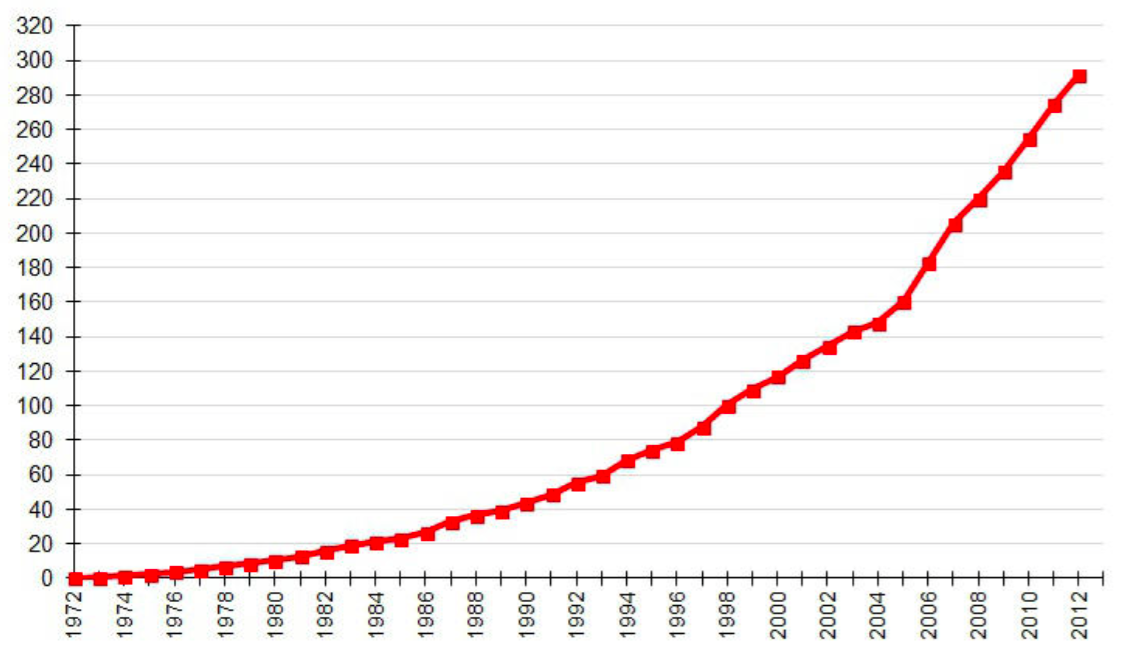
\includegraphics[width=0.95\textwidth]{figure/volumetria_teleriscaldata} 
\caption{Andamento della volumetria teleriscaldata in Italia dal 1972 al 2012 in Milioni di $m^3$.}
\label{fig:volumetria_teleriscaldata}
\end{figure}

Come è possibile osservare nella Tabella \ref{tab:volumetrie_teleriscaldamento} la distribuzione territoriale degli impianti di teleriscaldamento in Italia, in termini di volumetria allacciata alle reti risulta concentrata nell'Italia settentrionale e la quasi totalità della volumetria teleriscaldata (circa 281 milioni di $m^3$, pari al 96\% della volumetria totale) è localizzata in quattro regioni, dove la Lombardia risulta avere il maggior volume riscaldato con 120 milioni di metri cubi e il 43\% del totale nazionale, seguita dal Piemonte e dall'Emilia Romagna, rispettivamente con 76 e 38 milioni di metri cubi serviti e dal Veneto con 14 milioni di metri cubi e il 5\% del totale.

\begin{table}[!ht]
\centering
\resizebox{\columnwidth}{!}{%
\begin{tabular}{|l|c|c|c|c|c|c|}
\hline
\multirow{2}{*}{\textbf{REGIONE}} & \multicolumn{1}{l|}{\textbf{Popolazione residente}} & \multicolumn{5}{c|}{\textbf{Volumetria riscaldata}}                                                                                                                                                         \\ \cline{2-7} 
                                  & \textit{N.}                                         & \multicolumn{1}{l|}{\textit{Mm}} & \multicolumn{1}{l|}{\textit{m/resid}} & \multicolumn{1}{l|}{\textit{Residenziale}} & \multicolumn{1}{l|}{\textit{Terziario}} & \multicolumn{1}{l|}{\textit{Industriale}} \\ \hline
Lombardia                         & 9.973.397                                           & 125                              & 13                                    & 69                                         & 53                                      & 3                                         \\ \hline
Piemonte                          & 4.436.798                                           & 76                               & 17                                    & 57                                         & 18                                      & 1                                         \\ \hline
Emilia Romagna                    & 4.446.354                                           & 38                               & 9                                     & 22                                         & 16                                      & 0                                         \\ \hline
Trentino                          & 989.109                                             & 27                               & 27                                    & 18                                         & 8                                       & 1                                         \\ \hline
Veneto                            & 4.926.818                                           & 14                               & 3                                     & 11                                         & 4                                       & 0                                         \\ \hline
Liguria                           & 1.591.939                                           & 4                                & 2                                     & 0,6                                        & 1,1                                     & 2,1                                       \\ \hline
Lazio                             & 5.870.451                                           & 3                                & 1                                     & 2,8                                        & 0,4                                     & 0                                         \\ \hline
Toscana                           & 3.750.511                                           & 2                                & 0                                     & 1,5                                        & 0,3                                     & 0                                         \\ \hline
Valle d'Aosta                     & 128.19                                              & 2                                & 12                                    & 0,8                                        & 0,7                                     & 0                                         \\ \hline
Marche                            & 1.553.138                                           & 1                                & 0                                     & 0,4                                        & 0,3                                     & 0                                         \\ \hline
\textbf{TOTALE}                   & \textbf{37.666.634}                                 & \textbf{292}                     & \textbf{85}                           & \textbf{182}                               & \textbf{102}                            & \textbf{8}                                \\ \hline
\end{tabular}}
\caption{Volumetrie allacciate al TLR in Italia.}
\label{tab:volumetrie_teleriscaldamento}
\end{table}

Prendendo in considerazione il rapporto tra i metri cubi riscaldati e la popolazione
residente, la Regione che offre le migliori prestazioni è il Trentino Alto Adige, seguita dal Piemonte e dalla Lombardia. 
Scendendo a livello locale è il Comune di Torino a presentare la maggior volumetria teleriscaldata con 53,4 milioni di $m^3$, seguito da Brescia $41,3$ e Milano con $30,7$ milioni di $m^3$.\\

%\subsubsection{Estensione delle reti e numero di sottocentrali d'utenza}
L'estensione delle reti di riscaldamento urbano in Italia ha raggiunto, nel 2012, i 3.663 km di rete primaria (stacchi d'utenza esclusi), pari a poco meno di 3,5 volte l'estensione nell'anno 2000.
Le reti di teleriscaldamento si suddividono in tre categorie: le reti ad acqua calda, tecnologia un tempo riservata alle piccole e medie estensioni ma oggi applicata anche alle reti di dimensioni maggiori, rappresentano ormai la tipologia prevalente; la restante quota è costituita da reti ad acqua surriscaldata e da reti a vapore, tecnologia presente solo nelle reti geotermiche della Toscana.\\

Sono invece 66.887 gli impianti d'utenza presenti in Italia. Di questi 19.841 per solo riscaldamento e 47.046 per riscaldamento e
produzione di acqua calda sanitaria. \`E la Lombardia la Regione con il maggior numero di sottostazioni di utenza (SST), seguita dal Trentino Alto Adige e dal Piemonte. Maggiori informazioni sono visibili nella Tabella \ref{tab:rete_italia}.

% Please add the following required packages to your document preamble:
% \usepackage{multirow}
\begin{table}[!ht]
\centering
\resizebox{\columnwidth}{!}} \\ \cline{2-4}
                                  & \textit{N.}     & \multicolumn{2}{c|}{\textit{Abitanti equivalenti}}                           &                              \\ \hline
Lombardia                         & 29.829          & 8.723.867                    & 1.249.530                                     & 12,5                         \\ \hline
Piemonte                          & 8.813           & 3.673.261                    & 763.537                                       & 17,5                         \\ \hline
Emilia Romagna                    & 6.126           & 4.061.475                    & 384.879                                       & 8,66                         \\ \hline
Trentino                          & 16.099          & 721.190                      & 267.919                                       & 27,1                         \\ \hline
Veneto                            & 1.896           & 4.783.794                    & 143.024                                       & 2,9                          \\ \hline
Liguria                           & 71              & 1.554.044                    & 37.895                                        & 2,38                         \\ \hline
Lazio                             & 402             & 5.838.057                    & 32.394                                        & 0,55                         \\ \hline
Toscana                           & 2879            & 3.732.793                    & 17.718                                        & 0,47                         \\ \hline
Valle d'Aosta                     & 368             & 112.279                      & 15.840                                        & 12,4                         \\ \hline
Marche                            & 404             & 1.546.492                    & 6.646                                         & 0,43                         \\ \hline
\textbf{TOTALE}                   & \textbf{66.887} & \textbf{34.747.252}          & \textbf{2.919.382}                            & \textbf{7,75}                \\ \hline
\end{tabular}}
\caption{Diffusione delle sottostazioni di utenza e numero di abitanti equivalenti serviti da TLR nelle regioni italiane.}
\label{tab:rete_italia}
\end{table}


Le reti di teleriscaldamento in esercizio in Italia hanno erogato all'utenza circa 8.394 GWht, di cui la quota prevalente pari a 4.054 GWht, il 48\% del totale, è prodotta tramite impianti cogenerativi alimentati da fonti fossili (costituite, queste, per la quasi totalità da gas). La restante quota è suddivisa equamente tra fonti di energia rinnovabili (2.151 GWht con il 26\%) e caldaie a combustibili fossili (2.189 GWht, 26\%). Si veda la Figura \ref{fig:torta}.

\begin{figure}[!ht]
\centering
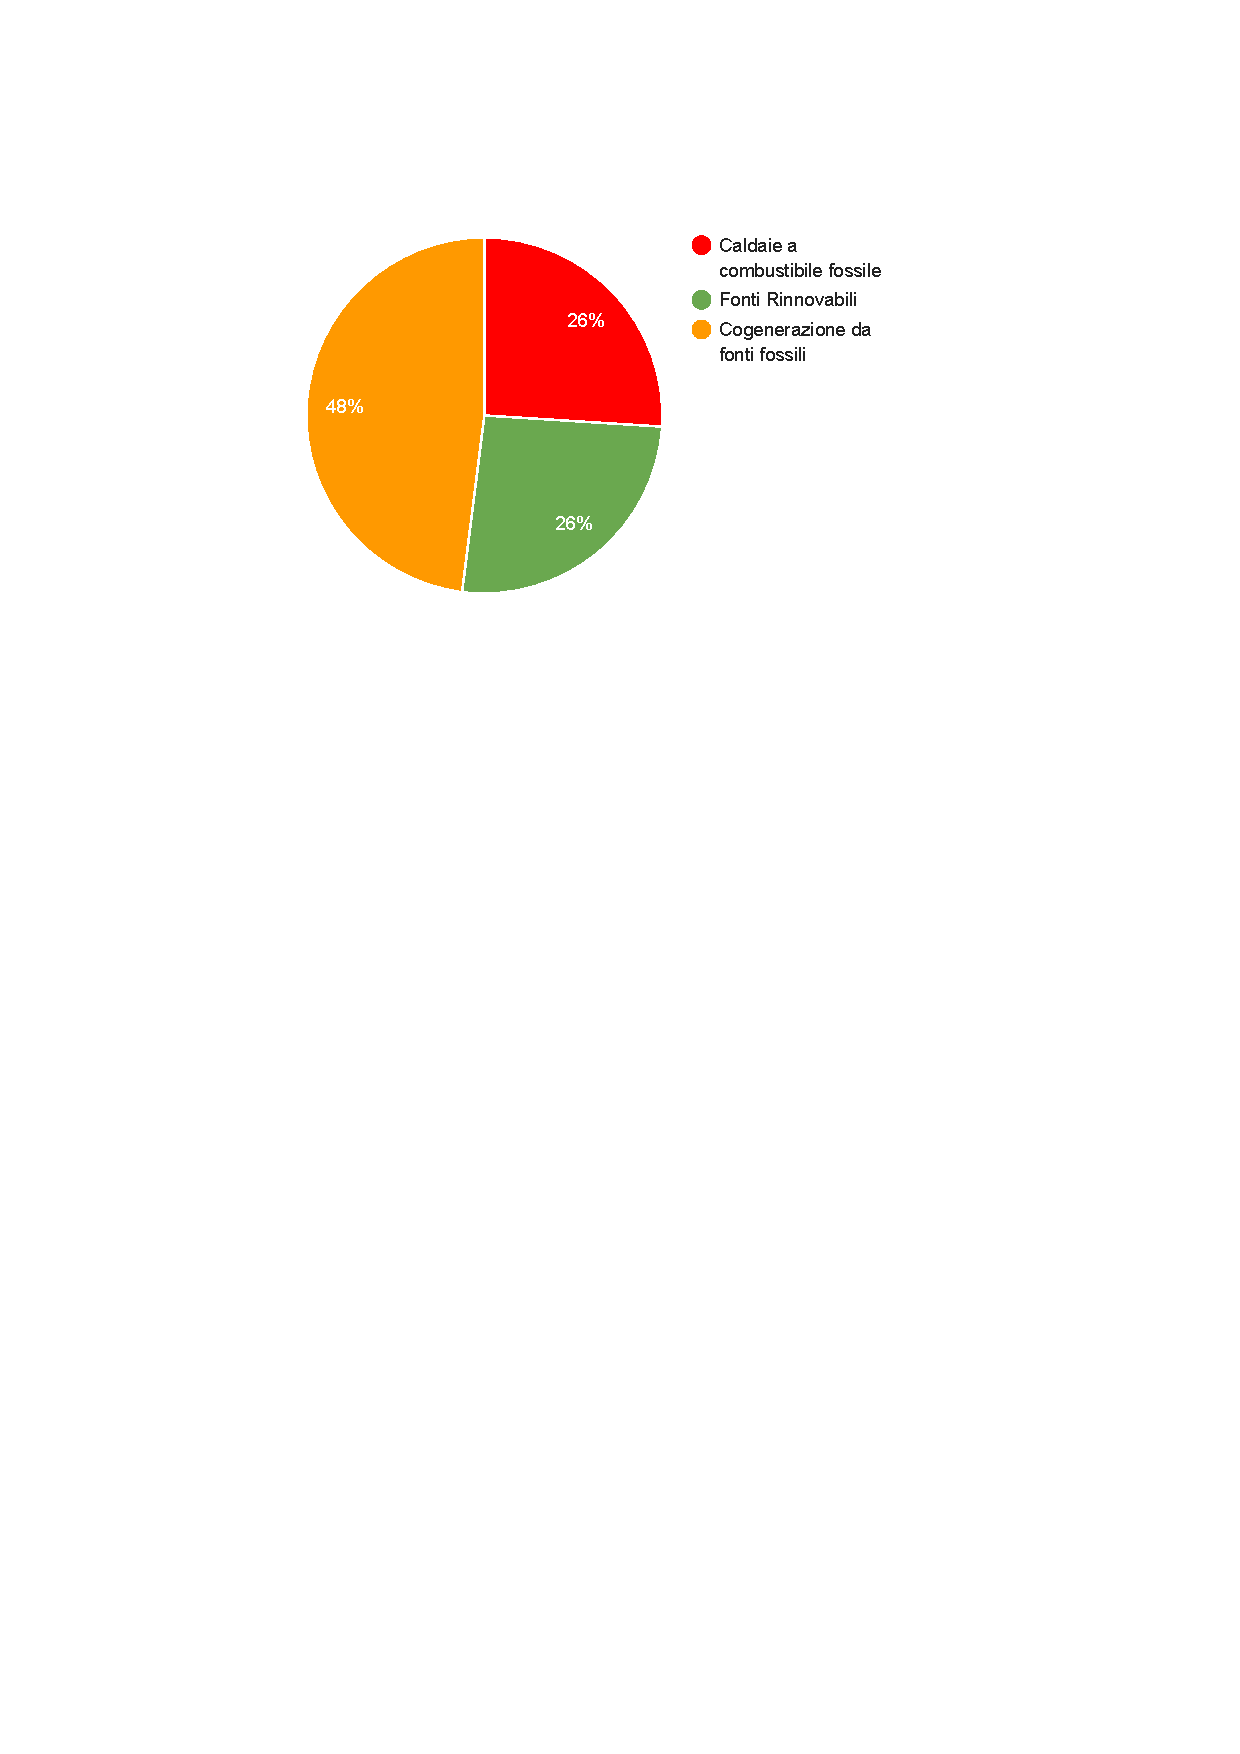
\includegraphics[width=0.75\textwidth]{figure/torta_energia} 
\caption{Provenienza dell'energia termica erogata all'utenza in generale.}
\label{fig:torta}
\end{figure}

Come ben si nota, la maggior parte di energia risulta prodotta da combustibili di tipo fossile che sono presenti sopratutto in Lombardia e Piemonte.
Nel grafico della Figura \ref{fig:energia_green} è rappresenta la quantità di energia termica erogata all'utenza prodotta tramite fonti ''green'', intendendo, convenzionalmente come tale, l'energia prodotta tramite impianti di cogenerazione, tramite fonti rinnovabili vere e proprie (biomassa e geotermia), tramite pompe di calore e tramite recupero di energie altrimenti disperse (in questa categoria è inclusa la termo-distruzione dei rifiuti solidi urbani).
Risulta che in ben cinque Regioni tale quota supera il 75\%, qualificando le rispettive reti (a livello complessivo) come "teleriscaldamento efficiente" come definito dai recentissimi orientamenti legislativi (Legge n. 164 del 11 novembre 2014).
La situazione nelle restanti regioni evidenzia un minore utilizzo degli impianti "green" installati.

\begin{figure}[!ht]
\centering
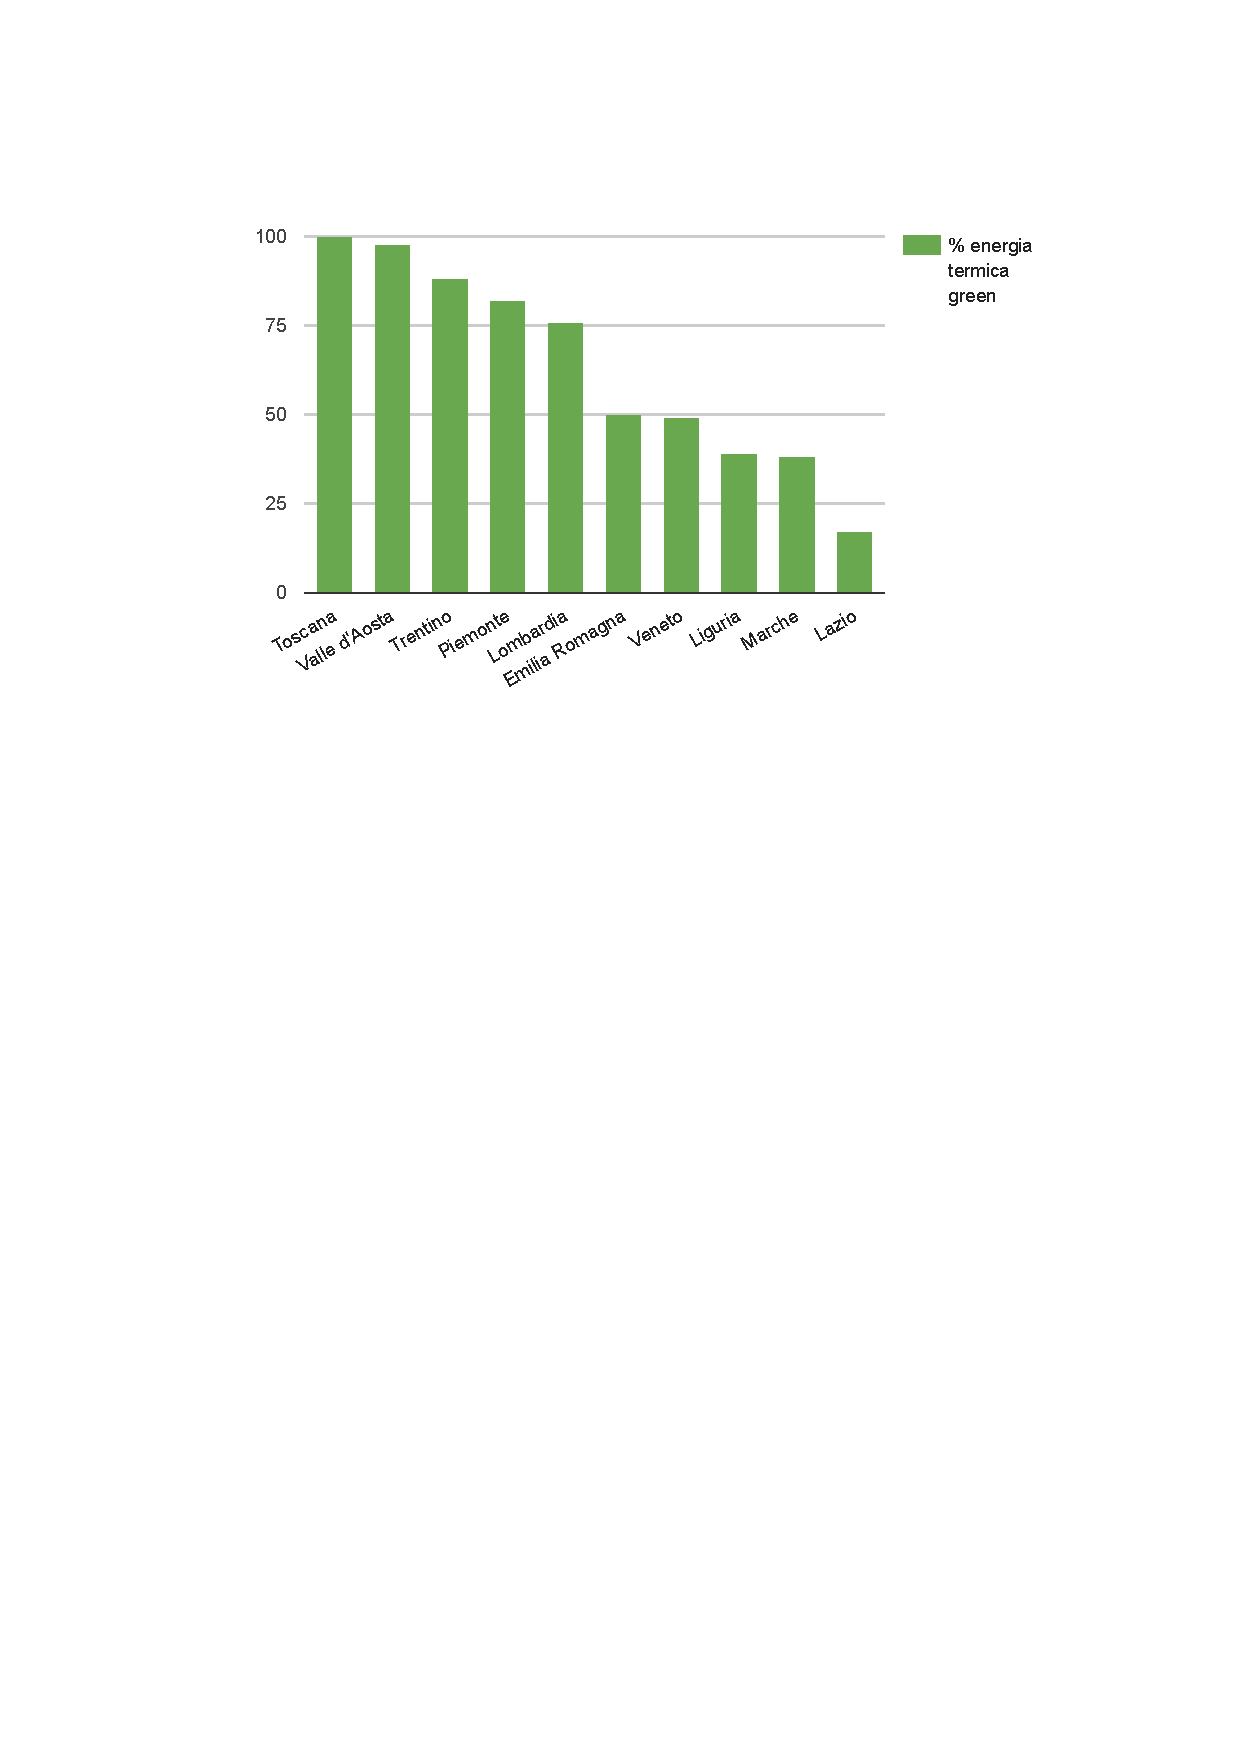
\includegraphics[width=\textwidth]{figure/energia_green} 
\caption{Provenienza dell'energia termica erogata all'utenza in generale.}
\label{fig:energia_green}
\end{figure}

Per comprendere l'efficienza delle reti di teleriscaldamento è necessario studiare e comprendere due parametri fondamenti, il risparmio dell'energia primaria e il conseguente risparmio di anidride carbonica immessa in atmosfera rispetto all'utilizzo di sistemi di riscaldamento tradizionali individuali alimentati a gas. Il risparmio dell'energia primaria quindi vuol dire non solo più efficienza in termini di copertura dei fabbisogni ma anche minori importazioni di combustibili fossili esteri e quindi in un risparmio anche economico. Nel 2012 i sistemi di riscaldamento urbano operanti in Italia hanno conseguito un risparmio di energia primaria fossile di circa 478.000 TEP, corrispondente a circa il 25\% dell'energia consumata dai "sistemi convenzionali sostituiti" (caldaie di edificio e sistema elettrico nazionale). Di tale risparmio, ben il 91\% è realizzato in sole tre regioni (Piemonte, Lombardia e Trentino A. A.) (si veda Figura \ref{fig:tep}). 
Un altro importante contributo è arrivato inoltre dalle reti di teleriscaldamento toscane con il 92,9\% di energia primaria risparmiata a livello regionale e della Valle d'Aosta con l'85,1\%.

\begin{figure}[!ht]
\centering
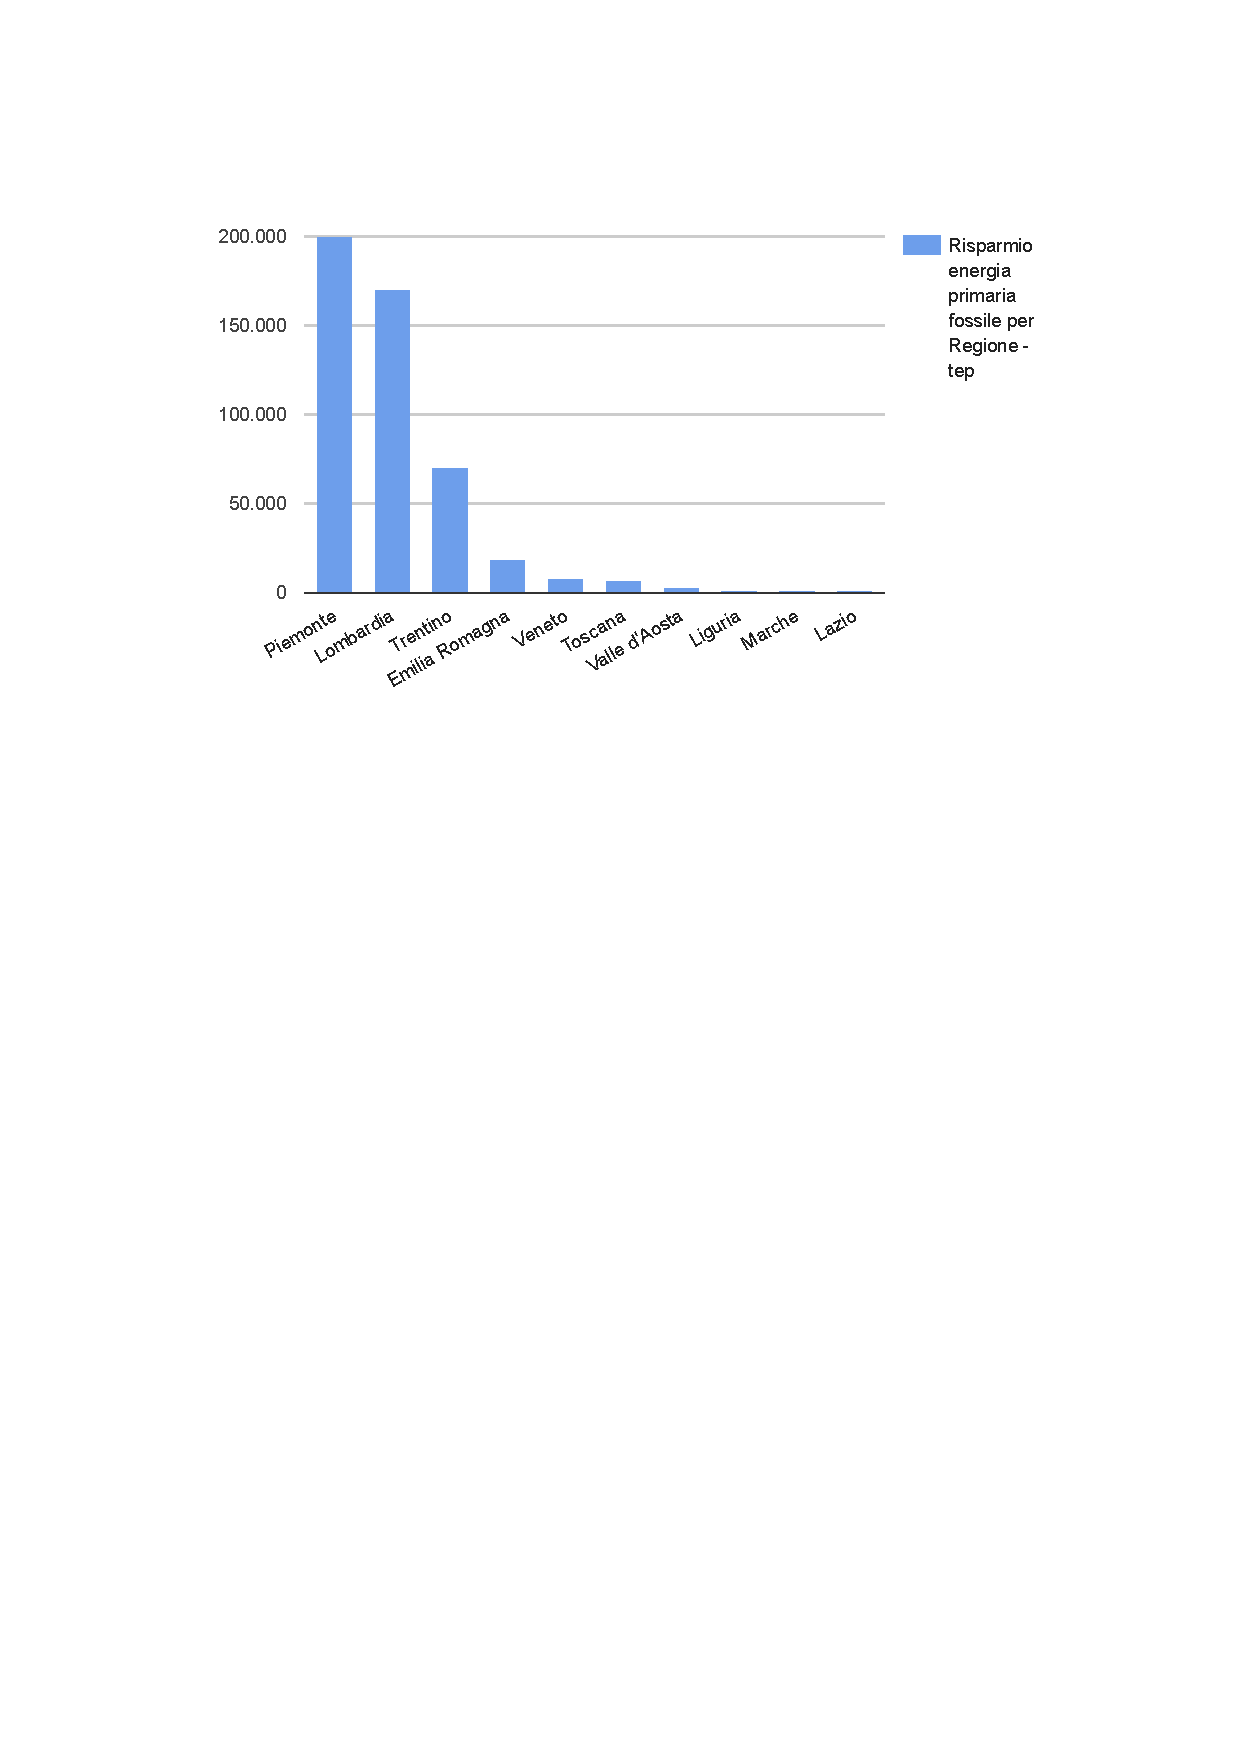
\includegraphics[width=\textwidth]{figure/tep} 
\caption{Risparmio di energia primaria fossile per regione - TEP.}
\label{fig:tep}
\end{figure}

Il risparmio di energia primaria oltre ad una riduzione dei costi nell'uso dei carburanti e un miglioramento della qualità dell'aria, si traduce, nel caso di sistemi efficienti, anche in emissioni evitate di CO$_2$.
Elevate prestazioni, in termini di emissioni di anidride carbonica evitate, vengono raggiunte dalle reti alimentate da impianti a fonti rinnovabili, come nel caso della Valle d'Aosta, del Trentino Alto Adige e della Toscana visibili in Figura \ref{fig:CO2}. Quest'ultima in particolare ha ridotto le emissioni di circa il 90\%.

\begin{figure}[!ht]
\centering
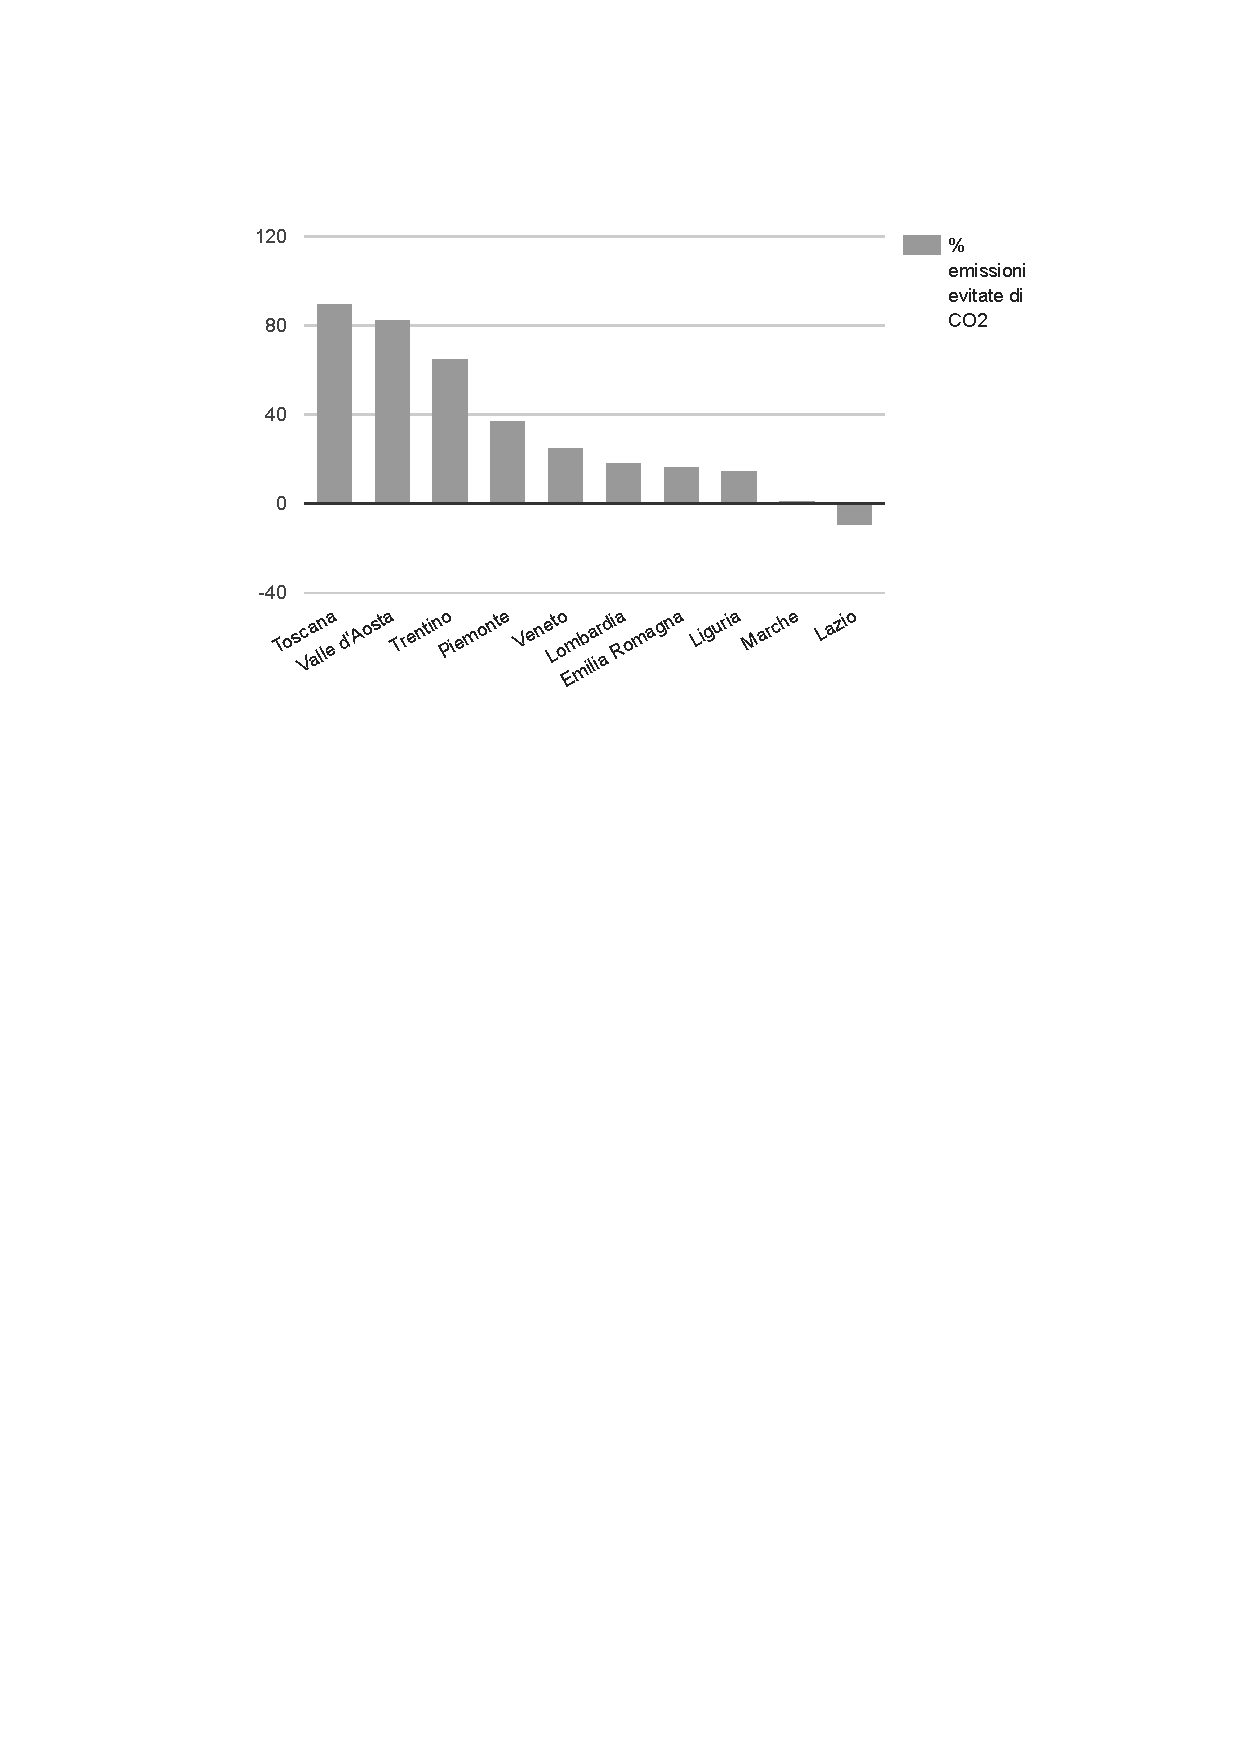
\includegraphics[width=\textwidth]{figure/CO2} 
\caption{Percentuale di emissioni di CO$_2$ evitate dagli impianti di TLR per regione.}
\label{fig:CO2}
\end{figure}

Non possiamo sottacere i casi che presentano problematiche: le reti di teleriscaldamento delle regioni Marche e Lazio non producono benefici ambientali.\\

I dati del teleriscaldamento in Italia appaiono assai più interessanti se si considera quanta strada ancora si potrebbe fare nel nostro Paese in termini di sviluppo di questa tecnologia. Sono oltre 5.300 i Comuni in cui è possibile realizzare impianti di teleriscaldamento, ovvero tutti quelli compresi nelle fasce climatiche E ed F, pari al 66\% del totale dei Comuni italiani. E di questi il 14\% non risulta raggiunta dalla rete di distribuzione del gas metano. 
Un'importante e confortante conclusione: lo sviluppo del teleriscaldamento in Italia è ancora ben lontano dalla saturazione.
Giova peraltro evidenziare le differenze, notevoli e giustificate dalle rispettive condizioni climatiche, per aree geografiche.\\

Regioni del Nord Italia: in queste regioni è localizzato il 62\% del potenziale tele riscaldabile. Il 30\% circa del potenziale risulta teleriscaldato. \\

Regioni del Centro Italia: in queste regioni è localizzato il 27\% del potenziale tele riscaldabile ma Solo l'1\% circa di tale potenziale risulta teleriscaldato. \\

Regioni del Sud Italia: In queste regioni è localizzato l'11\% del potenziale teleriscaldabile. In tale area non esistono ad oggi reti di teleriscaldamento.

\section{Le rinnovabili termiche: energia geotermica}
Spesso si confonde il fabbisogno di energia con il fabbisogno di energia elettrica. E i maggiori consumi di energia non sono quelli elettrici, ma quelli termici. Il settore delle "rinnovabili termiche", ossia tutte le tecnologie per il riscaldamento e il raffrescamento alimentate con fonti rinnovabili è sempre più studiato  al fine di ridurre l'inquinamento dovuto ai combustibili fossili.
Produrre calore senza inquinare e dimezzando i consumi elettrici, oggi è possibile grazie all'energia accumulata nel suolo, ovvero la cosiddetta energia geotermica.\\

Per energia geotermica si intende l'energia contenuta sotto forma  di calore nell'interno della Terra; l'origine di questo calore è in relazione con la natura interna del nostro pianeta. Malgrado tale calore sia in quantità enorme e praticamente inesauribile, anche considerando solo la crosta terrestre e non le zone più profonde del pianeta, esso è tuttavia assai disperso, raramente concentrato e situato a profondità troppo elevate per essere sfruttato industrialmente. Il calore interno si dissipa con continuità verso la superficie della terra, ma i suoi effetti sono in genere poco percettibili. La temperatura delle rocce aumenta progressivamente con la profondità in media di $3 ^{\circ }C$ ogni 100 metri ($30 ^{\circ} C/km$), questo aumento è chiamato gradiente termico.

Esistono tuttavia nella crosta terrestre, a profondità accessibili ai nostri mezzi (1-4 km) delle zone privilegiate, ove il gradiente è nettamente superiore a quello medio. Ciò è dovuto in certi casi alla presenza, non lontano dalla superficie (5-10 km), di masse magmatiche fluide o già solidificate in via di raffreddamento. In altri casi, in aree non interessate direttamente da attività magmatica, l'accumulo di calore è dovuto a particolari situazioni idrogeologiche della crosta terrestre.

I fluidi geotermici presenti nella crosta terrestre sono formati prevalentemente da acqua originariamente meteorica, penetrata nel sottosuolo nel corso di centinaia di migliaia di anni e che si è riscaldata a contatto delle rocce calde e permeabili. Queste rocce formano degli acquiferi caldi, detti serbatoi geotermici, che possono raggiungere anche temperature elevate oltre i 300 $^{\circ}C$. In condizioni ottimali gli acquiferi geotermici, oltre all'acqua in fase liquida, possono contenere come prevalente la fase vapore che ovviamente possiede un contenuto energetico assai più elevato.

Spesso i fluidi caldi rimangono confinati entro il serbatoio per effetto di una copertura di terreni impermeabili. In tal caso possono essere estratti tramite pozzi profondi fino a qualche chilometro, mettendo così in comunicazione diretta la risorsa geotermica con la superficie per il successivo utilizzo energetico del calore. 

Il calore estratto può essere utilizzato oltre che per la produzione di energia elettrica come fonte termica per alimentare impianti di teleriscaldamento.

Le sorgenti geotermiche possono essere classificate in 4 differenti tipologie:
\begin{itemize}
\item alta entalpia: presenza di vapore oltre i 150 $^{\circ}C$ utilizzato principalmente per la produzione di energia nobile (elettrica). Questa risorsa è territorialmente localizzata e comporta alti investimenti per il suo sfruttamento;
\item media Entalpia: presenza di acqua calda tra i 50 ei 150 $^{\circ}C$che non può essere utilizzata per la produzione di energia elettrica ma può essere usata per fornire calore.;
\item bassa entalpia: presenza di acqua calda sotto i 50 $^{\circ}C$ che come nel caso precedente può essere sfruttata soltanto per la produzione di acqua calda;
\item terreno: viene sfruttato lo scambio termico con il sottosuolo superficiale, per mezzo di una pompa di calore. Il suolo rappresenta per la pompa di calore una sorgente di calore. Rispetto all'aria atmosferica, che è la sorgente adoperata dalle pompe di calore aerotermiche, la temperatura del suolo ad una certa profondità subisce variazioni annuali molto più contenute: a profondità di 5-10 metri la temperatura del suolo è pressoché costante tutto l'anno ed è equivalente all'incirca alla temperatura media annuale dell'aria, ovvero circa 10-16 $^{\circ}C$. Ciò significa che il suolo, rispetto all'aria, è più caldo d'inverno e più fresco d'estate, a vantaggio del rendimento della pompa di calore.
\end{itemize}


\section{La geotermia per il riscaldamento: il caso Toscana}
Uno dei primi esempi di teleriscaldamento in Italia è quello di Larderello (PI) del 1960, a margine della produzione di energia elettrica da fonte geotermica ENEL. È rimasto per lungo tempo il principale esempio di teleriscaldamento alimentato da fonte geotermica in Italia.
In seguito l'utilizzo diretto dell'energia si è diffuso negli altri paesi toscani a partire dalla metà degli anni 80: 
\begin{itemize}
\item 1960: Teleriscaldamento Villaggio di Larderello
(ENEL)
\item 1985: Teleriscaldamento comune di Castelnuovo Val di Cecina
\item 1993 – 1995: Costruzione e avviamento teleriscaldamento di Lustignano, Serrazzano, Montecerboli, Larderello (fuori villaggio ENEL)
\item 1998–2000:costruzione e avviamento teleriscaldamento di San Dalmazio
\item 2000 – 2002: Costruzione e avviamento del teleriscaldamento di Pomarance
\item Dal 2000 : Costruzione e avviamento del teleriscaldamento di Santa Fiora (m.te Amiata)
\item Altre estensioni ed evoluzioni
\end{itemize}

I Teleriscaldamenti nell'area tradizionale toscana sono esempi di utilizzo diretto da sorgente geotermica ad alta entalpia (vapore). La principale difficoltà nella realizzazione di questi impianti sono i costi elevati di costruzione. I vantaggi che però determina una rete teleriscaldata riguardano: il comfort climatico dell'abitazione; il rispetto per l'ambiente riducendo a zero le emissioni di CO$_2$; la sicurezza e l'economicità per l'utente. 

In Toscana non ci sono (al momento) impianti di grandi dimensioni.

I primi esempi, a seguito di quello di Larderello, si sono avuti nelle aree dove c'è disponibilità di fonti di calore conosciute.
Questo spiega la diffusione principalmente nell'area geotermica tradizionale ad alta entalpia, come visibile in Figura \ref{fig:toscana}.

\begin{figure}[!ht]
\centering
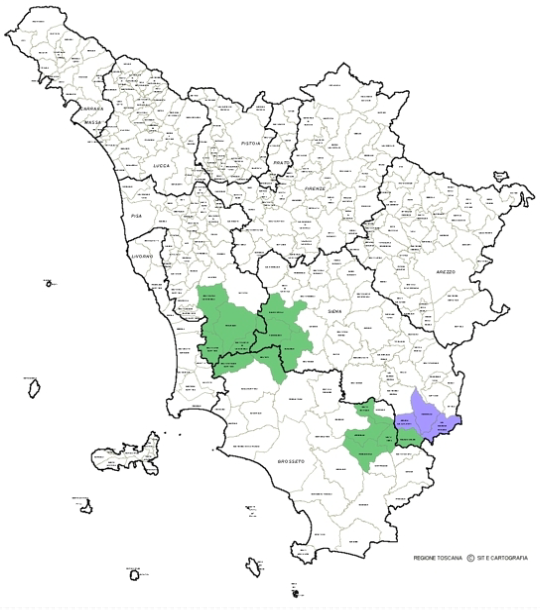
\includegraphics[width=0.8\textwidth]{figure/toscana}
\caption{Le zone evidenziate rappresentano i luoghi della regione Toscana dove si utilizzano impianti di teleriscaldamento alimentati da fonte di calore geotermica.}
\label{fig:toscana}
\end{figure}

Gli impianti di teleriscaldamento operativi in queste zone alimentano  piccoli/medi centri abitati utilizzando quindi impianti medio/piccoli, economicamente sostenibili con modelli di progettazione esportabili indipendentemente dalla fonte utilizzata. Le reti toscane presenti sono descritte nella Tabella \ref{tab:reti_toscane}.

% Please add the following required packages to your document preamble:
% \usepackage{multirow}
\begin{table}[]
\centering
\resizebox{\columnwidth}{!}{%
\begin{tabular}{|l|c|c|c|}
\hline
\textbf{Comune}                                                                           & \textbf{Reti presenti} & \textbf{\begin{tabular}[c]{@{}c@{}}Anno di inizio esercizio\\ o stato dell'arte\end{tabular}}       & \textbf{Utenze complessive}  \\ \hline
\multirow{6}{*}{Pomarance (PI)}                                                           & Capoluogo              & 2002                                                                                                & \multirow{6}{*}{2.600}       \\ \cline{2-3}
                                                                                          & Larderello             & 1955                                                                                                &                              \\ \cline{2-3}
                                                                                          & Montecerboli           & 1996                                                                                                &                              \\ \cline{2-3}
                                                                                          & Lustignano             & 1998                                                                                                &                              \\ \cline{2-3}
                                                                                          & Serrazzano             & 1998                                                                                                &                              \\ \cline{2-3}
                                                                                          & San Dalmazio           & 2002                                                                                                &                              \\ \hline
\multirow{3}{*}{\begin{tabular}[c]{@{}l@{}}Castelnuovo\\ Val di Cecina (PI)\end{tabular}} & Capoluogo              & 1985                                                                                                & \multirow{3}{*}{1.099}       \\ \cline{2-3}
                                                                                          & Sasso Pisano           & 1995                                                                                                &                              \\ \cline{2-3}
                                                                                          & Montecastelli          & 2009                                                                                                &                              \\ \hline
\begin{tabular}[c]{@{}l@{}}Monterotondo\\ Marittimo (GR)\end{tabular}                     & -                      & 1996                                                                                                & 399                          \\ \hline
Santa Fiora (GR)                                                                          & -                      & 2005                                                                                                & 840                          \\ \hline
\multirow{2}{*}{\begin{tabular}[c]{@{}l@{}}Monteverdi\\ Marittimo (PI)\end{tabular}}      & Capoluogo              & \multirow{2}{*}{\begin{tabular}[c]{@{}c@{}}prima parte: 2013 \\ completamento: 2014\end{tabular}} & \multirow{2}{*}{204}         \\ \cline{2-2}
                                                                                          & Canneto                &                                                                                                     &                              \\ \hline
Montieri (GR)                                                                             & -                      & 2014                                                                                                & 425                          \\ \hline
\multirow{2}{*}{Radicondoli (SI)}                                                         & Capoluogo              & \multirow{2}{*}{2016}                                                                               & \multirow{2}{*}{847 (Stima)} \\ \cline{2-2}
                                                                                          & Belforte               &                                                                                                     &                              \\ \hline
Chiusdino (SI)                                                                            & -                      & \begin{tabular}[c]{@{}c@{}}completamento previsto\\ 2017\end{tabular}                               & 387 (Stima)                  \\ \hline
\end{tabular}}
\caption{Reti toscane di teleriscaldamento geotermico in funzione, in corso di realizzazione ed in fase di gara.}
\label{tab:reti_toscane}
\end{table} 

 Nel resto della Toscana si sono recentemente realizzati impianti a biomassa (da 300 KWt a 1500 KWt), dove la risorsa è più facilmente disponibile (Garfagnana, Appennino).
 

\section{Geo Energy Service e criticità degli impianti}
Nel comune di Pomarance, l'azienda Geo Energy Service s.p.a. (G.E.S. s.p.a.), nata nel luglio del 2006, si occupa della gestione delle centrali termiche e delle relative reti di teleriscaldamento nell'area geotermica tradizionale della Toscana. Gli impianti di teleriscaldamento gestiti sono alimentati ad energia geotermica ad alta entalpia (vapore surriscaldato). Negli ultimi anni vi sono stati ampli ammodernamenti tecnologici al fine di migliorare l'efficienza degli impianti e di conseguenza il livello di servizio agli utenti, pur mantenendo l'economicità del servizio. La rete di teleriscaldamento, con oltre 80 km di estensione totale, si è particolarmente ampliata negli anni con impianti anche nelle zone extraurbane che servono diverse strutture turistiche , fornendo la possibilità di lavorare a tariffe competitive anche in inverno. I lavori di estensione e di continuo aggiornamento degli impianti consentono positive ricadute sull'economia della zona e sulle professionalità presenti sul territorio, anche sperimentando utilizzi industriali diretti dell'energia geotermica (forni di verniciatura, essiccazione, lavanderie, processi industriali etc..).  

La GES ha attualmente la gestione di 7 reti di teleriscaldamento geotermiche e di una a biomassa nell'area geotermica tradizionale, inoltre ha esperienza in impianti fotovoltaici integrati, ed ha in corso lavori per l'allacciamento di ulteriori 130.000 $m^3$ di utenze, utilizzando energia geotermica. Un altro interessante progetto prevede l'integrazione dell'impianto alimentato a biomassa e di uno alimentato con energia geotermica e con energia solare. Il progetto è sviluppato nell'ambito del Solar District heating Project, al quale partecipiamo come stake holders italiani insieme ad HERA attraverso AIRU (Associazione Italiana Riscaldamento urbano).
In sintesi:
\begin{itemize}
\item Volumetria utenze attive: 782.656 $m^3$
\item Numero utenze attive: 2263
\item Lunghezza rete 80 Km (doppio tubo)
\item 45000 Gcalh/anno erogati; 
\item 4.200 TEP risparmiate (29.000 barili di petrolio) ovvero 13.000 ton di CO2/anno non emessa
\end{itemize}

%Nel comune di Pomarance, l'azienda Geo Energy Service s.p.a. (G.E.S. s.p.a.), nata nel luglio del 2006, si occupa della gestione delle centrali termiche e delle relative reti di teleriscaldamento. L'azienda è situata nella provincia di Pisa storicamente importante per lo sviluppo e lo sfruttamento dell'energia geotermica, sopratutto nella frazione di Larderello. La società in totale gestisce nove centrali termiche alimentate da energia geotermica e sei reti di teleriscaldamento che si estendono per 200 km, per un totale di $2.400$ utenze con una volumetria di circa $800.000 \ m^3$, erogando energia per circa $45.000 \ Gcal/anno$ che evita il consumo di 4132 TEP/anno. 

Grazie alla collaborazione con ENEL per la ricerca di sorgenti di vapore non idonee per la produzione di energia elettrica, l'azienda può  mantenere tariffe economiche in quanto può avere accesso ad una fonte di energia termica praticamente a costo zero. Non per questo si ha che le i costi di gestione degli impianti siamo bassi. Il trasporto di acqua calda ai centri abitativi è reso possibile per mezzo di grosse stazioni di pompaggio e proprio queste sono le responsabili delle maggiori spese di gestione di un impianto. 

Dato che uno dei principali obiettivi del teleriscaldamento è fornire un certo livello di comfort all'utenza ad un prezzo vantaggioso è necessario che i costi dovuti all'energia di pompaggio vengano ridotti al minimo introducendo opportune regolazioni e sistemi di controllo ottimizzati. 

L'azienda è motivata a raggiungere tale obiettivo e perciò ha richiesto la collaborazione con l'università degli studi di Siena per analizzare i vantaggi applicabili alle reti già esistenti.

Il problema che riguarda le ingenti spese di energia elettrica per la circolazione di acqua calda è maggiormente visibile in impianti dove il costo del calore è irrisorio (come nel caso della fonte geotermica) ma influisce molto anche in impianti che producono energia termica grazie alla cogenerazione o altre fonti rinnovabili. Detto ciò i sistemi che verranno studiati potranno essere esportati a qualsiasi tipo di impianto di teleriscaldamento.


\chapter{Tecnologie degli impianti di teleriscaldamento}
%\label{Capitolo3}
Un impianto di teleriscaldamento è un  sistema di riscaldamento a distanza di un quartiere o di una città 
che utilizza il calore prodotto da una centrale termica, da un impianto di cogenerazione o da una sorgente geotermica, distribuendolo agli edifici tramite una rete di tubazioni in cui fluisce l'acqua calda che verrà utilizzata per la produzione di acqua igienico sanitaria e il riscaldamento di edifici residenziali e commerciali. Indipendentemente dal tipo di fonte di calore usata per la produzione di energia termica, la struttura e gli elementi principali di un impianto di teleriscaldamento rimangono invariati, come anche le problematiche relative all'ottimizzazione dei costi di gestione. In questa tesi, ci si concentra su impianti alimentati da fonte di calore geotermica. In questo tipo di impianto il pompaggio dell'acqua è responsabile di una significante parte del consumo totale di energia elettrica. Risulta quindi di interesse ridurre il più possibile questi consumi, tramite un'analisi degli aspetti che influenzano maggiormente il fenomeno e delle possibili azioni correttive. 

\section{Struttura di un impianto}
Le componenti principali di un sistema di teleriscaldamento sono  riportate in Figura \ref{fig:schema1}: una centrale termica, dove viene prodotto il calore, una rete di distribuzione, costituita da tubazioni 
coibentate interrate, e un insieme di sotto-centrali. Queste ultime, situate nei singoli 
edifici da servire, sono costituite da scambiatori di calore, che permettono di realizzare 
lo scambio termico tra il fluido termovettore  della rete primaria di teleriscaldamento e l'acqua del circuito delle utenze, senza che vi sia così miscelazione tra i due fluidi e  semplificando quindi notevolmente la progettazione dell'intera rete. Lo scambiatore, infatti, andrà semplicemente a sostituire la  caldaia convenzionale mantenendo invariato l'impianto già esistente dell'utenza.

\begin{figure}[!ht]
\centering
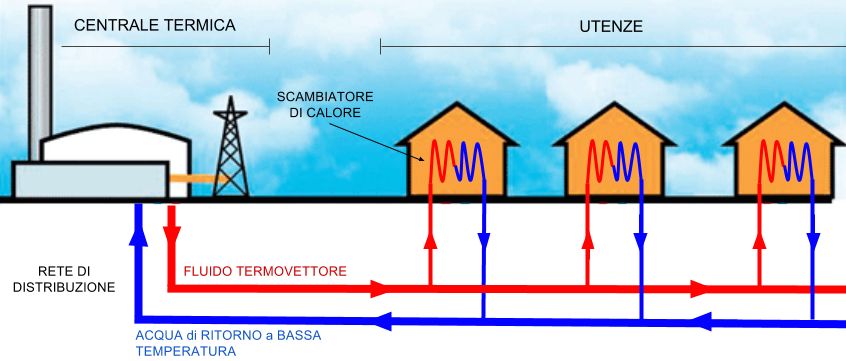
\includegraphics[width=1.0\textwidth]{figure/schema_impianto1}
\caption{Schema di un impianto di teleriscaldamento composto da centrale di scambio, rete di distribuzione e sotto-centrali di scambio (scambiatori).}
\label{fig:schema1}
\end{figure}

La centrale termica riscalda l'acqua che viene distribuita ai diversi edifici attraverso la rete di distribuzione con l'ausilio di pompe. Giunta allo scambiatore, l'acqua della rete trasferisce all'acqua dell'impianto di distribuzione interno dell'edificio, il calore necessario per riscaldare gli ambienti e per la produzione di acqua calda sanitaria. L'acqua, ormai raffreddata, ritorna in centrale per essere nuovamente riscaldata. 
%Il teleriscaldamento riesce ad essere economicamente conveniente a patto che si riesca a trovare un bacino di utenze concentrate in un'area relativamente ridotta. La traduzione inglese di teleriscaldamento "district heating" che letteralmente tradotta vuol dire "riscaldamento distrettuale", rende l'idea della concentrazione che l'utenza dovrebbe avere per far sì che questo metodo sia economicamente vantaggioso. \\
Nel seguito si analizza più approfonditamente ogni elemento dell'impianto.

\subsection{Centrale termica e di scambio}
Le centrali termiche, considerate in questa tesi, sfruttano il vapore geotermico non idoneo alla generazione di energia elettrica. Le centrali di scambio si occupano dello scambio di calore tra due diversi circuiti. La centrale termica può essere interpretata come una centrale di scambio in quanto non fa altro che estrarre dal vapore l'energia termica da scambiare con l'intero impianto di teleriscaldamento. Il vapore, dunque, arriva in centrale a circa $240 ^{\circ}$C e cede la sua energia termica attraverso gruppi di scambio termico costituiti da uno scambiatore vapore-acqua surriscaldata a circa $120 ^{\circ}$C e da un desurriscaldatore di condensa acqua. La portata del vapore è controllata attraverso  valvole a due vie di tipo NC (Normalmente Chiuse), in funzione della temperatura  di uscita dell'acqua surriscaldata desiderata nel circuito primario. La condensa viene raccolta in un serbatoio atmosferico e reiniettata nel punto di raccolta con pompe centrifughe multistadio, in modo da mantenere e rinnovare la risorsa geotermica. L'acqua surriscaldata viene inviata attraverso una linea feeder a una seconda centrale di scambio, posta nei pressi del centro abitativo, dove cede la sua energia termica attraverso gruppi di scambio termico costituiti da uno scambiatore acqua surriscaldata - acqua calda. La portata di acqua surriscaldata è controllata attraverso valvole a due vie di tipo NC, in funzione della temperatura in uscita dell'acqua calda nella rete di distribuzione. Questo ulteriore scambio permette di separare la linea dell'acqua surriscaldata  dai circuiti urbani, che sono più estesi, riducendo così la potenza dell'impianto di pompaggio, le perdite di calore e il costo della rete. Inoltre, l'utilizzo di acqua calda anziché surriscaldata nei centri urbani, aumenta il livello di sicurezza e riduce gli interventi di manutenzione dovuti alla maggiore complessità degli impianti di utenza ad acqua surriscaldata. La circolazione sia nel circuito primario che secondario sono garantite da elettropompe centrifughe ubicate nella stessa centrale di scambio (Figura \ref{fig:schema2}).
Nel caso in cui la centrale termica si trovi nei pressi delle utenze sarà possibile omettere la seconda centrale di scambio ed effettuare direttamente uno scambio di calore da vapore ad acqua calda (Figura \ref{fig:schema3}).

 \begin{figure}[!ht]
 \centering
 \subfigure[Schema di un impianto di teleriscaldamento con due centrali di scambio. Questa configurazione è utilizzata quando la centrale termica è distante dal centro abitativo.\label{fig:schema2}]
   {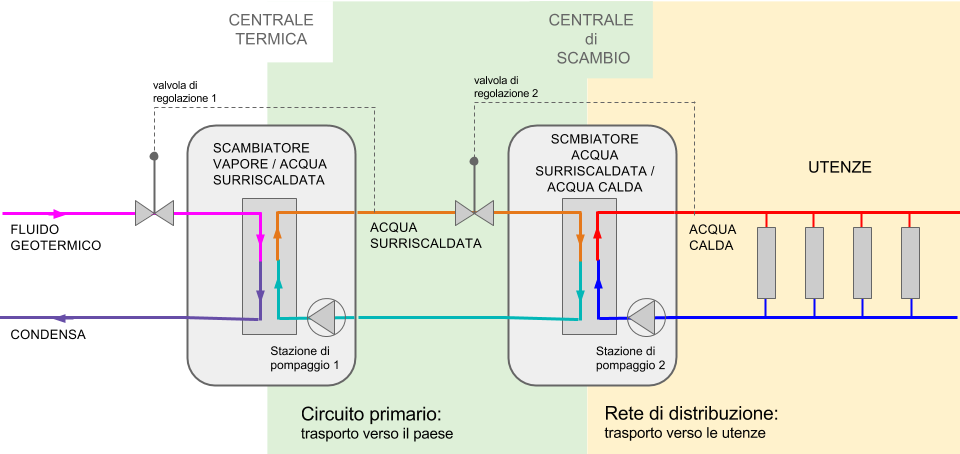
\includegraphics[width=12.5cm]{figure/schema_impianto2}}
 \hspace{5mm}
 \subfigure[Schema di un impianto di teleriscaldamento con singola centrale di scambio.\label{fig:schema3}]
   {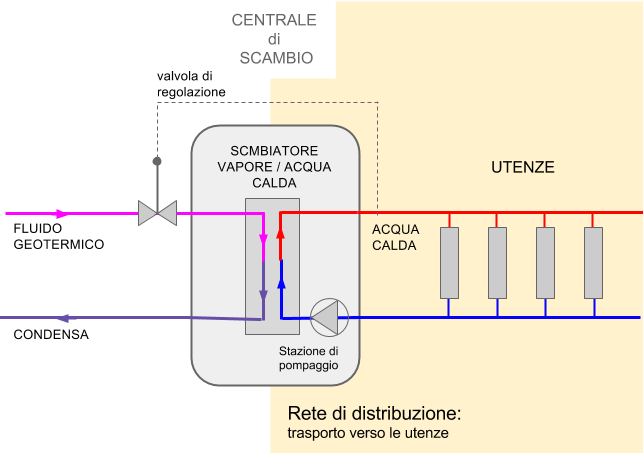
\includegraphics[width=8.5cm]{figure/schema_impianto3}}
 \caption{Possibili configurazioni di un impianto di teleriscaldamento alimentato da fonte geotermica.}
 \end{figure}

%lavorano a regime variabile 
\subsection{Stazioni di pompaggio}
Le stazioni di pompaggio si occupano del trasporto dell'acqua verso le sotto-centrali di scambio delle utenze.
I parametri di maggiore rilevanza che contraddistinguono le pompe sono la portata e la prevalenza:
\begin{itemize}
\item \textbf{Portata:} La portata della pompa è il volume d'acqua, misurato in litri o metri cubi, che viene mosso dalla pompa nell'unità di tempo (generalmente secondi o minuti). La portata si misura pertanto in litri al secondo ($l/sec$), litri al minuto ($l/min$), metri cubi all'ora ($m^3/h$), ecc.
\item \textbf{Prevalenza:} La prevalenza della pompa rappresenta l'incremento di energia acquisito da 1 $kg$ di liquido fra la sezione di entrata e quella di uscita della pompa stessa; generalmente si indica con $H$ e si misura in $J/kg$ oppure in metri ($m$) di liquido trasportato. Molto più comodo è parlare non di prevalenza bensì di prevalenza manometrica, indicata con $H_m$ e misurata in $m \ C.A.$ (metri di colonna d'acqua).
\end{itemize}

Le pompe solitamente usate sono pompe centrifughe, la cui curva caratteristica, in funzione della portata e della prevalenza, rimane abbastanza piatta per gran parte del range di portata. 
Il punto di funzionamento, ovvero la portata e la prevalenza realizzata delle pompe, dipende dalla resistenza offerta dalla rete dell'impianto. 
Le stazioni di pompaggio sono solitamente localizzate dentro la centrale di scambio e hanno il compito di assicurare un flusso di acqua tale da offrire ai complessi abitativi l'energia termica richiesta. Per di più, devono fornire alle utenze più sfavorite una differenza di pressione tale da garantire il passaggio di acqua all'interno dello scambiatore d'utenza. 
Quando la portata è elevata, le perdite di pressione nella rete aumentano e le pompe dovranno lavorare più duramente. La pressione sarà sempre sufficiente nelle sotto-stazioni vicine alla centrale, ma se la capacità limite della pompa viene raggiunta, la pressione nelle parti distanti della rete  può decadere impedendo agli scambiatori di calore di quelle zone di lavorare correttamente. I radiatori di queste utenze svantaggiate saranno freddi.

Come già citato, le pompe sono i principali elementi responsabili dei consumi di un impianto di teleriscaldamento, perciò è necessario introdurre delle regolazioni che limitino il più possibile gli sprechi di energia di pompaggio. Allo stesso tempo, si deve far si che in tutte le utenze sia garantita una differenza di pressione che permetta il corretto funzionamento degli scambiatori. 


%Le pompe solitamente usate sono pompe centrifughe, la cui curva caratteristica in funzione della portata e della prevalenza rimane abbastanza piatta per gran parte del range di portata. In base alla resistenza che offerta dalla rete la pompa lavorerà su uno specifico punto di funzionamento, il quale a sua volta è responsabile  
%Risulta dunque fondamentale avere una regolazione per evitare lo spreco di energia di pompaggio. 
%Nel caso vi siano due stazioni di pompaggio, e quindi due centrali di scambio, possiamo regolare  sia le pompe che alimentano il circuito primario che quelle della rete di distribuzione. Le pompe che alimentano il circuito primario sono regolate in base al grado di laminazione della valvola nella seconda centrale di scambio, la quale garantisce che la temperatura dell'acqua in mandata nella rete di distribuzione rimanga costante al valore desiderato.  Più che la valvola risulta laminata più che aumenta la resistenza idraulica sul circuito primario, portando, di conseguenza, ad una riduzione della portata e ad un aumento della prevalenza nel circuito. La regolazione delle pompe che alimentano la rete di distribuzione dipendono dalle diverse esigenze di utilizzo idrico durante l'arco della giornata. 
%In impianti dove è presente una sola centrale di scambio l'unica taratura verrà effettuata sulla velocità delle pompe che inviano acqua nella rete di distribuzione affinché tutte le utenze possano usufruire della portata necessaria per soddisfare il proprio fabbisogno termico.
%Dal momento che gli elementi che dovrebbero fornire informazioni sulla regolazione della velocità delle pompe si  trovano in luoghi diversi e distanti rispetto al posizionamento delle stazioni di pompaggio, sono adottati i seguenti metodi di regolazione della potenza delle pompe:
%\begin{enumerate}
%\item Regolazione a pressione costante
%\item Regolazione a differenza di temperatura costante
%\end{enumerate}
%
%%\subsection{Regolazione a pressione costante}
%Nel seguente tipo di regolazione viene misurata la pressione in mandata del circuito primario e la pressione sul ritorno dello stesso circuito.  Laminando la valvola di regolazione otteniamo una dispersione di energia sulla valvola stessa tanto più grande tanto è maggiore il suo livello di chiusura. La laminazione comporta un aumento della resistenza idraulica e lo spostamento del punto di funzionamento della pompa. Il fenomeno è descritto in Figura \ref{fig:dP}.
%
%Con i sistemi di regolazione  a pressione costante la pompa in servizio viene pilotata a velocità variabile mediante un convertitore di frequenza (Inverter). La velocità di rotazione dell'elettropompa viene adeguata istantaneamente in base alla pressione differenziale di erogazione impostata. Il punto di funzionamento perciò si posizionerà sulla retta orizzontale che definisce la variazione di prevalenza $\Delta H$ di set-point, rendendo necessario far lavorare la pompa a giri ridotti riducendo i consumi.
%
%$P_1$, il punto di funzionamento con valvola tutta aperta con portata $G_1$ e prevalenza $H_1$. Chiudendo la regolazione la resistenza idraulica aumenta facendo alzare più velocemente la curva caratteristica dell'impianto primario spostando il punto di funzionamento in $P_2$ con portata  $G_2$ e prevalenza $H_2$. 
%
%
%\subsection{Regolazione a differenza di temperatura costante}

\subsection{Rete di distribuzione}
La rete di distribuzione trasporta acqua calda alle utenze verso le sotto-centrali di scambio. La rete è composta da tubazioni interrate che  devono  essere adeguatamente isolate  in  modo  da  evitare  che  la temperatura  del fluido termovettore si abbassi troppo lungo il tragitto. 
Il  lemma  inglese  stesso,  \textit{district  heating},  indica  l'importanza  che  ha  il  fattore  di localizzazione  di un sistema  di  teleriscaldamento. Infatti,  l'area  teleriscaldabile  deve  essere  preferibilmente  un distretto  urbano,  cioè  un'area  ad  alta  densità  abitativa,  dove  le  costruzioni  sono abbastanza concentrate.
Aree  con  edifici  troppo  isolati  tra  loro  non  sono  infatti  convenienti  da  teleriscaldare, poiché
la rete di tubazioni si estenderebbe troppo e aumenterebbero le dispersioni di calore.
I terminali della rete di distribuzione sono le sotto-centrali di scambio (scambiatori). Da un punto di vista idraulico, gli scambiatori di utenza vengono visti come una resistenza variabile che definisce la caratteristica dell'impianto. 
Se nella rete di distribuzione non vi sono regolazioni sulla portata in ingresso alla sotto-centrale di scambio delle utenze, tutta la portata circolerà nei primi scambiatori e per alimentare gli ultimi si dovrà pompare un maggior quantitativo di acqua. Inoltre, avendo le prime utenze un surplus in portata, il calore disponibile sarà di gran lunga superiore a quello necessario. 
%perciò si scambierà solo una piccola parte di energia con la conseguenza che le temperature di ritorno saranno più alte.
L'introduzione di elementi che regolano la portata in ingresso allo scambiatore in base al calore necessario all'utenza, risulta fondamentale per l'ottimizzazione di un impianto di teleriscaldamento. 

% Centraline d'utenza ben configurate dovrebbero assicurare:
%\begin{itemize}
%\item limite sulla portata allo stretto indispensabile
%\item riduzione delle temperature di ritorno dello scambiatore
%\item aiutare l'utilizzatore a fare efficienza ovvero ridurre i consumi
%\end{itemize} 
%Questi elementi di regolazione sono inoltre un luogo dove si possono rilevare molte informazioni utili per l'ottimizzazione del circuito ad esempio le condizioni di arrivo dei fluidi nei punti estremi della rete non facilmente prevedibili istante per istante in quanto dipendono dalle richieste del momento di tutte le utenze precedenti .
%Dalle centraline si possono inoltre fare analisi di predittiva sullo stato di funzionamento degli scambiatori con segnalazione di anomalie che portano ad interventi programmati invece che in accidentale .

%\section{Analisi degli elementi critici}
%L'alimentazione da fonte geotermica di un impianto di teleriscaldamento garantisce un notevole risparmio in termini di gestione dell'impianto in quanto la potenza termica a disposizione risulta quasi a costo zero. Ne consegue che i principali consumi siano dovuti all' energia elettrica necessaria per il pompaggio delle acque di circolazione. Questa caratteristica,  che contraddistingue questi impianti di teleriscaldamento garantisce agli utenti dei costi di gran lunga inferiore rispetto agli impianti che devono produrre calore autonomamente. 
%Le stazioni di pompaggio lavorano a regime variabile e per una ottimizzazione del sistema, bisogna far si che le pompe sprechino minor energia possibile. 
%L'allacciamento di molte nuove utenze alle reti già esistenti e quindi la relativa  espansione della rete di distribuzione del calore, la mancanza di regolazioni nella rete distributiva e la non ottimizzazione della velocità delle pompe ha reso gli impianti inefficienti, con un conseguente aumento dei costi in bolletta. Questa situazione è ancor più amplificata nella stagione estiva in quanto le utenze utilizzano l'impianto di teleriscaldamento soltanto per la produzione di acqua calda sanitaria. L'energia di pompaggio per garantire all'utenza più critica la quantità di acqua necessaria al suo fabbisogno, supera di gran lunga l'energia realmente consumata dalle utenze. Questo ha portato all'inevitabile conseguenza della chiusura degli impianti in quel periodo.
%Gli elementi della rete che influiscono su questo fenomeno sono:
%\begin{enumerate}
%\item Stazioni di pompaggio
%\item Rete di distribuzione
%\end{enumerate}

\section{Effetti delle temperature di esercizio in un impianto di teleriscaldamento}
Le temperature di esercizio in una rete di teleriscaldamento  influenzano:
\begin{itemize}
\item la quantità di calore fornito alla rete;
\item l'energia di pompaggio per il trasporto dell'acqua;
\item le perdite di calore.
\end{itemize}

Vi sono due differenti temperature da tenere in considerazione: la temperatura di mandata e la temperatura di ritorno alla centrale di scambio. La prima è quella alla quale viene inviata l'acqua verso le utenze. Questa temperatura è prodotta dalla centrale termica. La seconda, è quella di ritorno dagli scambiatori di utenza, quindi a temperatura più bassa. La temperatura di ritorno non è direttamente controllabile, ma è il risultato di uno scambio di calore che avviene nello scambiatore delle abitazioni e quindi è influenzata principalmente dalle utenze stesse.
Le cause che comportano le variazioni di queste due temperature sono descritti in seguito da un punto di vista generale. 

\subsection{Influenze sulla capacità termica in mandata}
Nelle reti di teleriscaldamento ci sono due parametri che controllano la potenza termica inviata alle utenze. La potenza $P$ in ingresso alla sotto-centrale di scambio dipende dalla differenza di temperatura  $\Delta T$ tra l'acqua in ingresso e  in uscita dallo scambiatore, dalla portata $G$ e dalla capacità termica $C_p$ del fluido termovettore:
\begin{equation}
P = G \ C_p \ \Delta T ,
\label{eq:Potenza}
\end{equation} 
dove
\begin{equation}
\Delta T = T_{m} - T_{r} .
\label{eq:dT}
\end{equation}

La capacità termica $C_p$ è un parametro caratteristico del fluido e non può essere utilizzato per influenzare la variazione di potenza inviata. Soltanto la portata e la differenza di temperatura   possono essere usate a questo scopo. La temperatura di ritorno $T_{r}$ non è determinata dalla centrale di produzione. Soltanto la temperatura in mandata $T_{m}$ e la portata possono essere modificate dal gestore dell'impianto.
Questi due parametri sono gli strumenti che la centrale possiede per fornire la giusta quantità di calore in ogni momento.
% Si può variare anche soltanto un paramentro alla volta...

Dalla (\ref{eq:Potenza}) è possibile notare come la potenza inviata alla rete di distribuzione sia proporzionale alla differenza di temperatura del fluido. Ogni volta che diminuisce la temperatura di ritorno oppure cresce la temperatura di mandata si ha una crescita della potenza totale trasportata a parità di portata.

Un sistema di teleriscaldamento efficiente ha due caratteristiche: una temperatura in mandata bassa e una differenza di temperatura tra mandata e ritorno alta. Una temperatura in mandata bassa fa diminuire le perdite di calore durante il trasporto, mentre un $\Delta T$ alto consente una riduzione della portata a parità di potenza termica inviata.

Dal momento che la temperatura di ritorno non è un parametro che può essere deciso a priori, il maggiore sforzo per aumentare l'efficienza delle reti di teleriscaldamento si concentra sull'ottimizzazione delle sotto-stazioni di scambio delle utenze, così da minimizzare la temperatura di ritorno. L'obiettivo si raggiunge fornendo alle abitazioni il loro reale fabbisogno di calore e individuando i malfunzionamenti che riducono l'efficienza degli scambiatori. 
%Return temperatures depends mostly on the house heating systems. The old systems are designed to work with supply temperatures of 80 oC and return of 60 oC, whereas the modern ones use 60/45 oC
\subsection{Influenza sull'energia di pompaggio}
L'energia di pompaggio è l'energia necessaria al trasporto dell'acqua calda dalla centrale termica verso le utenze e a riportarla indietro alla centrale stessa. La perdita di pressione della rete deve essere misurata lontano dalla stazione di pompaggio, e se la differenza di pressione tra mandata e ritorno non è sufficientemente elevata si ordina alla pompa di dare più pressione.

Queste pompe devono garantire una prevalenza tale da far fronte alle perdite di carico che si hanno lungo la rete, e una differenza di pressione sufficiente al corretto funzionamento degli scambiatori. Le perdite sono dovute principalmente alla frizione offerta dalle tubazioni al passaggio di acqua. Questa sorta di attrito non ha una relazione lineare con la portata, ma è approssimativamente proporzionale al quadrato della portata. Ciò implica che una diminuzione del flusso ha un grande impatto sulla riduzione delle perdite di pressione.

Dalla (\ref{eq:Potenza}) possiamo notare che a parità di potenza inviata alla rete, un aumento della differenza di temperatura comporta una diminuzione della portata del fluido, e dunque una diminuzione dei costi di pompaggio.

%Concludendo, l'aumento della differenza di temperatura ha un impatto notevole sul risparmio di energia elettrica.

\subsection{Influenza sulle perdite di calore}
Le perdite di calore in una rete di teleriscaldamento sono proporzionali alla differenza di temperatura tra l'ambiente e l'acqua nelle tubazioni. Dal momento che la temperatura ambiente è una variabile non decisionale, le perdite di calore dipendono dalla temperatura in mandata, da quella di ritorno e dalla portata. Le perdite di calore non sono un elemento da sottovalutare, infatti, in media il calore disperso in una rete è più del $10\%$ dell'energia fornita. Pertanto è importante tenere in considerazione questo tipo di perdite quando si vuole determinare le temperature di esercizio ottimali di un impianto teleriscaldato.

Si potrebbe pensare che ridurre il più possibile la temperatura in mandata eliminerebbe il problema delle perdite di calore nei tubi. Se da una parte una temperatura in mandata molto bassa allevierebbe il problema, dall'altra si avrebbe che le pompe dovrebbero inviare un flusso di acqua molto maggiore per raggiungere la stessa potenza termica desiderata. Ai fini del problema, si dovrebbero trovare le temperature e le portate  della rete che minimizzano l'energia elettrica necessaria alle pompe per la circolazione dell'acqua sommata all'energia termica persa. Ogni termine della somma dovrà essere pesato 
in funzione dei differenti costi tra energia elettrica e produzione di calore.
Un altro vincolo importante sulla temperatura in mandata è che questa non potrà essere inferiore alla temperatura di funzionamento dei radiatori.  

\section{Effetti degli utenti sulla rete e tecnologie in uso per aumentare l'efficienza delle utenze}
Gli utenti svolgono un ruolo importante nell'ottimizzazione di un impianto di teleriscaldamento. Al fine di minimizzare l'energia elettrica consumata dalle stazioni di pompaggio, la differenza di temperatura tra mandata e ritorno deve essere massimizzata. La temperatura di mandata è un parametro fissato dalla centrale termica, ma non la temperatura di ritorno. Quest'ultima dipende principalmente dagli utenti. Una bassa temperatura di ritorno è possibile soltanto se l'impianto dell'utenza è progettato a dovere e funziona correttamente.
La rete di distribuzione, ovvero la rete di tubi tra la centrale termica e le sottostazioni di scambio delle utenze, deve fornire alle utenze la potenza necessaria al proprio fabbisogno, quindi il flusso di acqua dovrà essere determinato in modo da raggiungere tale potenza in funzione della temperatura in mandata e quella di ritorno. Quando nel circuito dell'utenza non viene mantenuta un'alta differenza di temperatura tra mandata e ritorno, più portata sarà richiesta nella rete di distribuzione per trasferire la stessa potenza termica,
%. Per questa ragione, quando l'utenza ritorna acqua ad alta temperatura, nella sottostazione dovrà essere fornito un flusso maggiore, 
comportando un aumento dell'energia di pompaggio.

La differenza di temperatura deve essere massimizzata al fine di lavorare con il minimo flusso di acqua richiesto. Questa considerazione è valida sia per la rete di distribuzione che per il circuito dell'utenza a causa di una stretta relazione tra i due. 
Quando c'è una diminuzione del $\Delta T$ nel lato utenze si avrà un aumento della temperatura di ritorno anche dal lato della rete di distribuzione. Per mantenere la stessa potenza, occorre aumentare la portata. Questo aumento di flusso da una parte aumenta la quantità di energia termica, dall'altra, la maggiore velocità del liquido fa raffreddare meno il fluido per unità di tempo. 

Nella rete di distribuzione il flusso di acqua è regolato in accordo al carico termico richiesto. Durante l'inverno, dove la domanda è più alta, il flusso di fluido termovettore sarà più alto rispetto all'estate. Un flusso variabile nella rete è la strada necessaria da percorrere per ottimizzare le spese di pompaggio.

Nel circuito delle utenze può essere fatta la stessa considerazione. Quattro differenti soluzioni per regolare la portata in arrivo alle sotto-centrali di scambio delle utenze verranno analizzate in seguito.

Negli schemi si mostra per semplicità una rete composta da una sola utenza, ma le regolazioni possono essere applicate più utenze allacciate ad alla stessa rete mantenendo il risultato invariato.

\subsection{Regolazione con valvola a tre vie}
\label{subsec:3vie}
La prima soluzione che verrà descritta lavora con una portata costante di acqua nella rete di distribuzione. Una valvola a tre vie regola la quantità di fluido termovettore che verrà usato dall'utenza. Vi è quindi una portata variabile, ma la pressione rimane costante. La portata nella sotto-stazione dipende dalla quantità di calore necessario all'utenza.  Lo schema di funzionamento è illustrato in Figura \ref{fig:3vie}.

% Figura
\begin{figure}[!ht]
\centering
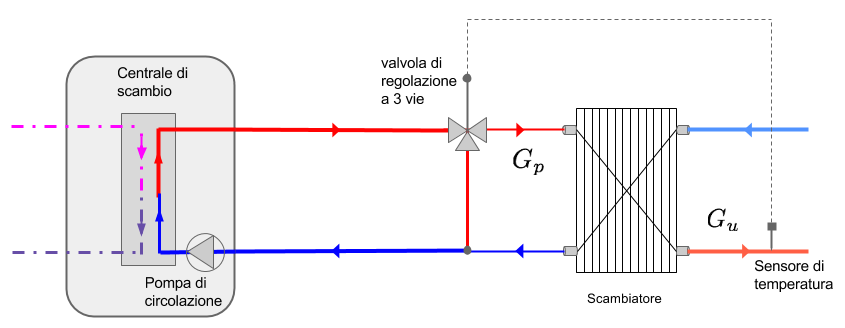
\includegraphics[width=\textwidth]{figure/3vie}
\caption{Schema di funzionamento di una rete con valvola a tre vie.}
\label{fig:3vie}

\end{figure}

Si stabilisce una temperatura di mandata ai radiatori (lato utenza) che dovrà essere mantenuta costante variando la portata in ingresso allo scambiatore. Quando l'abitazione ha bisogno di più energia, la temperatura sul ritorno del lato utenza inizia a diminuire a causa del consumo di calore. Di conseguenza anche il sensore sulla mandata rileva una temperatura più bassa sul circuito d'utenza  e perciò comunica alla valvola a tre vie di aumentare il flusso verso lo scambiatore in modo da avere un più alto trasferimento di calore dalla rete di distribuzione per permettere all'acqua di scaldarsi fino alla temperatura desiderata.
%Quando questa ha bisogno di più energia, la temperatura sul ritorno inizia a diminuire a causa del consumo di calore. La valvola a due vie sul primario  rileva una temperatura più bassa sulla rete di distribuzione e di conseguenza aumenta il flusso in modo da avere un più alto trasferimento di calore dal primario alla rete di distribuzione.
Nel sistema descritto, la valvola a tre vie decide in ogni momento quale è la portata necessaria in base al carico termico richiesto. Il resto dell'acqua è rimandato nella tubazione di ritorno attraverso il by-pass senza essere raffreddata. Conseguentemente, la temperatura di ritorno sarà più alta tanto più acqua è deviata. Più alta è la temperatura sul ritorno dell'utenza     più flusso di acqua sarà necessario per spedire la stessa potenza. In questo sistema la pompa sulla rete di distribuzione lavora sempre a massimo carico, senza dipendere dalla domanda di calore. Conseguentemente la vita delle pompe sarà più breve e le spese di pompaggio saranno alte.

\subsection{Regolazione con valvola di laminazione}
\label{subsec:2vie}
In questo caso, il flusso di acqua non è costante. Una valvola di laminazione (a due vie) regola la portata in base alla necessità di calore delle utenze. 
Come nel caso precedente, quando il sensore rileva una temperatura troppo bassa dell'acqua di mandata del lato utenza, comunica alla valvola di laminazione di far passare più acqua. 
La suddetta valvola può essere vista come una resistenza che si oppone al passaggio del fluido. Maggiore è il grado di laminazione, maggiore è la resistenza offerta e minore risulta la portata della rete di distribuzione. Considerando la pompa a regime costante, il grado di chiusura della valvola fa spostare il suo punto di lavoro lungo la curva caratteristica della pompa stessa, modificando così portata e pressione del fluido.
La portata in ingresso allo scambiatore dipenderà sempre da quanta potenza richiede l'abitazione e questo garantisce una temperatura di ritorno bassa. 
Il consumo di energia dipende in un certo senso dalla quantità di energia termica inviata. Essendo tale potenza variabile sarà possibile risparmiare più energia di pompaggio rispetto al primo caso con la valvola a tre vie dove la potenza inviata è costante. Lo schema di funzionamento è mostrato in Figura \ref{fig:2vie}.

% Figura
\begin{figure}[!ht]
\centering
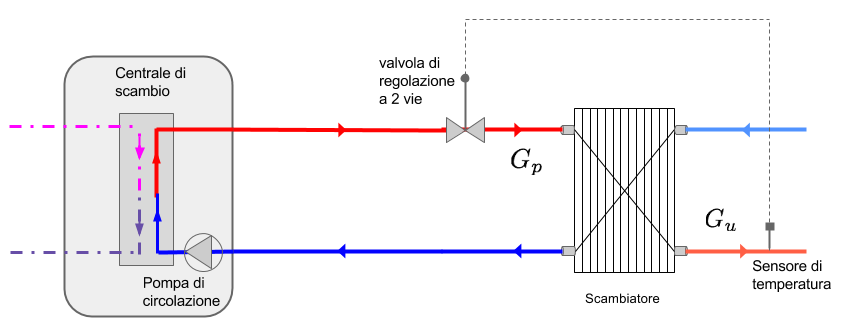
\includegraphics[width=\textwidth]{figure/2vie}
\caption{Schema di funzionamento di una rete con valvola di laminazione (valvola a due vie).}
\label{fig:2vie}

\end{figure}

La rete di distribuzione diventa un sistema con portata e pressione variabile. Viene solitamente scelto dagli ingegneri in quanto ha bisogno di poca manutenzione, riduce i consumi di energia elettrica per il pompaggio e assicura una bassa temperatura di ritorno.

Sia nel primo che nel secondo caso il sensore di temperatura può essere messo sulla tubazione che porta l'acqua ai radiatori anziché su quella di ritorno. In questo modo si definisce un target di temperatura da mantenere. Questo set point dovrà essere impostato in base al tipo di impianto.

\subsection{Regolazione con pompe a temperatura di ritorno costante}
Vengono utilizzate delle valvole a tre vie per regolare il flusso agli scambiatori di utenza. In questo caso però, vi è la possibilità di far variare la velocità delle pompe al fine di ridurre il più possibile i consumi per il pompaggio di acqua.
La velocità viene regolata in modo da mantenere la temperatura dell'acqua di ritorno in centrale di scambio a un valore costante. La temperatura, misurata da un sensore, viene confrontata con quella desiderata e viene valutato se modificare il numero di giri delle pompe. 
Quando un'utenza richiede poca energia termica, la valvola devia gran parte del fluido caldo sulla condotta di ritorno, comportando un aumento della temperatura del liquido. Il sensore rileva questa variazione e comunica alla pompa di diminuire la velocità in quanto l'acqua di ritorno dalle utenze è troppo calda. Ciò implica che il fabbisogno di calore in quel momento è basso e quindi, stiamo inviando più energia di quanta realmente è necessaria. Se l'acqua di ritorno è più fredda del valore desiderato si aumenterà il numero di giri delle pompe. 

Modificando la velocità delle pompe si modifica sia la portata che la prevalenza della stessa (infatti si modifica la sua curva caratteristica) e dunque anche i consumi di energia elettrica. 

\subsection{Regolazione con pompe a pressione differenziale}
Ugualmente alla regolazione descritta nel paragrafo \ref{subsec:2vie}, si utilizza una valvola di laminazione per regolare il flusso di fluido all'utenza ma la principale differenza sta nell'introduzione di una pompa a velocità variabile, controllata in funzione della differenza di pressione tra la condotta di mandata e di ritorno dell'acqua, cosicché il consumo di elettricità per il pompaggio venga ridotto al minimo.
 La velocità della pompa è regolata al fine di mantenere una differenza di pressione costante prestabilita. Le variazioni di pressione nel circuito sono causate dal grado di chiusura della valvola a due vie. Quando la valvola si chiude, aumenta la pressione nel circuito e dei sensori percepiscono la variazione di pressione comunicando alle pompe di modificare il numero di giri in modo da riportare la pressione al valore desiderato. In Figura \ref{fig:giri_variabili} sono analizzati i cambiamenti portati dai due miglioramenti.

% figure
\begin{figure}[!ht]
\centering
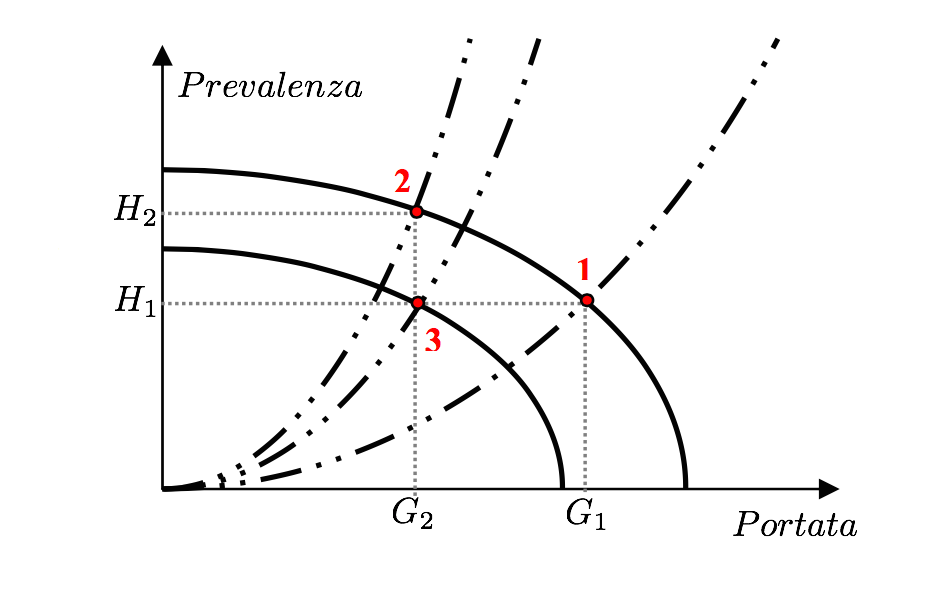
\includegraphics[width=0.8\textwidth]{figure/giri_variabili}
\caption{Curve caratteristiche della pompa (linea continua) e curve caratteristica della rete che descrive la resistenza opposta dalla rete stessa al passaggio dell'acqua (linea tratteggiata).}
\label{fig:giri_variabili}
\end{figure}

Il punto 1 rappresenta un'alta domanda di calore, quindi la portata sarà a sua volta alta. Se la domanda di calore decresce, la valvola di laminazione inizia a chiudersi facendo aumentare la resistenza del circuito e quindi la curva caratteristica della rete, ovvero la curva che descrive la resistenza che oppone la rete al passaggio di una certa portata di acqua, cresce più rapidamente. Il punto di lavoro si sposta quindi da 1 a 2. Il comportamento analizzato fino a ora descrive il funzionamento della valvola di laminazione utilizzato anche nella regolazione a due vie del paragrafo \ref{subsec:2vie}. Se però viene introdotta una pompa a pressione differenziale costante, il punto di funzionamento da 1 verrà spostato a 3. Se la velocità della pompa è diminuita, la caratteristica della pompa verrà descritta da una nuova curva. Anche la curva di carico dell'impianto cambierà, avendo come risultato due curve che si intersecano nel punto 3.      

La regolazione della velocità delle pompe è uno dei modi migliori per diminuire al massimo i consumi delle pompe ed è anche una delle migliori soluzioni per i gestori dell'impianto e per i consumatori. Con questo tipo di regolazione si dovrebbe ottenere il minore consumo di energia e la più alta differenza di temperatura possibile.

%\section{Metodi per ridurre la temperatura di ritorno}  
%% spostare la sezione in un altro capitolo
%
%In una comune utenza la potenza termica necessaria al riscaldamento per raggiungere un certo set point dipende principalmente dalla temperatura esterna. Più all'esterno è freddo più saranno le perdite di calore dell'abitazione.
%
%% ecc..
%


\chapter{Modelli Matematici}

\section{Scambiatore di calore}
\label{subsec:scambiatore_di_calore}
Gli scambiatori di calore sono  delle apparecchiature in cui si realizza lo scambio di energia termica tra due fluidi aventi temperature diverse. Negli impianti di teleriscaldamento solitamente vengono utilizzati scambiatori di calore a piastre, in cui due fluidi scorrono tra delle lastre metalliche piane, dotate di particolari rilievi per aumentare la superficie di scambio termico. In essi la trasmissione del calore avviene per convezione tra i fluidi e le rispettive superfici solide lambite,  e per conduzione attraverso la parete del tubo che li separa. Il tipo di contatto è di tipo indiretto in quanto non vi è miscelazione dei fluidi.
Il loro funzionamento è garantito soltanto dalla presenza di due fluidi a differente temperatura. La temperatura del corpo più caldo diminuisce, mentre la temperatura di quello più freddo aumenta. La progressiva riduzione della differenza di temperatura deve essere ricondotta a uno scambio di energia, scambio che continua finché esiste tale differenza termica, ovvero fino a quando non si raggiunge l'equilibrio termico. 

Le variabili in gioco sono elencate in seguito:
\begin{itemize}
\item[] $G_p$ = portata del circuito primario
\item[]$G_u$ = portata del circuito secondario (parte utenza)
\item[]$c_s$ = calore specifico dell'acqua
\item[]$T_i$ = Temperatura di ingresso scambiatore dalla parte del circuito primario (acqua calda)
\item[]$T_u$ = Temperatura in uscita dallo scambiatore dalla parte del circuito primario (acqua fredda)
\item[]$t_i$ = Temperatura di ingresso scambiatore dalla parte del circuito secondario (acqua fredda)
\item[]$t_u$ = Temperatura in uscita dallo scambiatore dalla parte del circuito secondario (acqua calda)
\end{itemize}

% CAMBIARE IMMAGINE
\begin{figure}[h]
\begin{center}
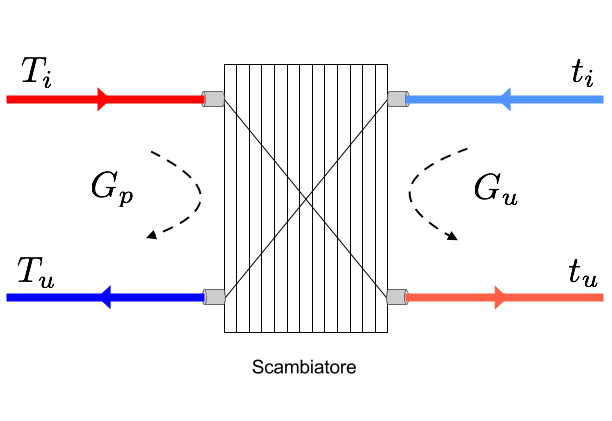
\includegraphics[width=0.65\textwidth]{figure/scambiatore} % Include the image placeholder.png
\caption{Schema di uno scambiatore d'utenza}
\label{fig:scamb}
\end{center}
\end{figure}

Applicando le equazioni di bilancio di massa e di energia al fluido caldo ed al fluido freddo, assumendo che non vi siano dispersioni di calore durante lo scambio, si ottengono le seguenti formule per il calcolo della potenza termica globale $\dot{Q}$. Nello studio degli scambiatori di calore è  utile riferirsi alla cosiddetta portata termica (oraria), $C$, data dal prodotto tra la portata massica ed il calore specifico:
\begin{equation}
C_p=G_p c_s  \ \ \ ; \ \ \ C_u=G_u c_s
\end{equation}
In tal caso le due equazioni di bilancio  possono scriversi nella seguente forma:
\begin{equation}
\dot{Q}=C_p(T_i - T_u) \ \ \ ; \ \ \ \dot{Q}=C_u(t_u - t_i)
\label{eq:scambiatore1}
\end{equation}
A queste due equazioni di bilancio energetico, si può associare una equazione di scambio termico; quest'ultima associa la potenza termica scambiata tra i due fluidi alle temperature di ingresso e/o di uscita, alle portate, al coefficiente di scambio termico globale e all'area di scambio. Questa equazione deriva dal metodo della media logaritmica delle differenze di temperatura (o MLDT) dove  la potenza termica scambiata tra i due fluidi viene legata alla differenza di temperatura tra il fluido caldo ed il fluido freddo dalla seguente relazione:
\begin{equation}
\dot{Q}=\alpha S \Delta T_{ml} ,
\end{equation}
dove
\begin{equation}
 \Delta T_{ml} = \frac{(\Delta T_1)-(\Delta T_2)}{log\left( \frac{\Delta T_1}{\Delta T_2} \right)}.
 \label{eq:scambiatore2}
 \end{equation}
 \begin{center}
 Se scambiatore in corrente : $ \Delta T_1 = T_i - t_i $  \ \ ; \ \ $ \Delta T_2 = T_u - t_u $  \\
 
 Se scambiatore in controcorrente : $ \Delta T_1 = T_i - t_u $  \ \ ; \ \ $ \Delta T_2 = T_u - t_i $ 
\end{center}
dove $S$ \`e  la superficie attraverso cui avviene lo scambio ed $\alpha$ \`e  il cosiddetto coefficiente di scambio termico globale o conduttanza termica unitaria. 

In Figura \ref{fig:andamento} è  possibile vedere l'andamento delle temperature negli scambiatori in corrente (a) e in controcorrente (b).
Nel caso dello scambiatore equicorrente si ha una forte differenza di temperatura all'ingresso e una differenza  minima  all'uscita.  Nel  caso  dello  scambiatore in controcorrente  la  differenza  è invece più costante e il fluido freddo può uscire dallo scambiatore a temperatura maggiore di  quella  dell'uscita del fluido  caldo. 
Termodinamicamente quindi  questa  configurazione  è migliore. 

\begin{figure}[h]
\begin{center}
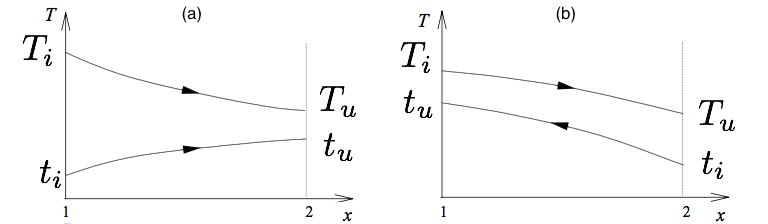
\includegraphics[width=0.95\textwidth]{figure/grafico_scambiatore} % Include the image placeholder.png
\caption{Andamento delle temperature negli scambiatori: (sinistra) caso equicorrente, (destra) caso controcorrente.}
\label{fig:andamento}
\end{center}
\end{figure}

\section{Radiatori}
\label{subsec:radiatori}
I radiatori sono gli elementi all'interno dell'utenza che trasferiscono calore all'ambiente per scaldarlo. 
La potenza emessa da un corpo scaldante dipende dalla temperatura media tra il fluido caldo in ingresso al radiatore e quello freddo in uscita ($t_u$ e $t_i$ rispettivamente) attraverso la seguente relazione:
\begin{equation}
\dot{Q}_{ri}= K_m(\frac{t_u + t_i}{2} - \Theta_{i})^n .
\label{eq:potenza_radiatori}
\end{equation}
I coefficienti $K_m$ e $n$ sono costanti e dipendono dal tipo di radiatore utilizzato. $\Theta_i$ è la temperatura ambiente della casa. 
Il funzionamento di questi elementi di riscaldamento è garantito da una pompa di circolazione solitamente a velocità fissa che permette la circolazione di acqua calda all'interno dell'abitazione. 

Un'analisi importante riguarda il comportamento dei radiatori in termini di calore scambiato al variare della portata. Considerando la temperatura $t_u$ in mandata ai radiatori costante, la temperatura di ritorno dipende  dalla velocità con cui scorre il fluido nei radiatori, quindi la portata è uno dei fattori determinanti della temperatura media e quindi della potenza emessa dai radiatori. Maggiore è la portata minore sarà il tempo per scambiare calore, avendo così una temperatura di ritorno e una conseguente temperatura media più alta e viceversa. Si può fare riferimento all'equazione (\ref{eq:Potenza}), valida anche per i radiatori, per notare come la portata sia direttamente proporzionale alla potenza termica scambiata. 

E' possibile ottenere  le stesse potenze termiche con due portate diverse facendo variare la differenza di temperatura tra fluido caldo e freddo, e di conseguenza alzando o abbassando le temperature di mandata dei radiatori (Figura \ref{fig:portata}). 
%Diminuendo la portata il radiatore scambia di più  e ciò  comporta una riduzione dell'acqua di ritorno dal radiatore. Se però  la temperatura in mandata rimane la stessa avremo una potenza scambiata dal radiatore minore in quanto si \`e  abbassata la temperatura media del fluido all'interno del radiatore (Figura \ref{fig:portata}).

\begin{figure}[h]
\begin{center}
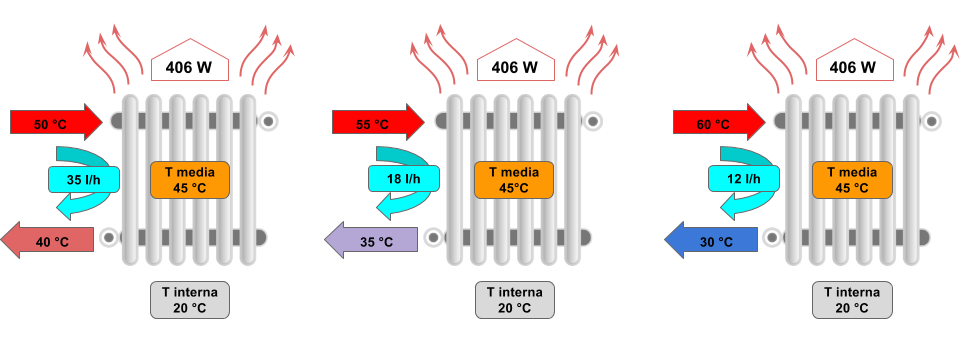
\includegraphics[width=0.95\textwidth]{figure/portata} % Include the image placeholder.png
\caption{Mantenimento delle potenze scambiate dal radiatore a un valore costante variando la temperatura di mandata e la portata.}
\label{fig:portata}
\end{center}
\end{figure}

Dal momento che, come detto in precedenza, le pompe solitamente lavorano a velocità costante, se vogliamo ottenere una potenza maggiore l'unica opzione possibile è quella di aumentare la temperatura in mandata in modo da far aumentare la temperatura media (Figura \ref{fig:portata2}).

\begin{figure}[!ht]
\begin{center}
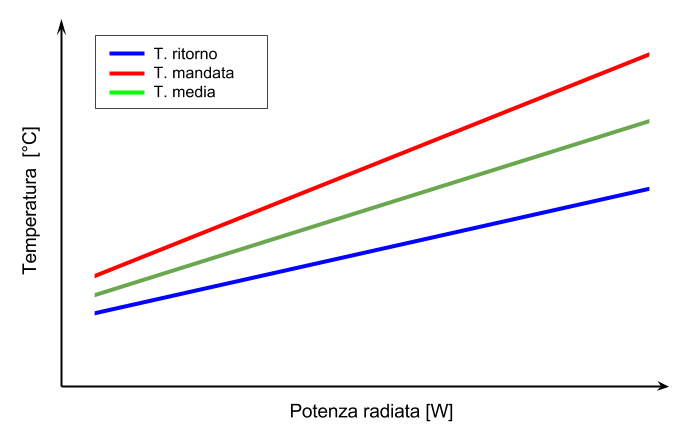
\includegraphics[width=0.85\textwidth]{figure/pot_radiatore} % Include the image placeholder.png
\caption{Variazione delle potenze scambiate dal radiatore variando la temperatura di mandata e mantenendo la portata costante.}
\label{fig:portata2}
\end{center}
\end{figure}

\section{Dinamica dell'utenza}
\label{sec:dinamicautenza}
In seguito è descritto il modello utilizzato in simulazione per modellizzare gli scambi termici all'interno di un edificio. 
Il trasferimento di calore tra due mezzi può avvenire per conduzione o convezione ed è proporzionale alla differenza di temperatura tra i due mezzi coinvolti. Il trasferimento di calore per conduzione e convezione può quindi essere modellizzato utilizzando una resistenza termica,
\begin{equation}
\dot{Q} = \frac{1}{R} (T_1-T_2)
\label{eq:q1}
\end{equation}
dove $T_1$ e $T_2$ sono le temperature di ogni mezzo coinvolto nello scambio di calore mentre $R$ è la resistenza opposta al trasferimento l'energia termica.

L'altro aspetto importante da tenere in considerazione è la capacità termica, la quale descrive quanto un materiale  è in grado di accumulare calore. Nella seguente equazione è descritta la relazione che lega la capacità termica $C$ con il calore trasferito $\dot{Q}$ e la temperatura $T$.
\begin{equation}
\dot{Q} = C(T) \frac{dT}{dt} \approx C \frac{dT}{dt}
\label{eq:q2}
\end{equation}
Dal momento che l'intervallo di temperature in cui opera la casa è piccolo, possiamo  assumere la capacità termica come costante.

La termodinamica dell'utenza è modellata come una grande stanza circondata da pareti. I relativi flussi termici sono schematizzati in Figura \ref{fig:scambio}. Gli scambi di calore che possono avvenire sono: scambio di calore tra i radiatori e l'aria della stanza, scambio di calore tra l'aria della stanza e le pareti, scambio di calore tra le pareti e l'esterno.

\begin{figure}[h]
\begin{center}
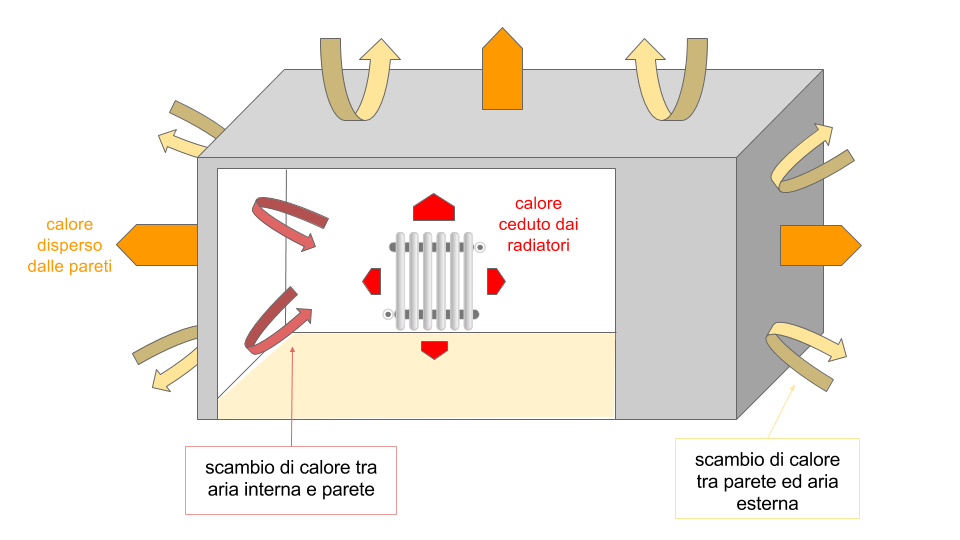
\includegraphics[width=1.05\textwidth]{figure/scambio_casa}
\caption{Scambi di calore di un'abitazione generica.}
\label{fig:scambio}
\end{center}
\end{figure}

Le grandezze che verranno usate nel modello da questo punto in avanti sono le seguenti:
\begin{itemize}
\item[] $\dot{Q}_{ri}$ = calore fornito dai radiatori
\item[]$C_a$ = Capacità termica dell'aria 
\item[]$C_p$ = Capacità termica delle pareti
\item[]$c_a$ = Calore specifico dell'aria 
\item[]$c_p$ = Calore specifico delle pareti
\item[]$c_s$ = Calore specifico dell'acqua
\item[]$R_{ip}$ = Resistenza termica tra l'aria interna alla casa e la parete 
\item[]$R_{pe}$ = Resistenza termica tra la parete e l'aria all'esterno della casa
\item[]$R_{f}$ = Resistenza termica offerta dalle finestre 
\item[]$R_{conv,i}$ = Resistenza termica per convezione della  parete interna della casa
\item[]$R_{conv,e}$ = Resistenza termica per convezione della  parete esterna della casa
\item[]$R_{cond}$ = Resistenza termica per conduzione della parete della casa
\item[]$\Theta_{e}$ = Temperatura dell'aria all'esterno della casa
\item[]$\Theta_i$ = Temperatura dell'aria all'interno dalla casa
\item[]$\Theta_p$ = Temperatura della superficie della parete all'interno dalla casa 
%\item[]$A$ = Superficie di scambio delle pareti
\end{itemize}


A causa delle analogie tra le equazioni (\ref{eq:q1}) e (\ref{eq:q2}) con resistenze e capacità elettriche, possiamo modellizzare la termodinamica dell'abitazione come una rete elettrica, costituita da resistenze e condensatori, con le temperature equivalenti alle tensioni e il flusso di calore equivalente al flusso di cariche elettriche, ovvero alla corrente. Il circuito elettrico equivalente degli scambi di calore è mostrato in Figura \ref{fig:RC}.

\begin{figure}[h]
\begin{center}
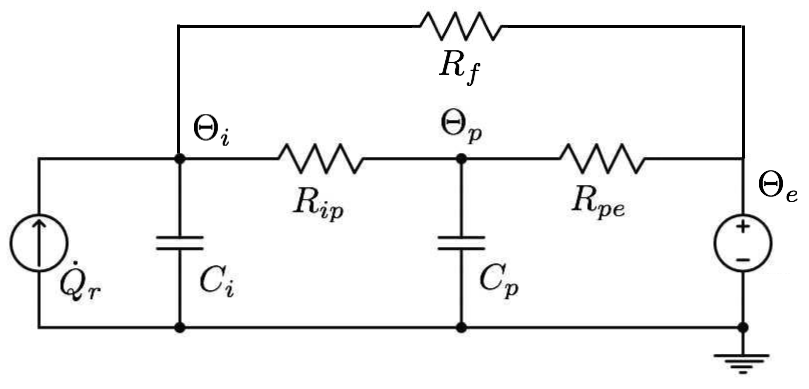
\includegraphics[width=0.75\textwidth]{figure/schema_trasf_calore}
\caption{Circuito equivalente RC per gli scambi di calore.}
\label{fig:RC}
\end{center}
\end{figure}
 
Vediamo adesso in dettaglio come viene considerato lo scambio tra aria pareti ed esterno. L'aria interna che precedentemente ha ricevuto calore dai radiatori cede calore alla superficie interna delle pareti per convezione secondo la legge:
\begin{equation}
\dot{Q} = \frac{(\Theta_i - \Theta_p)}{R_{ip}} ,
\end{equation} 
e cede calore direttamente all'esterno per mezzo delle finestre secondo la legge in seguito:
\begin{equation}
\dot{Q} = \frac{(\Theta_i - \Theta_e)}{R_{f}} .
\end{equation} 
Dal momento che la temperatura delle pareti a cui facciamo riferimento è quella della superficie interna dell'edificio, la resistenza termica sarà data soltanto dalla resistenza termica per convezione, ovvero:
\begin{center}
$R_{ip} = R_{conv,i}$
\end{center}

Lo scambio tra la parete e l'ambiente esterno è dato dalla differenza di temperatura tra la parete interna e l'aria  esterna, considerando come resistenza termica la resistenza conduttiva $R_{cond}$ degli strati della parete e la resistenza convettiva sulla superficie esterna $R_{conv,e}$ per cui:
\begin{equation}
\dot{Q} = \frac{(\Theta_p - \Theta_e)}{R_{pe}} 
%R_{conv,e} = \frac{1}{h_{conv,e}}
\end{equation} 
\begin{center}
$R_{pe} = R_{cond} + R_{conv_e}$
\end{center}

Il modello può essere formulato come un modello a parametri concentrati a due stati di temperatura: la temperatura dell'aria all'interno della casa $\Theta_i$ e la temperatura delle pareti $\Theta_p$.

Riassumendo, l'aria, riscaldata dai radiatori a temperatura $\Theta_i$, scambia calore con la superficie interna delle pareti che si troverà a temperatura $\Theta_p$. In base alla superficie di scambio, la differenza di temperatura tra i due mezzi e la resistenza termica $R_{ip}$ tra aria e pareti, si otterrà un certo scambio termico verso di esse. L'energia scambiata viene accumulata dalla parete che funziona come un condensatore di capacità $C_p$. Parte dell'energia totale delle pareti invece viene ceduta all'esterno. Il calore ceduto dipenderà dalla superficie di scambio, dalla differenza di temperatura tra la parete interna e l'aria all'esterno dell'edificio, e la resistenza termica $R_{pe}$ che offre la parete con l'aria esterna. Un'altra parte di energia è scambiata dall'aria verso l'esterno attraverso le finestre.  

Un equivalente elettrico del modello della parete è visibile in Figura \ref{fig:RC_parete}.
Quando la potenza scambiata dall'aria con la parete  interna è maggiore di quella dispersa all'esterno si avrà un aumento della temperatura delle pareti stesse.

Da notare è anche il fatto che la temperatura all'interno della parete non è uniforme. Infatti, se prendessimo una sezione di una parete, vedremmo che in base alla distanza dalla sua superficie interna la temperatura decresce come mostrato in Figura \ref{fig:temp_parete}.  Nel modello scelto si considera come temperatura di riferimento della parete la temperature della superficie interna della stessa. La scelta è stata fatta solamente per comodità, infatti si sarebbe potuto tenere in considerazione la temperatura della superficie esterna anziché quella interna. In base al punto al quale si fa riferimento per la temperatura, sarà necessario impostare  i valori di $R_{ip}$ e $R_{pe}$ appropriatamente.   

 \begin{figure}[!ht]
 \centering
 \subfigure[Circuito equivalente RC di una parete.\label{fig:RC_parete}]
   {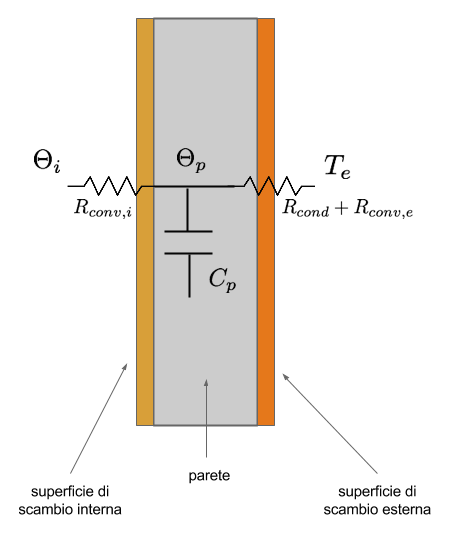
\includegraphics[width=9cm]{figure/RC_parete}}
 \hspace{5mm}
 \subfigure[Andamento della temperatura in una parete.\label{fig:temp_parete}]
   {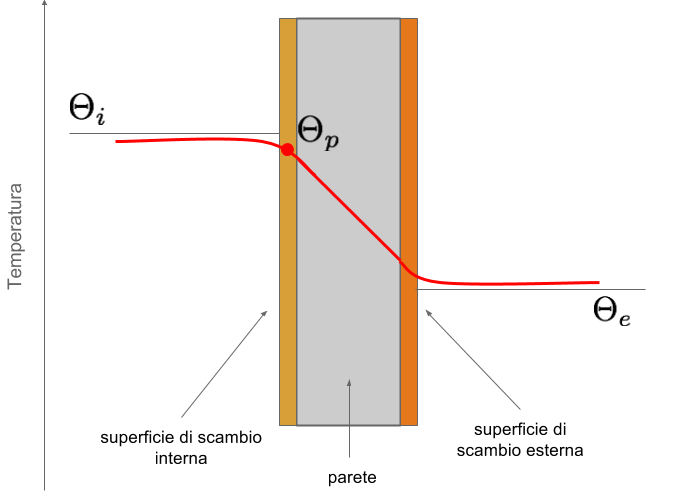
\includegraphics[width=9cm]{figure/temp_parete}}
 \caption{Schemi di funzionamento degli scambi termici in una parete di un'abitazione.}
 \end{figure}



\section{Dinamica e interazioni tra scambiatore e utenza}
Per quanto riguarda la creazione di un simulatore dobbiamo trovare un modello matematico che descriva le interazioni che avvengono tra lo scambiatore di calore e l'utenza. In particolare è interessante sapere come si evolvono le temperature dell'acqua nello scambiatore e come varia la temperatura interna dell'abitazione al variare di alcuni parametri come la temperatura in ingresso allo scambiatore, la temperatura in mandata verso i radiatori, la portata, sia del lato della rete di distribuzione che del circuito dell'utenza, e la temperatura esterna.
In Figura \ref{fig:scamb_utenza} è rappresentato lo schema che descrive le interazioni e i parametri in gioco nel sistema composto dallo scambiatore di calore e dall'utenza. 

\begin{figure}[h]
\begin{center}
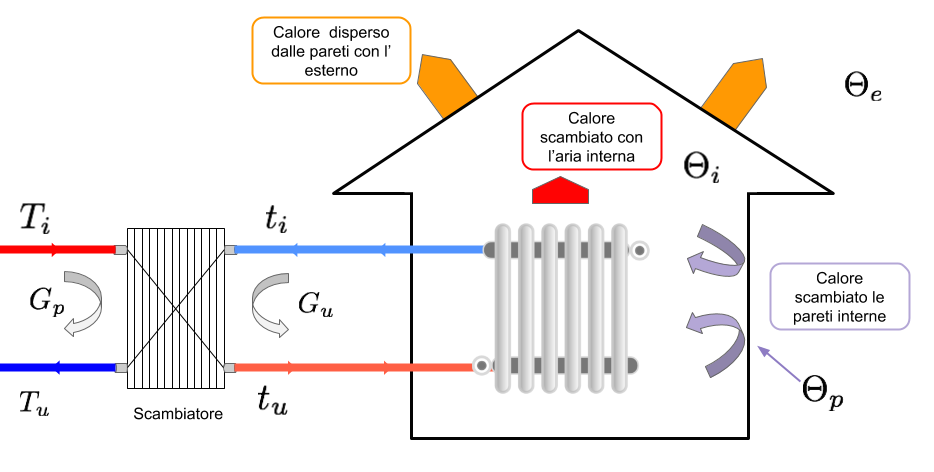
\includegraphics[width=\textwidth]{figure/scamb_utenza} % Include the image placeholder.png
\caption{Rappresentazione schematica sistema scambiatore e utenza}
\label{fig:scamb_utenza}
\end{center}
\end{figure}

%Come descritto nella sezione \ref{sec:dinamicautenza} 
Faremo riferimento a un sistema dinamico con due variabili di stato: la temperatura interna all'utenza  $\Theta_i$  e  temperatura della superficie interna delle pareti  $\Theta_p$. Il sistema è  descritto  da due equazioni differenziali:
\begin{center}
$M_ac_a \dot{\Theta}_i = \dot{Q}_{ri} - \dot{Q}_{ip} - \dot{Q}_{if}$ 
\end{center}
\begin{center}
$M_pc_p \dot{\Theta}_p = \dot{Q}_{ip} - \dot{Q}_{pe}$
\end{center}
con $\dot{Q}_{ri}$ il\ calore scambiato tra i radiatori e l'aria interna alla casa, $\dot{Q}_{ip}$ il calore scambiato tra l'aria e la parete interna,$\dot{Q}_{if}$ il calore scambiato tra l'aria e l'esterno attraverso le finestre, $M_a$ la massa dell'aria all'interno dell'abitazione e $c_a$ è il calore specifico dell'aria. Per la seconda equazione $ \dot{Q}_{pe}$ è il calore scambiato tra le pareti e l'ambiente esterno, $M_p$ la massa delle pareti e $c_p$ il calore specifico delle pareti.
Più in particolare:
\begin{equation}
K_m\left(\frac{t_u + t_i}{2} - \Theta_{i}\right)^n - \left(\frac{\Theta_{i} - \Theta_p}{R_{ip}}\right) - \left(\frac{\Theta_{i} - \Theta_e}{R_{f}}\right) = M_ac_a \dot{\Theta_i}
\end{equation}
\begin{equation}
\left(\frac{\Theta_{i} - \Theta_p}{R_{ip}}\right) - \left(\frac{\Theta_{p} - \Theta_e}{R_{pe}}\right) = M_pc_p \dot{\Theta_p}
\end{equation}



\`E possibile analizzare due differenti scenari:
\begin{itemize}
\item \textbf{Scambiatore senza regolazione di portata}: si tratta di avere uno scambiatore d'utenza senza alcun tipo di regolazione sulla portata. In questo caso non è possibile definire nessun set point di temperatura in mandata ai radiatori. Le variabili note sono $G_u, T_i, G_p$ mentre quelle incognite sono: $T_u, t_u, t_i$

\item \textbf{Scambiatore con regolazione di portata}: si analizza uno scambiatore con regolazione sulla portata. Con questo tipo di configurazione vi è la possibilità di fissare la temperatura in mandata ai radiatori. Questa temperatura viene mantenuta costante agendo su una valvola di laminazione che regola la portata in arrivo allo scambiatore dal lato della rete di distribuzione.   Le  variabili note sono $G_u, T_i, t_u$ mentre quelle incognite sono: $G_p, T_u, t_i$
\end{itemize}
Assumendo che la potenza termica scambiata dallo scambiatore sia uguale alla potenza emessa dai radiatori, le incognite degli scenari sopra citati, si possono ricavare dal seguente sistema di  tre equazioni in tre incognite: 
\begin{equation}
\left \{
\begin{array}{rl}
K_m(\dfrac{t_u + t_i}{2} - \Theta_{amb})^n = G_u c_s (t_u - t_i)\\
\\
G_p c_s (T_i - T_u) = G_u c_s (t_u - t_i)\\
\\
G_u c_s (t_u - t_i) = \alpha S \dfrac{(T_i - t_u)-(T_u - t_i )}{log\left( \dfrac{T_i - t_u}{T_u - t_i } \right)}\\
\end{array}
\right.
\end{equation}

Le equazioni mettono in relazione la potenza emessa dai radiatori descritta nell' equazione (\ref{eq:potenza_radiatori}) con il bilancio termico e la potenza scambiata dallo scambiatore descritta nelle equazioni (\ref{eq:scambiatore1}) e (\ref{eq:scambiatore2}) rispettivamente.

\section{Dinamica della rete di distribuzione}
Qualsiasi rete di tubature attraversata da fluidi in pressione è affetta da perdite di carico ovvero da perdite di pressione dovute all'insieme delle forze passive (scabrezza dei materiali, dislivelli, curve e derivazioni) che oppongono una resistenza allo scorrimento dell'acqua. L'espressione più generale che lega la perdita di carico $J$ per unità di lunghezza della condotta di un fluido incomprimibile in moto stazionario è quella di Darcy-Weisbach \cite{darcy}:
\begin{equation}
J = \frac{\lambda \ v^2}{2 \ g \ D}
\end{equation}
avendo indicato con $D$ il diametro della condotta, $v$ la velocità del fluido, $g$ l'accelerazione di gravità e $\lambda$ un coefficiente adimensionale di resistenza, che è funzione, in generale, della scabrezza relativa del tubo e del numero di Reynolds:
\begin{equation}
R_e = \frac{\rho \ v \ D}{\mu}
\end{equation}
con $\rho$ e $\mu$ la densità e la viscosità dinamica del fluido, rispettivamente. 
Per trovare la perdita di carico in una condotta dal punto $i$ al punto $j$ di lunghezza $L$ non si dovrà altro che moltiplicare la perdita di carico per unità di lunghezza $J$ per la lunghezza del tubo:
\begin{equation}
\Delta P_{ij} = J \ L
\end{equation} 
 
Più in particolare in Figura \ref{fig:perdite_carico} è illustrato uno schema di una piccola parte della rete di distribuzione dell'impianto.

\begin{figure}[h]
\centering
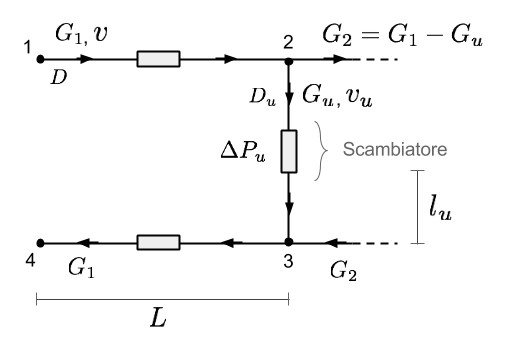
\includegraphics[width=0.70\textwidth]{figure/perdite_carico} % Include the image placeholder.png
\caption{Schema rappresentativo delle perdite di carico di una porzione della rete di distribuzione.}
\label{fig:perdite_carico}

\end{figure}

Dal punto 1 al punto 2 vi è la condotta della rete principale con diametro $D$ che trasporta l'acqua calda mentre da 3 a 4 è la condotta, sempre della rete principale con diametro uguale a quello della condotta da 1 a 2 che trasporta l'acqua raffreddata in ritorno alla centrale di scambio. Entrambe le  condotte sono di lunghezza $L$ identica, in quanto negli impianti le condotte sono sempre poste l'una affianco dell'altra. L'acqua scorre a velocità $v$.

Il punto 2 è il punto in cui avviene il prelievo dalla rete principale per portare l'acqua calda all'utenza. Da 2 a 3 abbiamo quindi la condotta che porta l'acqua all'utenza e una che dall'utenza riporta l'acqua alla condotta di ritorno dell'acqua raffreddata con velocità $v_u$. La lunghezza totale è $2 \cdot l_u$ ed il diametro è $D_u$.

Ad ogni condotta può essere associata una certa resistenza che  indica quanto questa si oppone al flusso dell'acqua. Da 2 a 3 oltre alle perdita di carico dovute alle tubazioni vi è anche la perdita di carico che offre lo scambiatore di calore:
\begin{equation}
\Delta P_s = K \ G^2_u
\end{equation}
con K costante che dipende dal tipo di scambiatore.

Le equazioni che descrivono le perdite di carico del sistema sono:

\begin{equation}
\begin{cases}
\Delta P_{12} = \dfrac{\lambda v^2}{2 g D} L = \Delta P_{34} \\
\\
\Delta P_{23} = \dfrac{\lambda v_u^2}{ g D_u} l_u + \Delta P_s
\end{cases}
\end{equation}

Le precedenti equazioni sono usate per ricavare le portate in arrivo alle utenze $G_u$, che rappresentano le variabili incognite d'interesse del sistema descritto. Le portate $G_u$ dipendono principalmente dalla differenza di pressione $\Delta P_{23}$: infatti se questa non è sufficientemente grande, non sarà garantito il corretto funzionamento dello scambiatore.

Dal momento che si tratta di un modello fortemente non lineare, si procede all'analisi della rete in modo iterativo. Partendo da dei valori di portata e prevalenza emessi dalla pompa si ricava la portata $G_u$ della prima utenza incontrata e la portata $G_2$ che andrà ad alimentare tutte le utenze restanti. A questo punto si può continuare l'analisi della rete spostando l'attenzione all'utenza successiva, ripetendo le operazioni fatte precedentemente, considerando però come portata della condotta principale $G_1$ la portata $G_2$, e così via fino a quando tutte le utenze sono state analizzate.

Nel caso in cui lo scambiatore d'utenza disponga di una regolazione della portata, allora tale portata, non dipenderà più direttamente dalla differenza di pressione tra i punti 2 e 3, ma sarà determinata dal grado di laminazione della valvola dello scambiatore. 

\section{Perdite di calore nella rete}
Per perdita di calore si intende un trasferimento di 
energia termica tra due sistemi, che è causato da una differenza di temperatura tra i due sistemi in questione. Il calore ceduto da un sistema, a temperatura maggiore, viene acquistato dal secondo sistema, in accordo con la legge di conservazione dell'energia. 
Le perdite di calore in una rete di teleriscaldamento sono proporzionali alla differenza di temperatura tra l'acqua che circola nelle condotte e il terreno. Le tubazioni a cui facciamo riferimento sono composte da tubi in acciaio rivestiti da una schiuma isolante poliuretanica, interrati a qualche decina di centimetri.
Le perdite sono quantificate secondo le indicazioni delle norme B.S. (British Standard), assumendo per il coefficiente di conducibilità della schiuma il valore indicato dalle norme CEN EN253 ed utilizzando la formula:

\begin{equation}
\dot{Q}_{disp} = \dfrac{4 \varphi (T_M - T_S)}{\dfrac{1}{\lambda_{PU}} \cdot ln \left(  \dfrac{D - 2t}{d}\right)  + \dfrac{1}{\lambda_S} \cdot ln \left(  \dfrac{2H_S + D}{D}\right) }
\end{equation}
dove:
\begin{itemize}
\item[] $\varphi = \left[ 180 - arctan  D /( D + A_S)  \right] \cdot \pi/180 $  
\item[] $T_S =$ temperatura del suolo circostante i tubi
\item[] $T_M =$ media delle temperature di mandata e ritorno del fluido
\item[] $H_S =$ Altezza del terreno sopra i tubi
\item[] $A_S =$ spazio tra i tubi in PEAD (polietilene ad alta densità)
\item[] $d =$ diametro esterno del tubo in acciaio
\item[] $D =$ diametro esterno del tubo in PEAD
\item[] $t =$ spessore del tubo in PEAD
\item[] $\dot{Q}_{disp} =$ Perdita di calore totale per mandata e ritorno per unità di lunghezza
\item[] $\lambda_S =$ coefficiente di conduzione termica del suolo
\item[] $\lambda_{PU} =$ coefficiente di conduzione termica del poliuretano
\end{itemize}

\section{Pompe di circolazione}
Nei sistemi di teleriscaldamento considerati nell'elaborato la circolazione dell'acqua nella rete è resa possibile grazie a delle pompe centrifughe. Queste pompe sono essenzialmente costituite da una girante a palette che gira in una camera a forma di chiocciola [Figura \ref{fig:pompa_centrifuga}], comunicante con la tubazione di aspirazione al centro e con la tubazione di mandata alla periferia.

\begin{figure}[h]
\centering
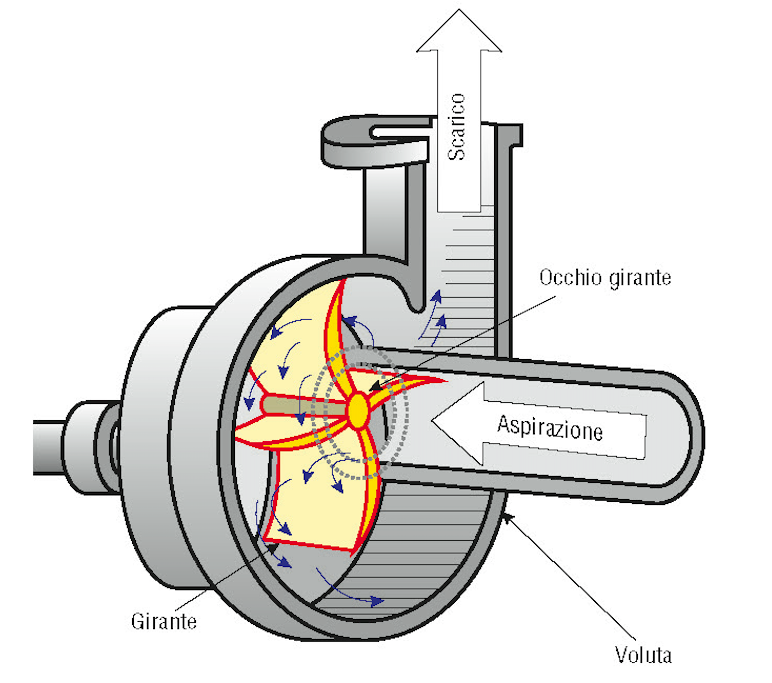
\includegraphics[width=0.65\textwidth]{figure/pompa_centrifuga} 
\caption{Pompa centrifuga con diffusore a palette}
\label{fig:pompa_centrifuga}
\end{figure}

Durante il funzionamento, le palette della girante trascinano in rotazione il liquido e la carcassa lo convoglia verso la tubazione di mandata.
Si determina così una depressione al centro, che richiama altro liquido dalla tubazione di aspirazione, e una spinta in periferia, verso il tubo di mandata.
L'energia acquisita dal liquido attraverso la pompa, cioè la prevalenza manometrica, è in questo caso direttamente proporzionale al quadrato della velocità periferica della girante.
La sezione della camera cresce gradatamente, dall'origine allo sbocco, di pari passo con l'aumentare del liquido che esce uniformemente dalle palette della girante.
La pompa per poter sollevare il fluido deve
essere adescata, cioè sia il condotto di
aspirazione, sia il corpo della pompa devono essere sempre pieni di liquido. Ciò si realizza disponendo all'inizio del condotto di aspirazione una valvola di fondo (o di non ritorno), che permette il passaggio del liquido solo in una direzione e precisamente dal serbatoio alla condotta di aspirazione.
Le pompe centrifughe hanno in genere un rendimento sensibilmente inferiore a quello delle pompe alternative, principalmente per effetto delle maggiori perdite volumetriche. Sono però notevolmente le più diffuse, per la semplicità di funzionamento, di costruzione, e perché possono essere collegate direttamente con i motori elettrici ed endotermici; inoltre non avendo valvole, possono funzionare bene anche con liquidi fangosi.
\subsection{Curve caratteristiche}
La portata e la prevalenza delle pompe centrifughe variano in funzione del numero di giri. Inoltre, con il variare della portata varia anche la prevalenza e viceversa. Riportando, in un sistema di assi cartesiani, in ascissa i valori della portata e in ordinata i corrispondenti valori della prevalenza, si ottiene la curva caratteristica della pompa per il numero di giri considerato [Figura \ref{fig:curve_car}].

\begin{figure}[!ht]
\centering
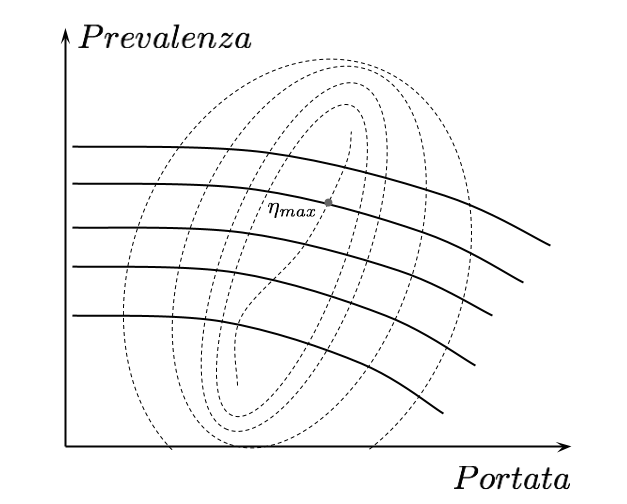
\includegraphics[width=0.65\textwidth]{figure/curve_car} 
\caption{Curve caratteristiche di una pompa centrifuga al variare del numero di giri (linea continua) e curve di rendimento collinari (linea tratteggiata).}
\label{fig:curve_car}
\end{figure}

L'andamento delle curve caratteristiche si può determinare sperimentalmente.
Per questo, sul banco di prova e con la pompa al regime voluto, si varia la portata, agendo
su una valvola di mandata, e per ogni valore della portata si misura il valore della
prevalenza mediante due manometri, uno sulla mandata e uno sull'aspirazione.
Il rendimento della pompa per il regime considerato è massimo solo in un determinato punto della curva.
Congiungendo tutti i punti nei quali il rendimento ha lo stesso valore, si ottengono delle curve chiuse e concentriche, dette curve di uguale rendimento, o di isorendimento; la linea che unisce i punti di massimo rendimento ($\eta_{max}$) risulta però aperta, perché non esistono in una curva due punti di massimo rendimento.

\subsection{Legge di affinità}
Per le pompe centrifughe esiste una legge che mette in relazione portata, prevalenza e potenza con il numero di giri $n$.
La portata $G$ di una pompa centrifuga varia proporzionalmente al numero di giri; la prevalenza $H_m$ varia proporzionalmente al quadrato del numero di giri; la potenza utile $P$, proporzionale al prodotto della portata per la prevalenza, varia proporzionalmente al cubo del numero di giri:
\begin{equation}
\frac{Q_1}{Q_2}=\frac{n_1}{n_2} \quad \qquad  \frac{H_{m1}}{H_{m2}}=\left( \frac{n_1}{n_2}\right)^2 \quad \qquad  \frac{P_1}{P_2}=\left( \frac{n_1}{n_2}\right)^3
\label{eq:affinita}
\end{equation}
Queste tre espressioni esprimono la legge d'affinità, la quale permette di tracciare la curva caratteristica di una pompa a un regime di rotazione $n_2$ quando è nota la curva relativa a un regime di rotazione $n_1$, non molto dissimile da $n_2$.

\begin{figure}[!ht]
\centering
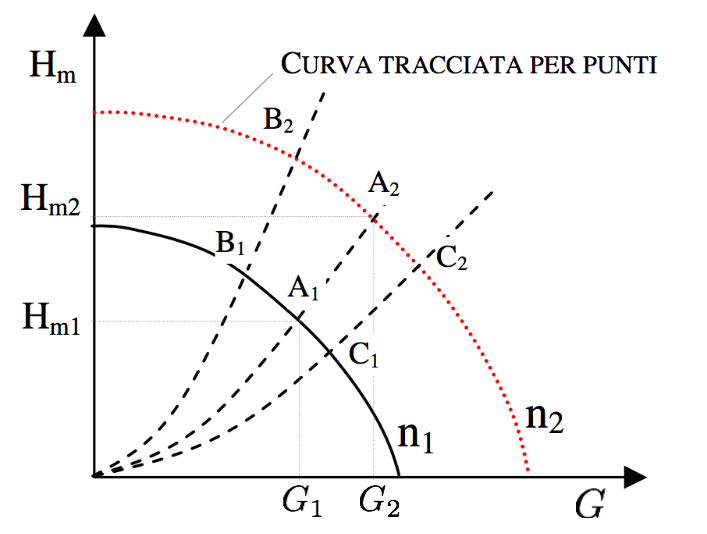
\includegraphics[width=0.65\textwidth]{figure/affinita} 
\caption{Utilizzo della legge di affinità per ricavare da una curva caratteristica nota a regime di rotazione $n_1$ un'altra curva caratteristica avente regime di rotazione $n_2$.}
\label{fig:affinita}
\end{figure}

Facendo riferimento alla Figura \ref{fig:affinita}, noti per il punto $A_1$ i valori di $G_1$ e $H_{m1}$, si possono determinare:

\begin{center}
$G_2 = \dfrac{n_2}{n_1} \ G_1 \qquad e \qquad H_{m2} = \left( \dfrac{n_2}{n_1}\right)^2  H_{m1}$
\end{center}

che individuano il punto $A_2$. Procedendo in modo analogo per i punti $B_1$, $C_1$ si determinano i corrispondenti punti $B_2$, $C_2$.La curva ottenuta unendo tutti questi punti rappresenta la caratteristica della pompa al regime di rotazione $n_2$.

I punti $A_1$ e $A_2$, $B_1$ e $B_2$, $C_1$ e $C_2$, appartengono a una parabola avente il vertice nell'origine degli assi, infatti dalla legge di affinità:
\begin{center}
$\dfrac{H_{m1}}{H_{m2}}=\left(\dfrac{n_1}{n_2} \right)^2 = \left(\dfrac{G_1}{G_2} \right)^2  \qquad$ ovvero   $\qquad \dfrac{H_{m1}}{G_1^2}=\dfrac{H_{m2}}{G_2^2}$ 
\end{center}
In generale quindi $H_m = K \ G^2$ che corrisponde all'equazione di una parabola passante per l'origine che descrive la resistenza che oppone il circuito alimentato dalla pompa.

La legge di affinità implica che il rendimento della pompa resti invariato alle due velocità. Quindi, due punti appartenenti alla stessa parabola che descrive la caratteristica del circuito risultano avere lo stesso rendimento. In realtà, ciò non è completamente corretto.


\subsection{Potenza assorbita da una pompa}
La pompa, per sollevare una portata d'acqua $G$ fornendole una prevalenza totale $H_m$ compie un lavoro di sollevamento che richiede una potenza $P_u$ (misurata in watt), cioè un'energia, fornitale attraverso un motore, definita dalla seguente espressione:
\begin{equation}
P_u = \rho \ g \ Q \ H_m
\end{equation}
con $\rho$ uguale alla densità del fluido e $g$ l'accelerazione di gravità.
La potenza così espressa è la potenza utile, cioè quella strettamente necessaria per sollevare la portata d'acqua $Q$ all'altezza $H_m$. A causa delle inevitabili perdite d'energia la potenza utilizzata, cioè quella realmente necessaria per far funzionare la pompa, è maggiore e viene definita potenza assorbita $P_a$:
\begin{equation}
P_a = \dfrac{\rho \ g \ Q \ H_m}{\eta}
\label{eq:pot}
\end{equation}
Il rapporto fra la potenza utile e quella assorbita è definito rendimento ($\eta$). Il rendimento è sempre inferiore all'unità perché in qualsiasi macchina operatrice la potenza utile è sempre minore di quella assorbita. 

\section{Controllo PID}
Il controllo Proporzionale-Integrale-Derivativo, comunemente abbreviato come PID \cite{visioli2006practical}, è un sistema in retroazione negativa ampiamente impiegato nei sistemi di controllo. È il sistema di controllo in retroazione di gran lunga più comune nell'industria, in particolare nella versione PI (senza azione derivativa). 
La reazione all'errore può essere regolata e ciò rende questo sistema molto versatile.

Il controllore acquisisce in ingresso un valore da un processo, e lo confronta con un valore di riferimento. La differenza, il cosiddetto segnale di errore, viene  usato per determinare il valore della variabile di uscita del controllore, che è la variabile manipolabile del processo, in maniera da tendere verso un errore nullo.\\

Il PID regola l'uscita in base a:
\begin{itemize}
\item il valore del segnale di errore (azione proporzionale);
\item i valori passati del segnale di errore (azione integrale);
\item quanto velocemente il segnale di errore varia (azione derivativa).
\end{itemize}

Le tre azioni di un PID vengono calcolate separatamente e semplicemente sommate algebricamente:
\begin{equation}
u=u_P + u_I + u_D 
\end{equation}

L'azione proporzionale è ottenuta moltiplicando il segnale d'errore $e$ con un'opportuna costante $K_P$:
\begin{equation}
u_P = K_P \ e
\end{equation}

L'azione integrale è proporzionale all'integrale nel tempo del segnale di errore $e$, moltiplicato per la costante $K_I$:
\begin{equation}
u_I = K_I \int e(t) dt
\end{equation}
Questa definizione dell'azione integrale fa sì che il controllore abbia memoria dei valori passati del segnale d'errore; in particolare, il valore dell'azione integrale non è necessariamente nullo se è nullo il segnale d'errore. Questa proprietà dà al PID la capacità di portare il processo esattamente al punto di riferimento richiesto, dove la sola azione proporzionale risulterebbe assente.

Per migliorare le prestazioni del controllore si può aggiungere l'azione derivativa:
\begin{equation}
u_D = K_d \ \dfrac{de}{dt} 
\end{equation}
L'idea è compensare rapidamente le variazioni del segnale di errore: se vediamo che $e$ sta aumentando, l'azione derivativa cerca di compensare questa deviazione in ragione della sua velocità di cambiamento, senza aspettare che l'errore diventi significativo (azione proporzionale) o che persista per un certo tempo (azione integrale).
Il funzionamento è riassunto nello  schema a blocchi in Figura \ref{fig:PID2}.

\begin{figure}[!ht]
\centering
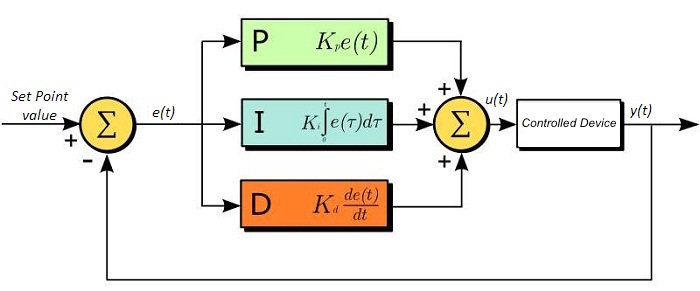
\includegraphics[width=0.95\textwidth]{figure/PID2} 
\caption{Schema a blocchi del funzionamento di un controllore PID.}
\label{fig:PID2}
\end{figure}

Questo particolare controllore verrà in seguito utilizzato per regolare la portata in ingresso ad uno scambiatore agendo su una valvola di laminazione definendo in ogni istante quale dovrà essere la temperatura di mandata ai radiatori desiderata.

\chapter{Risultati di simulazione}
L'ottimizzazione e il controllo delle reti di teleriscaldamento è di grande interesse per industria energetica a causa dei vantaggi tecnici, economici e ambientali che potrebbero essere guadagnati da una gestione adeguata. Tuttavia, i modelli di questi sistemi complessi sono fortemente non lineari  e soffrono di incertezze rilevanti. in questo lavoro di tesi, è stato implementato un simulatore di una rete di teleriscaldamento per analizzare e confrontare diverse strategie di controllo che riducano al minimo i costi di gestione di un impianto.
Il punto di partenza per ottimizzare l'intero impianto consiste nell'incrementare l'efficienza delle utenze, abbattendo al massimo la temperatura dell'acqua di ritorno dagli scambiatori 
e riducendo gli sprechi, anche a fronte di una poco oculata gestione della regolazione della temperatura all'interno delle abitazioni.

La calibrazione del modello di simulazione è stata eseguita confrontando le uscite del modello con dati misurati sul campo.
In particolare, è stato preso in esame un piccolo impianto di teleriscaldamento composto da undici utenze. Nonostante le ridotte dimensioni, il suo studio risulta di particolare interesse in quanto l'impianto, a causa di un cattivo sistema di regolazioni, fa registrare costi di gestione siano quasi sempre vicini al massimo stagionale (consumi che si hanno nel periodo più freddo dell'anno). Inoltre, le ridotte dimensioni  hanno semplificato l'implementazione del modello di simulazione e la raccolta dei dati necessari alla calibrazione del sistema.  

\section{Influenza della temperatura esterna sulla gestione di un sistema di teleriscaldamento}
Le stazioni termiche sono progettate in modo da fornire agli utenti il calore necessario per il riscaldamento delle abitazioni nei periodi più freddi dell'anno.

In Figura \ref{fig:profilo_temp} è mostrato l'andamento della temperatura media esterna riferita all'area geografica del comune di Pomarance (PI).

\begin{figure}[!ht]
\centering
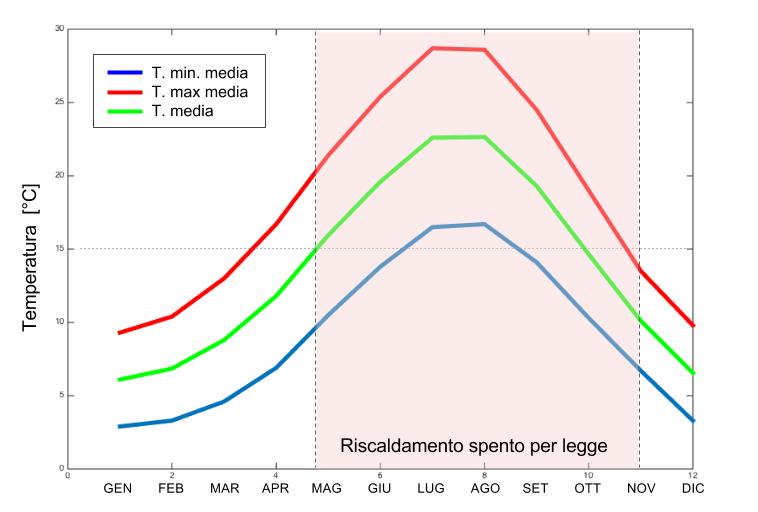
\includegraphics[width=0.95\textwidth]{figure/profilo_temp} 
\caption{Andamento della temperatura minima media, massima media e media durante l'arco di 1 anno nel comune di Pomarance (PI). La zona del grafico evidenziata in rosso rappresenta il periodo in cui per legge il riscaldamento deve essere spento. }
\label{fig:profilo_temp}
\end{figure}

 Il grafico mostra che le temperature più basse rappresentano circa il 5\%. Quindi, se l'impianto di teleriscaldamento è dimensionato per coprire la richiesta massima di energia, vuol dire che nel restante 95\% dell'anno, il sistema risulta sovradimensionato e fornisce più calore del necessario.  Per il 60\% dell'anno il riscaldamento rimane spento per legge (da Maggio fino a Novembre circa) e l'energia termica fornita dall'impianto servirà soltanto per la produzione di acqua igenico sanitaria.

Le utenze hanno bisogno di più calore tanto più la temperatura esterna è bassa. Ciò si verifica perché cresce la differenza di temperatura tra interno ed esterno e di conseguenza aumentano le perdite di calore. 

Generalmente, fornendo una temperatura dell'acqua in uscita dalla centrale costante, la temperatura di ritorno è più alta quando la domanda diminuisce e viceversa.

Uno degli obiettivi principali nella gestione di un sistema di teleriscaldamento è quello  di fornire ai consumatori la corretta quantità di calore secondo le condizioni climatiche esterne,  evitando gli sprechi.

Per controllare al meglio l'impianto si può optare su due diverse soluzioni: la prima consiste nel mantenere la temperatura di mandata dell'acqua costante facendo però variare la portata; l'altra invece mantiene costante il numero di giri della pompa e fa variare la temperatura di mandata dell'acqua. Quest'ultimo metodo è più complicato perché mentre la variazione di portata risulta istantanea, la variazione di temperatura ha bisogno di una certa quantità di tempo  che dipende dalla velocità con cui si propaga l'acqua nella rete, rendendo complicata la gestione in caso di picchi di richiesta di calore. 

Come già citato la potenza termica fornita alle utenze dipende dalla portata e dalla differenza di temperatura tra mandata e ritorno dell'acqua secondo una relazione direttamente proporzionale. Facendo riferimento a regolazioni con pompe a giri variabili, avere una temperatura di ritorno più bassa possibile, permette di ridurre la portata a parità di calore fornito, in quanto aumenta il $\Delta T$, riducendo così i costi di pompaggio.

Per ridurre le perdite di calore invece, è necessario avere una temperatura di mandata più bassa possibile. Il limite minimo di questo parametro è dato dai tipi di impianto che sono installati nelle utenze. I riscaldamenti con radiatori sono i più diffusi, ma sono anche quelli che necessitano una temperatura di funzionamento più alta. Il riscaldamento a pavimento è quello invece che necessita temperature di funzionamento più basse come è mostrato in Figura \ref{fig:elem_scaldanti}. 

Data l'eterogeneità degli impianti di riscaldamento presenti nelle utenze abitative di una normale rete il gestore dovrà garantire una temperatura in mandata che permetta il corretto funzionamento dell'elemento riscaldante che lavora a temperatura più alta.

\begin{figure}[!ht]
\centering
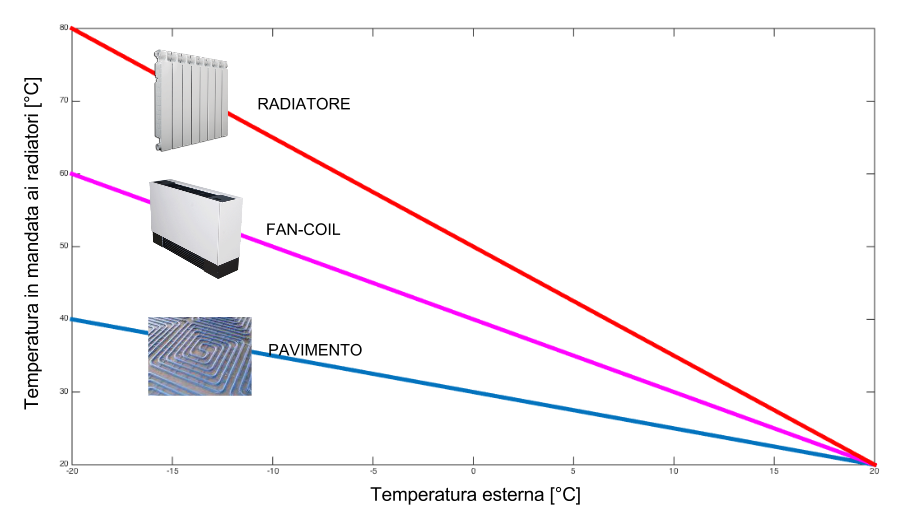
\includegraphics[width=0.85\textwidth]{figure/elem_scaldanti} 
\caption{Temperature di funzionamento di vari tipi di elementi scaldanti al variare della temperatura esterna.}
\label{fig:elem_scaldanti}
\end{figure}

\section{Fabbisogno termico massimale di un'abitazione}
Esiste ovviamente una formula matematica che consente un calcolo approssimativo del fabbisogno termico. Bisogna però tenere presente che è  un risultato indicativo, poiché ci sono moltissime variabili che possono incidere sul reale fabbisogno dell'abitazione, alcune delle quali difficilmente quantificabili. 

Il calcolo matematico fornisce il totale delle kcal necessarie a scaldare l'abitazione utilizzando come dati di partenza
\begin{itemize}
\item  il totale dei metri cubi da scaldare;
\item  un coefficiente termico che indica le calorie necessarie. per metro cubo e che può  oscillare tra un valore che va da 30 a 40 $\frac{Kcal}{m^3}$, a seconda delle condizioni termiche dell'abitazione.
\end{itemize}
Dunque il fabbisogno termico della casa può essere descritto dal prodotto tra il volume dell'utenza per il coefficiente termico scelto in base al tipo di abitazione.

%Questo valore ci da un indice di quanta energia i radiatori dovranno fornire alla casa per scaldarla nelle condizioni climatiche esterne peggiori.


\section{Funzionamento e importanza dell'utilizzo di centraline d'utenza}
\label{sec:centraline}
Le centralina d'utenza rappresenta un elemento di regolazione dell'impianto di teleriscaldamento posizionato nell'abitazione. La centralina è posizionata nella sotto-centrale d'utenza i cui elementi principali sono: uno scambiatore nel caso in cui si utilizzi il teleriscaldamento soltanto per scaldare gli ambienti, o due di essi nel caso si voglia produrre anche acqua calda ad uso sanitario; da una valvola di laminazione a due vie e da una pompa di circolazione. 

In Figura \ref{fig:centralina} è mostrato come si presenta una sotto-centrale con centralina adibita alla produzione combinata del riscaldamento e dell'acqua igenico sanitaria mentre in Figura \ref{fig:schema_centralina2} è rappresentato il suo schema idraulico.

\begin{figure}[!ht]
\centering
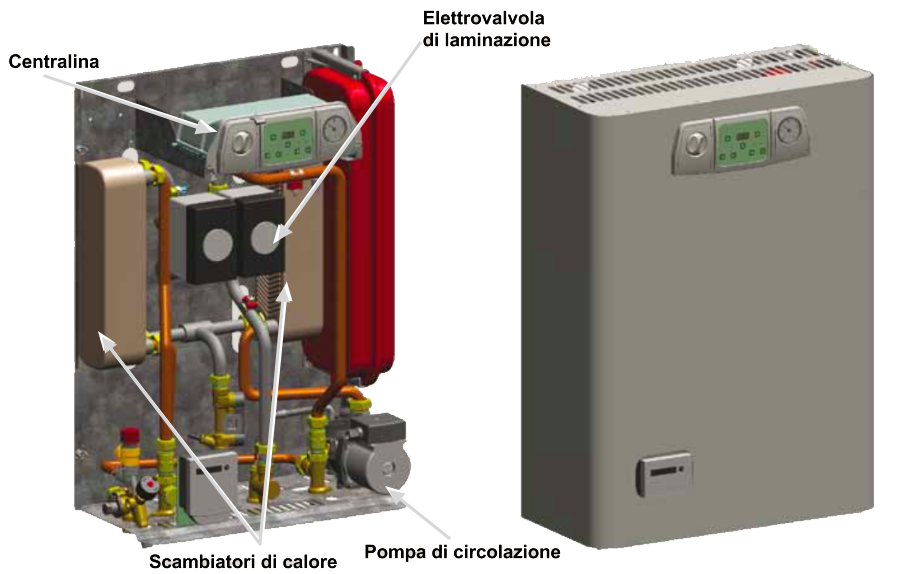
\includegraphics[width=0.95\textwidth]{figure/centralina} 
\caption{Sottostazione d'utenza con centralina.}
\label{fig:centralina}
\end{figure}

\begin{figure}[!ht]
\centering
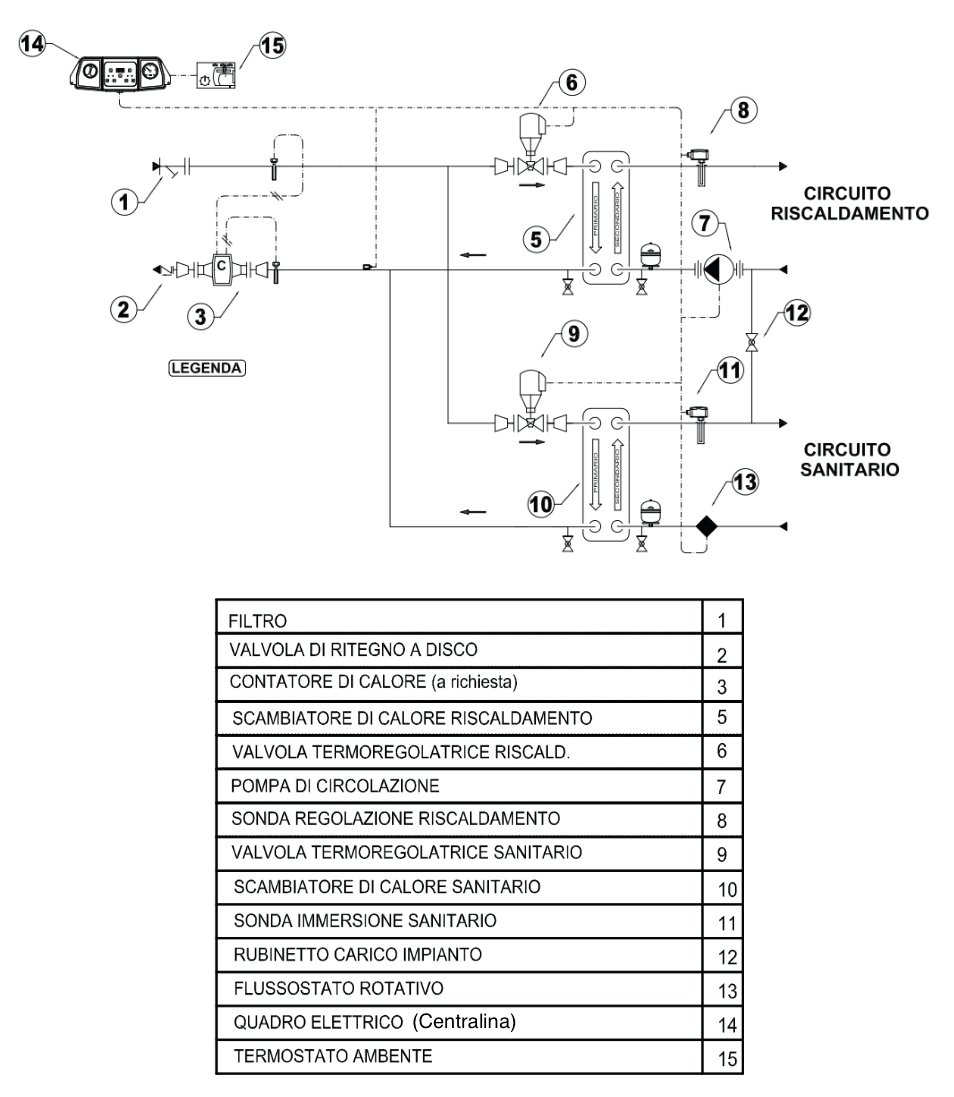
\includegraphics[width=\textwidth]{figure/schema_centralina2} 
\caption{Schema idrico di una sottostazione d'utenza con centralina.}
\label{fig:schema_centralina2}
\end{figure}

Si tratta di una sotto-centrali compatte appositamente studiate e progettate con dimensioni pari ad una caldaia tradizionale.
Il comando di accensione del circuito riscaldamento avviene dal cronotermostato ambiente. Durante il funzionamento in riscaldamento la temperatura di mandata dell'acqua all'impianto potrà essere liberamente modificata in base al tipo di regolazione installata. Il controllo  avviene direttamente sul circuito primario tramite la valvola termoregolatrice a due vie.
Il funzionamento sanitario si attiva attraverso il flussostato in modalità prioritaria o parallela; la regolazione modulerà la valvola termoregolatrice primaria per erogare l’acqua sanitaria alla temperatura desiderata.

Il grado di chiusura della valvola di laminazione è determinato da una centralina in base al criterio di controllo scelto. Le regolazioni che possono essere implementate sono le seguenti e verranno approfondite in seguito:

\begin{itemize}
\item regolazione a punto fisso;
\item termoregolazione climatica;
\item regolazione climatica evoluta PI.
\end{itemize}  

In Figura \ref{fig:schema_centralina} è  rappresentato lo schema che mostra quali sono gli ingressi e le uscite della centralina.

\begin{figure}[!ht]
\centering
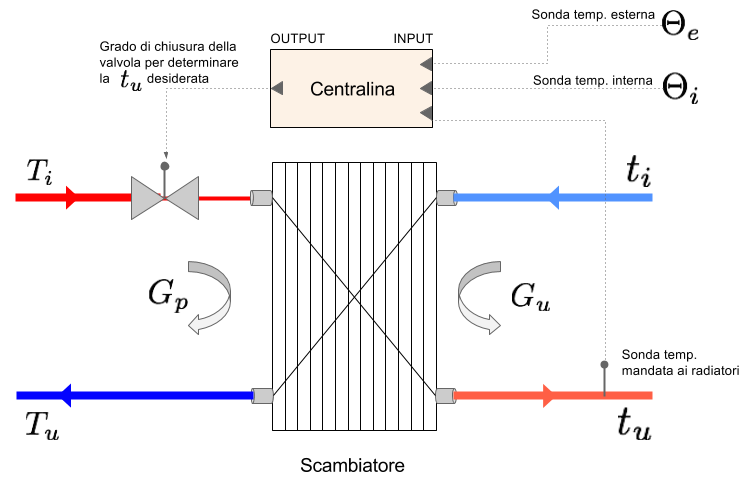
\includegraphics[width=0.95\textwidth]{figure/schema_centralina} 
\caption{Schema dei possibili input e output di una centralina installata su una sottostazione d'utenza}
\label{fig:schema_centralina}
\end{figure}


Le sottostazioni d'utenza con centralina, e quindi con regolazione della portata in ingresso allo scambiatore, devono permettere anche un'analisi di predittiva sullo stato di funzionamento degli scambiatori con segnalazione di anomalie che portano ad interventi programmati invece che in accidentale, il tutto per avere un sistema sempre funzionante al massimo dell'efficienza.

Di notevole importanza è la possibilità che le centraline delle utenze più svantaggiate (ovvero quelle che hanno la portata più bassa nel sistema), oppure quelle di tutte le utenze se la rete è di piccole dimensioni, comunichino informazioni alla stazione di pompaggio per ottimizzare la portata delle pompe e garantire a tutte le utenze il necessario flusso di acqua per il proprio fabbisogno. Attualmente gli unici sensori di pressione e misuratori di portata esistenti nell'impianto sono posizionati nella centrale di scambio. Questo posizionamento non è il più conveniente. Infatti, è possibile misurare se viene raggiunta una certa differenza di pressione tra mandata e ritorno ma non sapremo se tale valore  è sufficiente al passaggio di acqua negli scambiatori delle utenze più svantaggiate. Attualmente, eventuali carenze di pressione e/o portata sono comunicate direttamente dagli utenti perché sentono i radiatori freddi.

Riassumendo, i sistemi di regolazione delle centraline d'utenza devono:
\begin{itemize}
\item controllare che i flussi nello scambiatore siano quelli ottimali, limitando la portata secondo la regolazione più opportuna;
\item controllare che nello scambiatore vi sia il massimo abbattimento di temperatura possibile, evitando che circoli inutilmente acqua calda;
\item aiutare a fare efficienza al cliente finale, utilizzando la termoregolazione climatica che definisce il carico termico massimo da fornire all'utenza in base alla temperatura esterna;
\item permettere al gestore di avere utili indicazione per interventi manutentivi come nel caso di intasamento degli scambiatori oppure una bassa differenza di pressione ai capi dello scambiatore;
\item almeno le centraline dei punti più svantaggiati devono fornire informazioni per ottimizzare i consumi delle pompe.
\end{itemize}

\section{Soluzioni per aumentare l'efficienza delle utenze diminuendo la temperatura dell'acqua di ritorno}
Nonostante i problemi che comportano le reti di distribuzione senza regolazioni di portata in arrivo alle utenze, sono ancora molte le abitazioni che ne sono prive.
Dettò ciò andremo a studiare alcuni tipi di regolazioni che aumentino l'efficienza delle abitazioni. 
Come base di paragone per tutte le simulazioni future verrà preso in considerazione uno scambiatore senza limitatore di portata: tutto il flusso di acqua in arrivo allo scambiatore verrà utilizzato per fornire calore all'acqua del circuito dell'utenza. 
L'analisi è stata effettuata  simulando i diversi scenari esaminando quali di questi permettono di ottenere una portata e una temperatura di ritorno dell'acqua più bassa.

Tutte le simulazioni di questo paragrafo si riferiscono ad un'abitazione con temperatura interna desiderata impostata a $20 ^{\circ}$C con le seguenti caratteristiche (le variabili che andremo a definire sono descritte nel capitolo 3):\\
\textbf{parametri abitazione }
\begin{itemize}
\item[] Volumetria 300 $m^3$: abitazione di 100 $m^2$ con pareti alte 3 $m$
\item[] $C_a = M_a \cdot c_a$ = $2487 \ kcal/^{\circ}$C (in questo prodotto oltre che considerare la massa e il calore specifico dell'aria, vi è sommato anche la massa delle pareti interne alla casa che formano le stanze e il loro calore specifico. Infatti, queste pareti assorbono molta energia e giocano un ruolo fondamentale per ottenere in simulazione un andamento realistico della temperatura interna dell'utenza)

\item[] $C_p = M_p \cdot c_p =12629 \ kcal/^{\circ}$C con:\\
 $\ \cdot \ M_p$ = 62725 $kg$ : pareti composte da due strati:
\begin{itemize}
\item[] Muratura in laterizi forati (10 cm di spessore): $M_{p1}$ = 19630 $kg$
\item[] Termolaterizio POROTON (20 cm di spessore): $M_{p2}$ = 42884 $kg$ 
\end{itemize}
$\ \cdot \ c_p$ = 0,80 $kcal/kg \cdot ^{\circ}$C: pareti composte da due strati:
\begin{itemize}
\item[] Muratura in laterizi forati (10 cm di spessore): $c_{p1}$ = 0,20 $kcal/kg \cdot ^{\circ}$C
\item[] Termolaterizio POROTON (20 cm di spessore): $c_{p2}$ = 0,20 $kcal/kg \cdot ^{\circ}$C
\end{itemize}

\item[] $R_{ip}^{-1}$ = $1996 \ kcal/ ^{\circ}$C
\item[] $R_{pe}^{-1}$ = $129.86 \ kcal/ ^{\circ}$C
\item[] $R_{f}^{-1}$ = $114.53 \ kcal/ ^{\circ}$C
\end{itemize}

\textbf{paramentri radiatore}
\begin{itemize}
\item[]$Km = 51,5 \ kcal/^{\circ}$C  
\item[]$n = 1,32$
\item[]$G_p = 600 \ l/h$
\end{itemize}

\textbf{parametri scambiatore}
\begin{itemize}
\item[]$\alpha \cdot S = 900 \ kcal / ^{\circ}$C
\item[]$T_i = 82 \ ^{\circ}$C
\end{itemize}

\textbf{parametri iniziali}
\begin{itemize}
\item[]$\Theta_i(0) = 18 \ ^{\circ}$C
\item[]$\Theta_p(0) = 15 \ ^{\circ}$C
\end{itemize}

\textbf{parametri esterni}
\begin{itemize}
\item[] La temperatura esterna $\Theta_e$ segue il profilo illustrato in Figura \ref{fig:temp_est} che mostra l'andamento di temperatura giornaliero (24 ore) in una giornata invernale dalle 8:00 del mattino fino alla stessa ora del giorno successivo. 
\end{itemize}

Il parametro $M_a$ oltre che

\begin{figure}[!h]
\centering
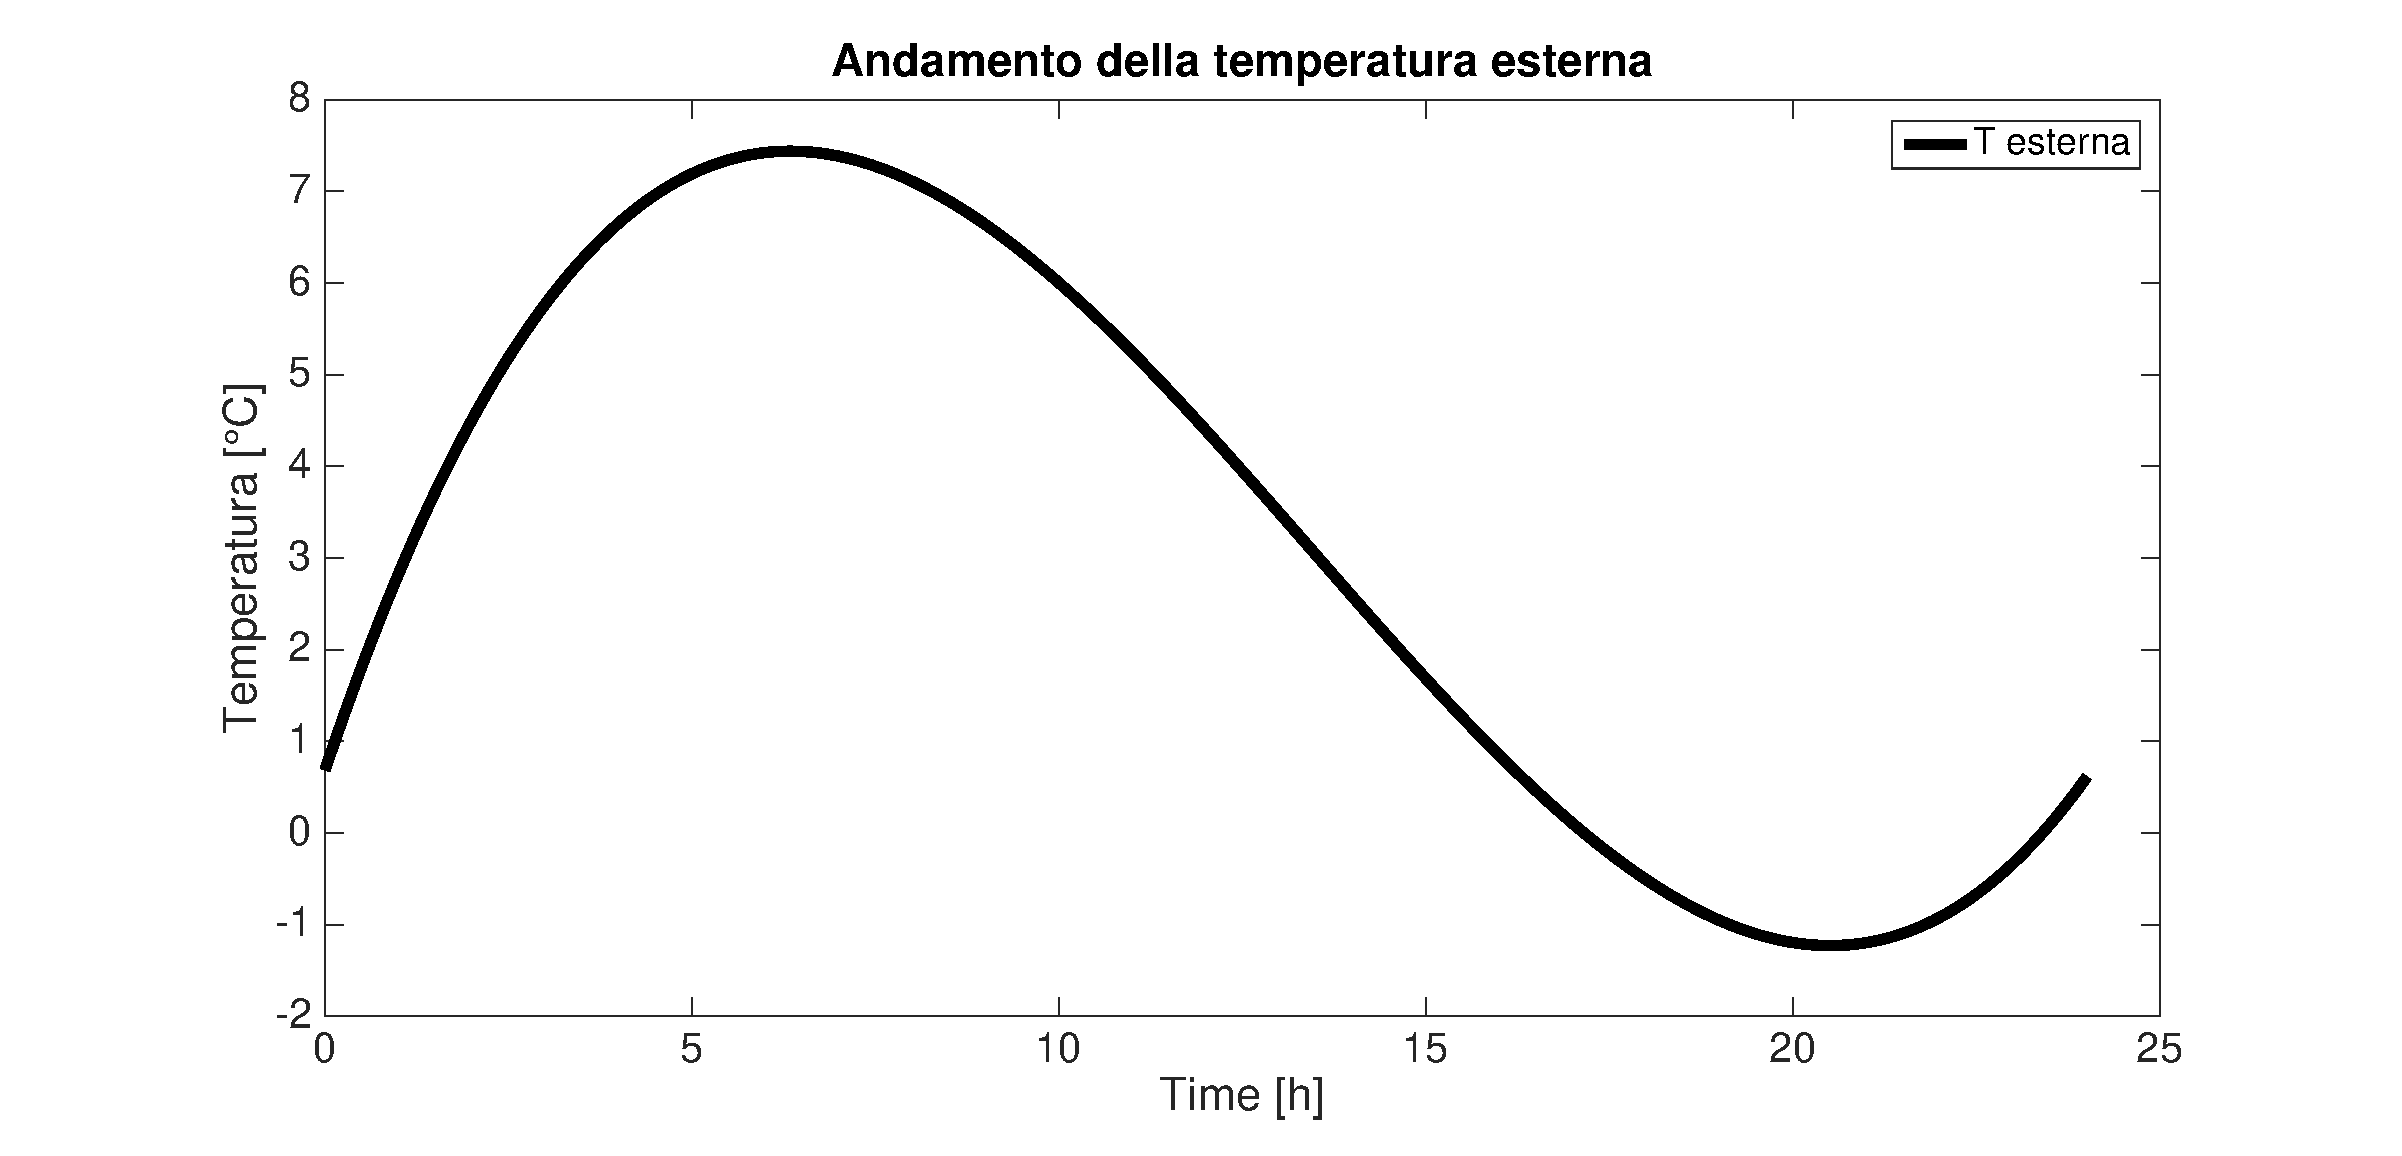
\includegraphics[width=\textwidth]{figure/temp_est} 
\caption{Andamento della temperatura esterna per 24h in una giornata invernale}
\label{fig:temp_est}
\end{figure}

Per convenzione quando la pompa di utenza è spenta le temperature $t_u$ e $t_i$ vanno a zero per indicare che non vi è scambio di calore con i radiatori. Nel caso di sottostazioni con regolazione anche $T_i$ e $T_u$ quando vanno a zero indica che la valvola di laminazione è completamente chiusa e non è quindi permesso il passaggio di acqua. 

%La regolazione dell'impianto può seguire due principi: a punto fisso, cioè con temperatura di mandata fissata indipendentemente dalle condizioni esterne; climatica, cioè con adeguamento continuo alla situazione di temperatura esterna. La climatica del futuro ormai prossimo, sarà una regolazione evoluta, che ottimizza i consumi in funzione del comfort, tutto questo sarà possibile grazie all'algoritmo PI.
\subsection{Regolazione di portata assente}
In Figura \ref{fig:no_reg} è mostrato l'andamento della temperatura ambiente $\Theta_i$, delle temperature $T_i, T_u, t_u, t_i$ dello scambiatore e la portata nel caso di un'utenza che dispone di uno scambiatore senza alcun tipo di regolazione sulla portata in ingresso. La temperatura è impostata sul termostato a 20 $^{\circ}$C mentre la portata $G_p$ è di 1500 $l/h$ (si considera un utenza posta nelle vicinanze della centrale di scambio che quindi dispone di una portata abbastanza elevata). 

\begin{figure}[!ht]
\centering
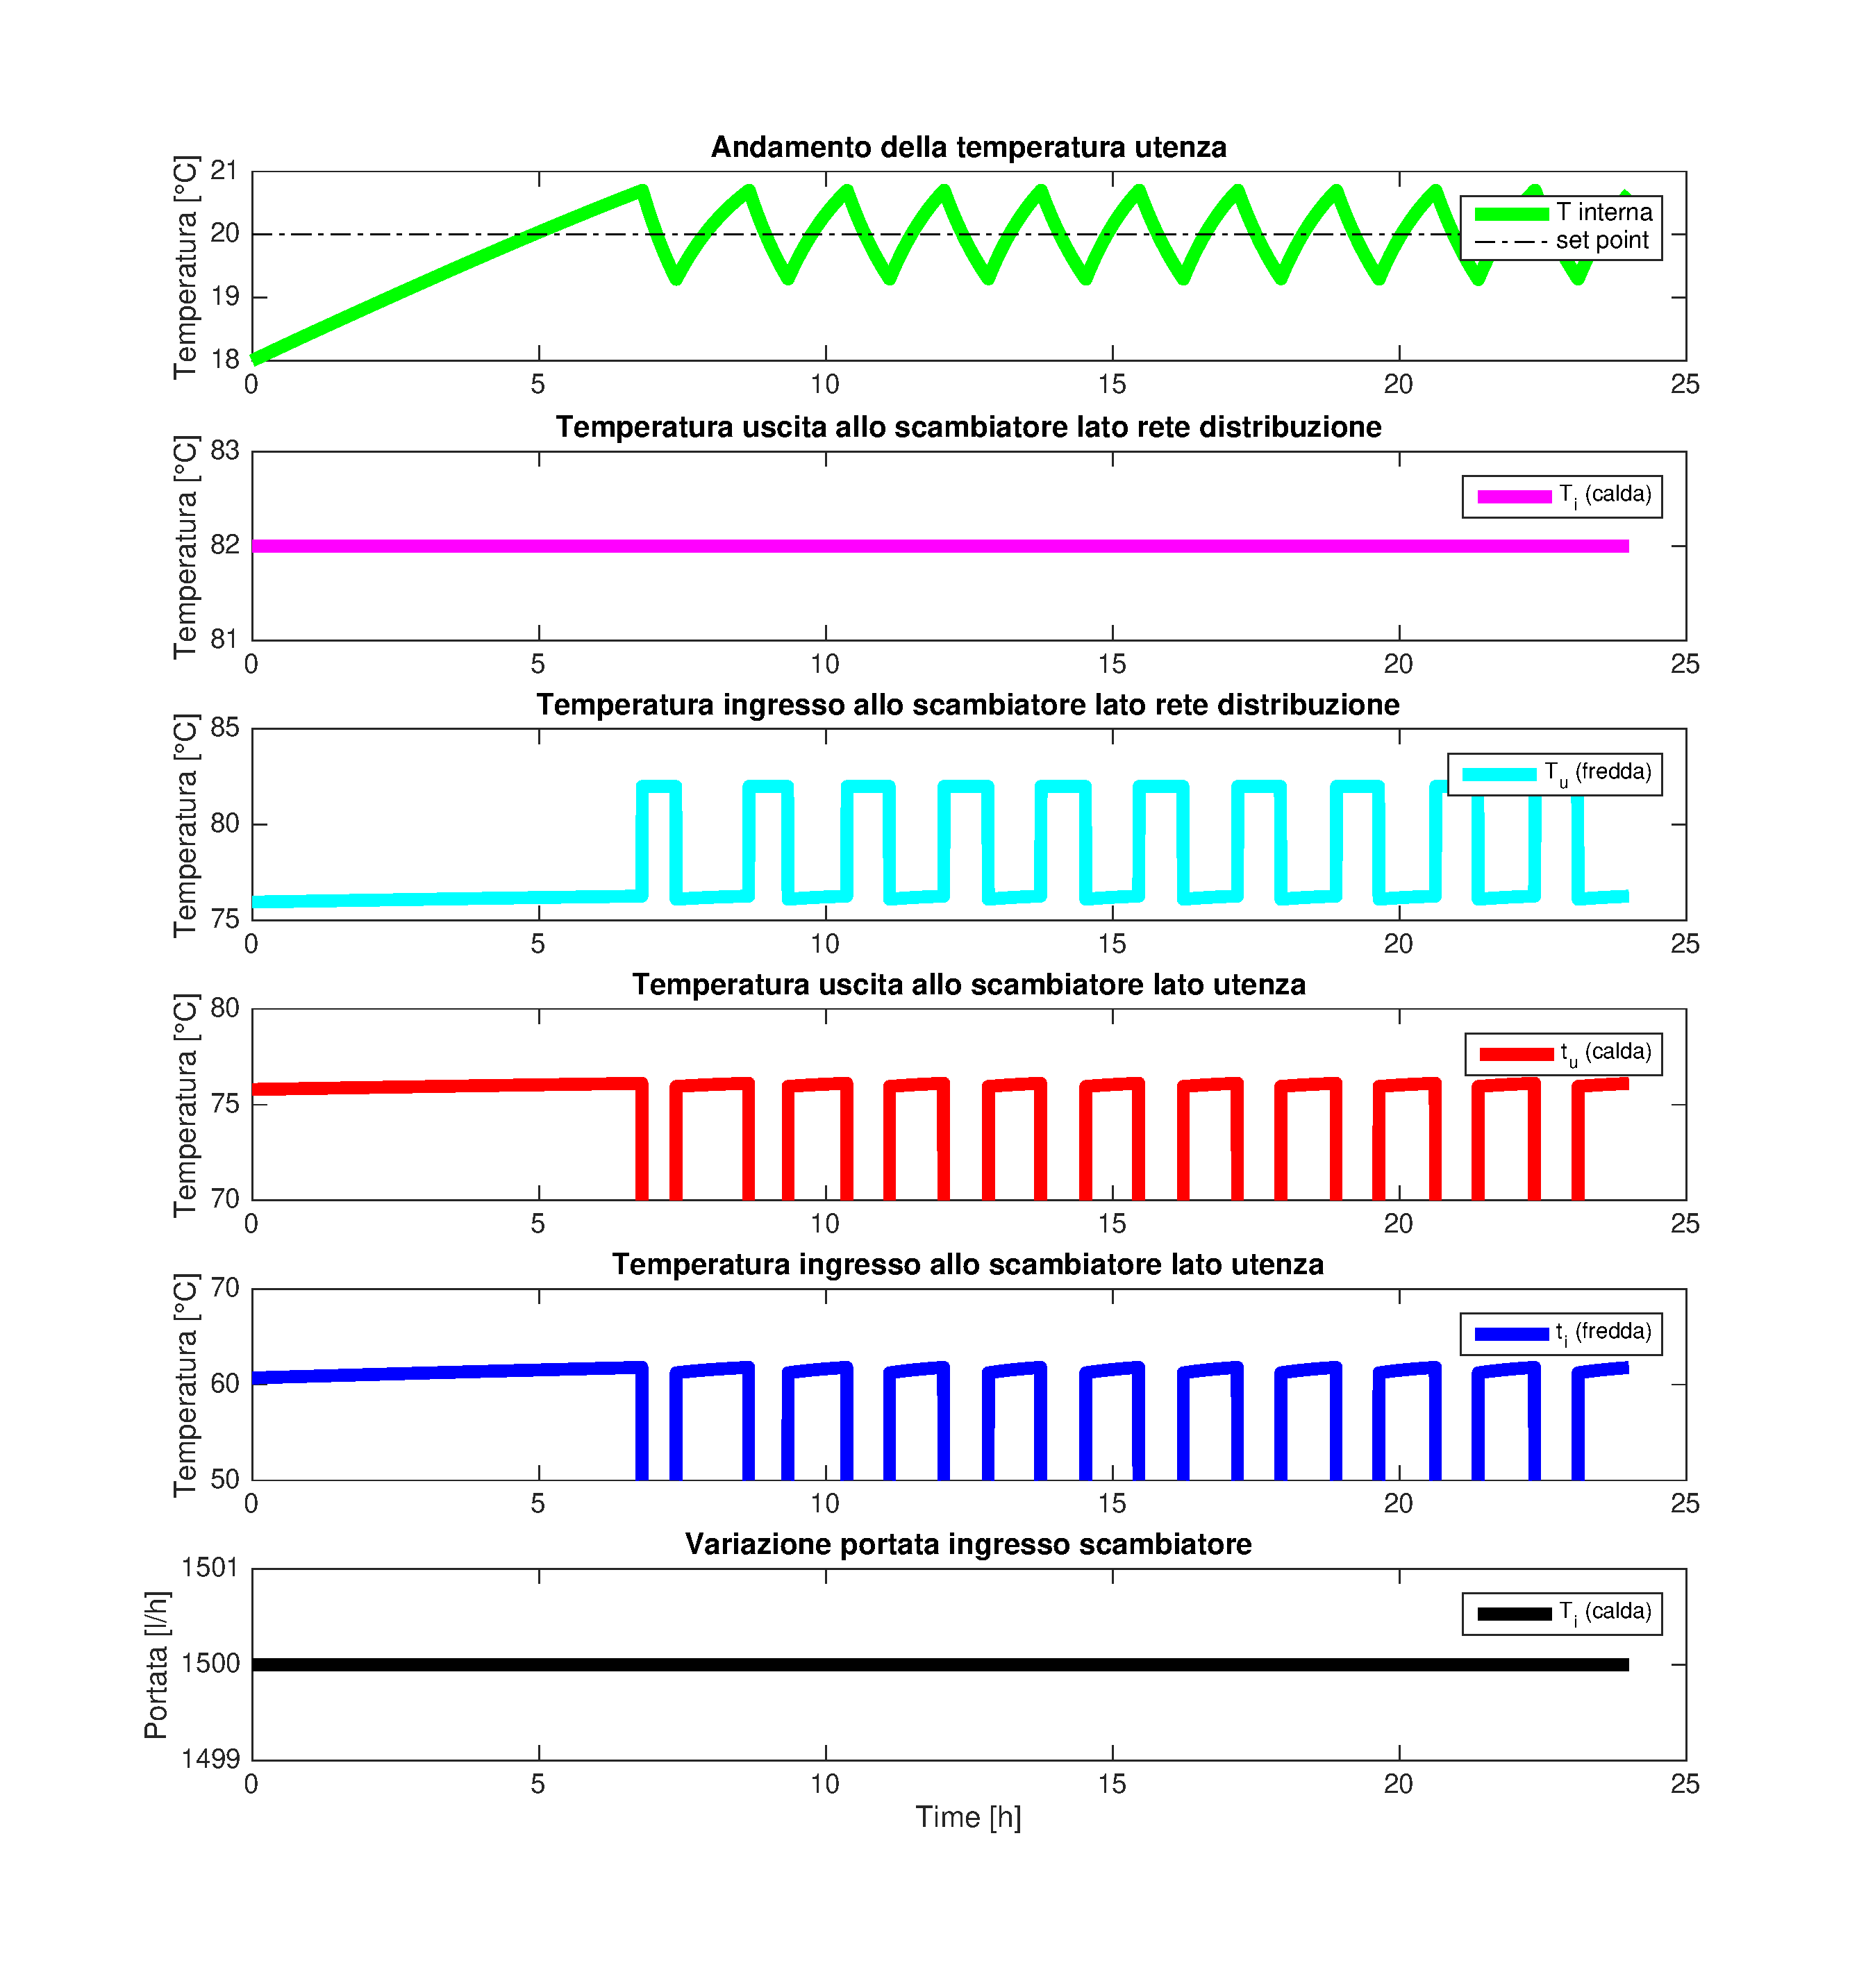
\includegraphics[width=\textwidth]{figure/no_reg} 
\caption{Andamento della temperatura ambiente, delle temperature $T_i, T_u, t_u, t_i$  dello scambiatore e la portata per una sotto-centrale senza regolazioni sulla portata.}
\label{fig:no_reg}
\end{figure}

Con questa configurazione quando si raggiunge la temperatura di set-point si spegne la pompa così da terminare lo scambio di calore. La pompa si riattiverà quando viene misurata una temperatura ambiente troppo bassa. Quando la pompa d'utenza è spenta, l'acqua calda $T_i$ in ingresso allo scambiatore non scambia calore, e la temperatura di uscita $T_u$ sarà più o meno uguale a $T_i$. Questo vale a dire che la temperatura di ritorno sarà molto alta e il sistema risulterà inefficiente perché utilizziamo energia elettrica per pompare acqua calda senza che vi sia alcuno scambio di energia termica.

%valutare se inserire una Tabella con dati di altre simulazioni

\subsection{Termoregolazione a punto fisso}
Si tratta del sistema di regolazione più semplice. La regolazione a punto fisso garantisce all'impianto una temperatura del fluido di mandata costante. 

Il valore viene impostato manualmente attraverso una valvola termostatica che regola la portata in ingresso allo scambiatore.  

Il limite maggiore è la necessità, da parte dell'utilizzatore, di dover regolare l'impianto ogni volta che variano le condizioni esterne. Per ridurre questa esigenza si è diffusa la consuetudine di tarare la valvola termostatica sulla temperatura di progetto, uguale alla massima temperatura necessaria nel giorno più freddo dell'anno. In questo modo però nei giorni meno freddi si avrà un surplus di energia che riduce l'efficienza dell'abitazione.

Il termostato confronta la temperatura impostata dall'utilizzatore con quella presente e, se la temperatura in ambiente supera quella impostata, toglie corrente alla pompa di circolazione e chiude la valvola di laminazione, interrompendo il flusso di acqua nello scambiatore d'utenza. 

Quando la temperatura in ambiente è scesa fino ad essere inferiore a quella richiesta, il termostato comanda la riapertura, in modo da garantire nuovamente la temperatura ideale.

\begin{figure}[!ht]
\centering
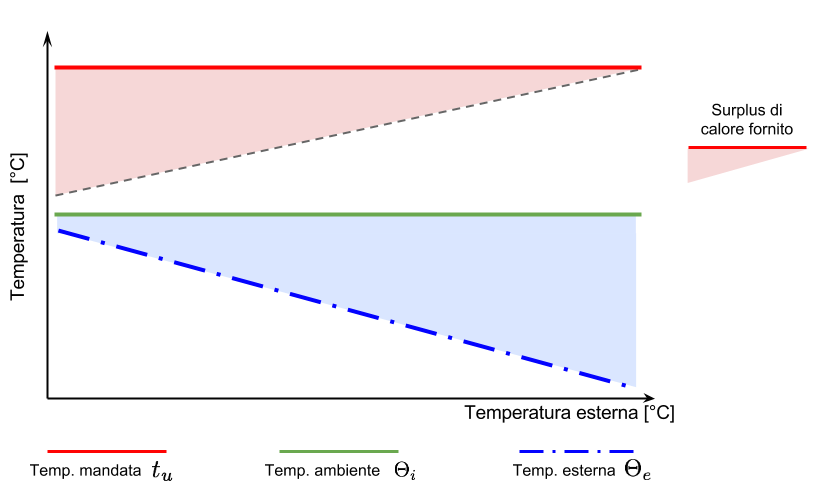
\includegraphics[width=0.85\textwidth]{figure/surplus} 
\caption{Nella regolazione a punto fisso l'acqua circola alla temperatura corrispondente al valore necessario per il giorno più freddo dell'inverno. Nel grafico sono mostrati i surplus di energia in funzione della temperatura esterna.}
\label{fig:surplus}
\end{figure}

In Figura \ref{fig:reg_mandata} viene mostrato come si comporta uno scambiatore con regolazione di mandata a punto fisso. La temperatura di mandata ai radiatori $t_u$ è impostata a 70  $^{\circ}C$.  

\begin{figure}[!ht]
\centering
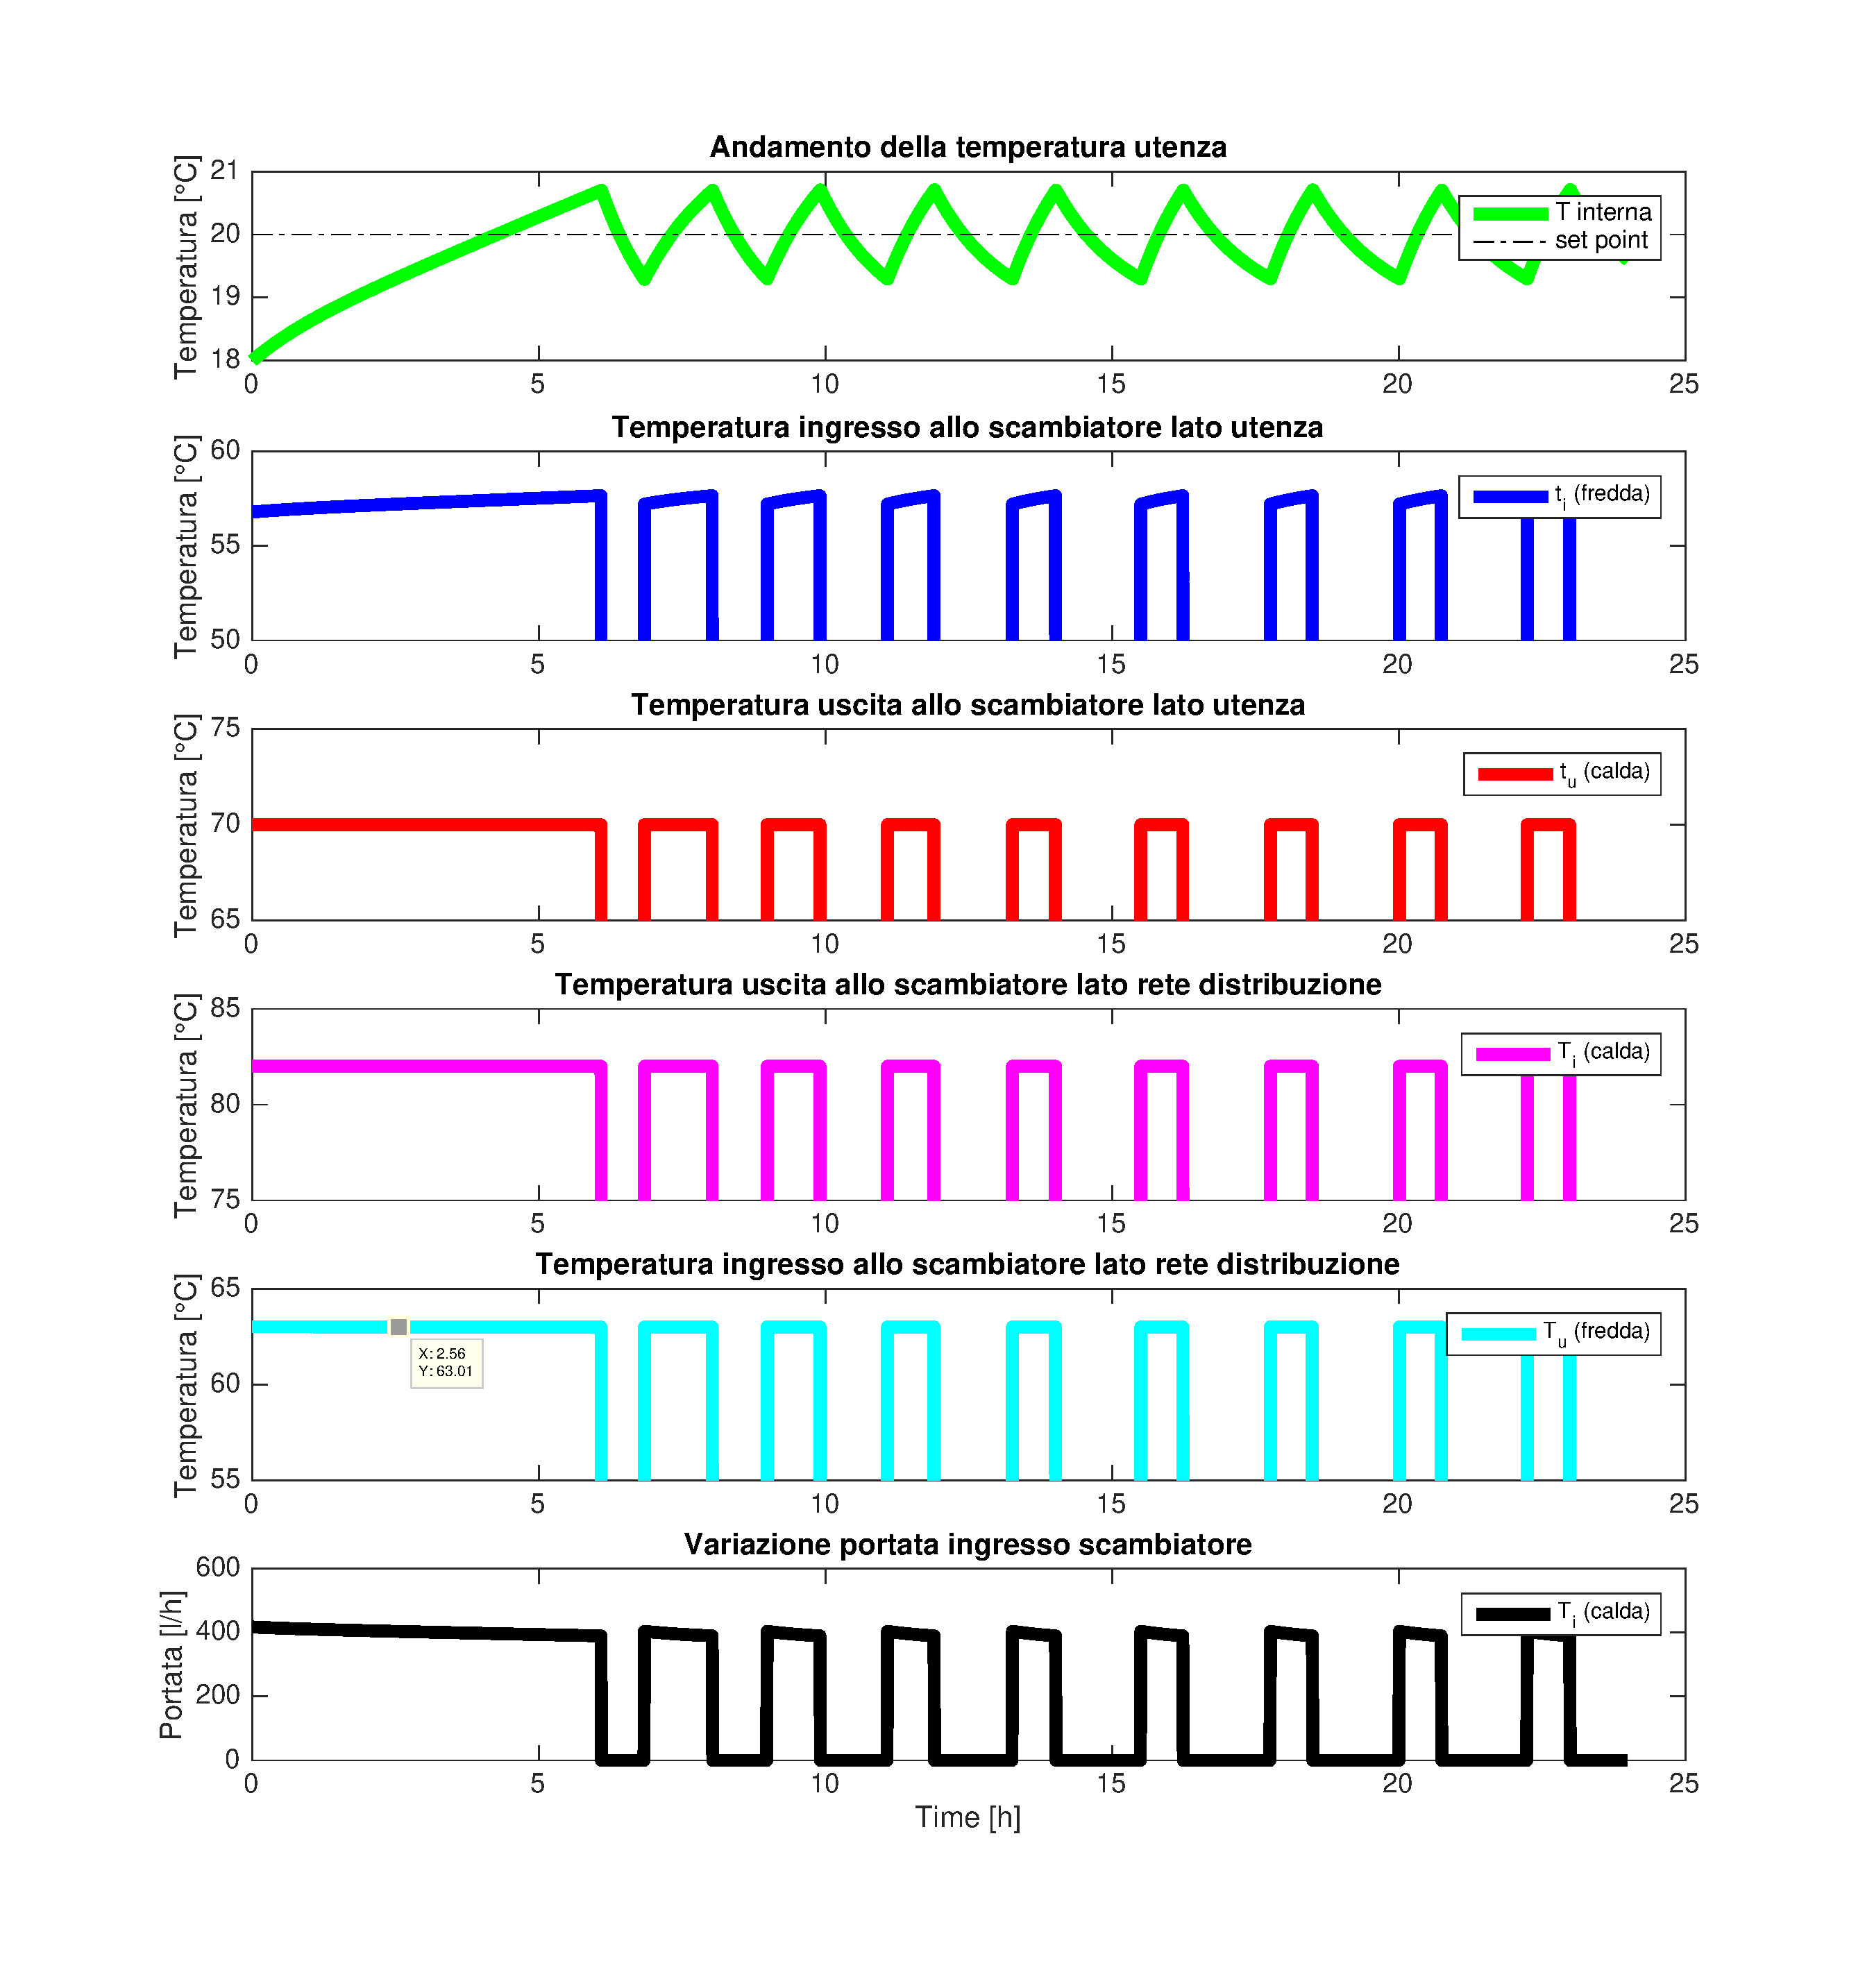
\includegraphics[width=\textwidth]{figure/reg_mandata} 
\caption{andamento della temperatura interna $\Theta_i$, delle temperature $T_i, T_u, t_u, t_i$ dello scambiatore e la portata per una sotto-centrale con termoregolazione a punto fisso.}
\label{fig:reg_mandata}
\end{figure}

Quando il termostato spegne il riscaldamento, la valvola di laminazione si chiude impedendo che vi sia un ritorno di acqua calda alla centrale. Inoltre rispetto al caso di scambiatore senza regolazione la temperature di ritorno $T_u$ risulta più bassa.


\subsection{Termoregolazione climatica}
Poiché il calore necessario per mantenere le condizioni di comfort in ambiente è legato alle dispersioni dell'edificio ed alla temperatura esterna, il fabbisogno termico aumenta all'aumentare delle dispersioni dell'edificio e al diminuire della temperatura esterna. Le regolazioni di tipo climatico permettono di selezionare una curva climatica all'interno di una famiglia di curve, in modo da adeguare la regolazione allo specifico edificio. 

Fissata la curva climatica, la temperatura di mandata all'impianto viene regolata in modo automatico in funzione della temperatura esterna, adeguando l'apporto di calore al fabbisogno termico dell'edificio, per garantire sempre le migliori prestazioni in termini di comfort. 

\begin{figure}[!ht]
\centering
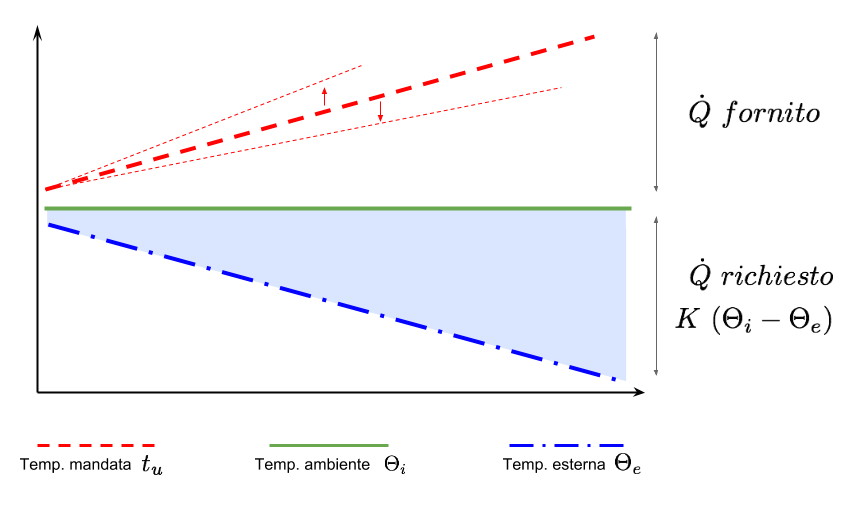
\includegraphics[width=0.85\textwidth]{figure/climatica} 
\caption{La regolazione climatica regola la temperatura di mandata in funzione del calore necessario (funzione della temperatura esterna) e la pendenza della $t_u$ mandata dipende dal fabbisogno termico dell'edificio}
\label{fig:surplus}
\end{figure}

Per ottenere questi risultati si utilizza una centralina elettronica digitale, a cui sono collegate due sonde di temperatura: una inserita nella condotta di mandata ai radiatori e una esterna. 

La centralina elabora il segnale della sonda esterna e in base al codice climatico più adatto per quel tipo di edificio, determina il valore ideale della temperatura di mandata, lo confronta con il valore reale misurato dalla sonda e, se necessario, agisce sull'elettrovalvola posizionata nella condotta in ingresso allo scambiatore per regolare la portata di acqua calda.

La curva climatica o curva di riscaldamento è il rapporto tra la temperatura esterna e la temperatura di mandata ai corpi scaldanti. Per un corretto dimensionamento di tale curva si necessita la conoscenza di due parametri:
\begin{itemize}
\item Temperatura esterna minima di progetto
\item Temperatura massima di mandata all'impianto di riscaldamento
\end{itemize}

%Per questo tipo di regolazione si deve definire una curva di compensazione la quale descrive in base alla temperatura esterna, misurata da una sonda, quale dovrà essere la temperatura in mandata ai radiatori.
La curva deve garantire una temperatura interna alla casa teorica di 20 $^{\circ}$C  per temperature esterne comprese tra $+20$ $^{\circ}$C e $-20$ $^{\circ}$C. La curva  utilizzata per questa simulazione è rappresentata in Figura \ref{fig:curva_comp}.
 
 \begin{figure}[!ht]
\centering
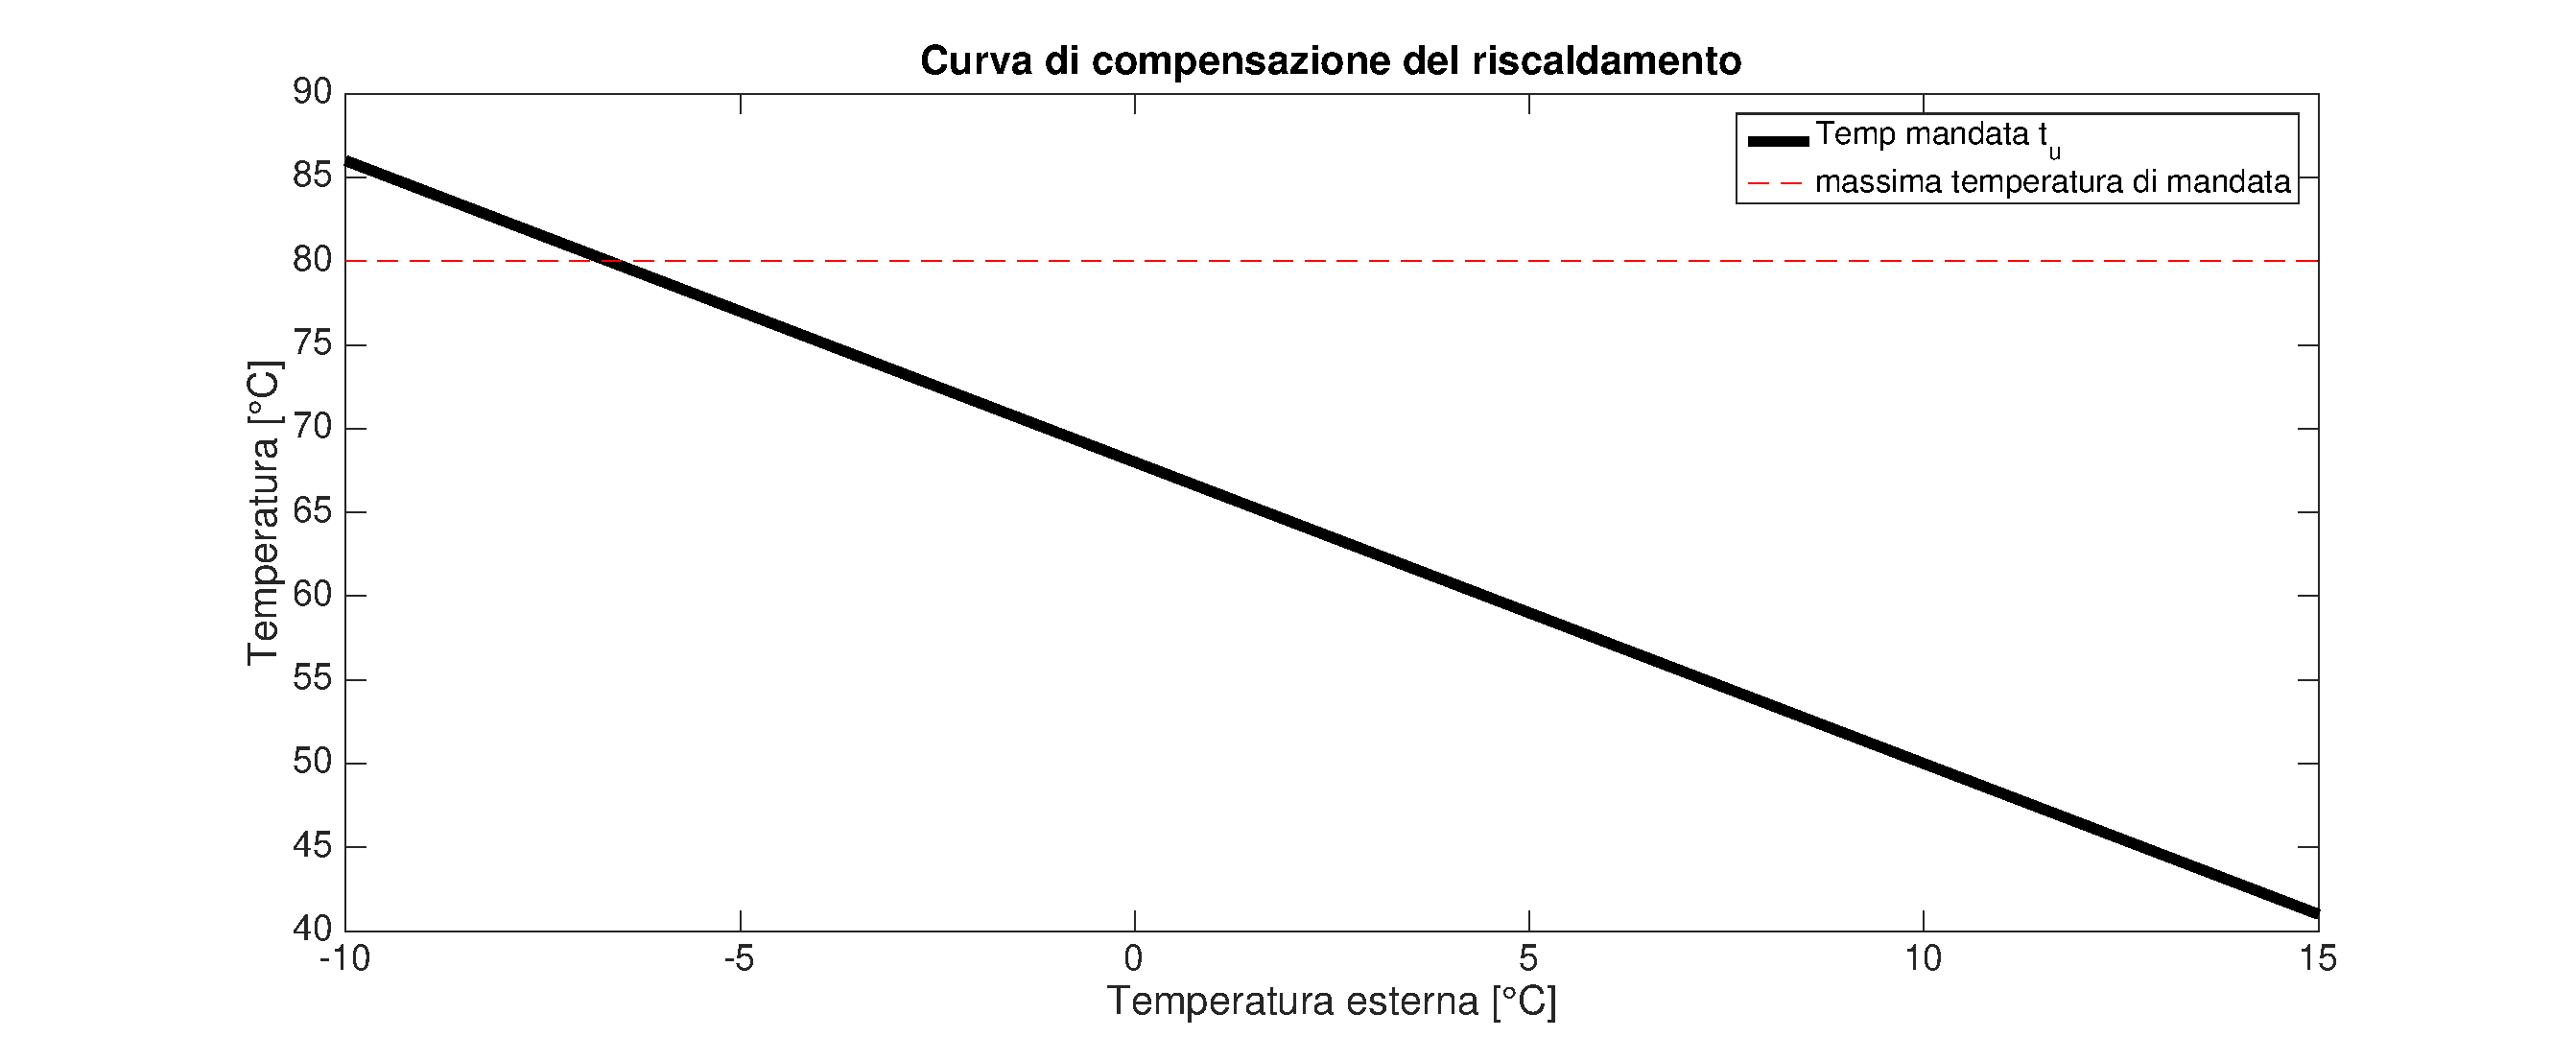
\includegraphics[width=\textwidth]{figure/curva_comp} 
\caption{Curva di compensazione del riscaldamento.}
\label{fig:curva_comp}
\end{figure}


In Figura \ref{fig:reg_climatica} è mostrato l'andamento della temperatura interna $\Theta_i$, delle temperature $T_i, T_u, t_u, t_i$ dello scambiatore e la portata.

\begin{figure}[!ht]
\centering
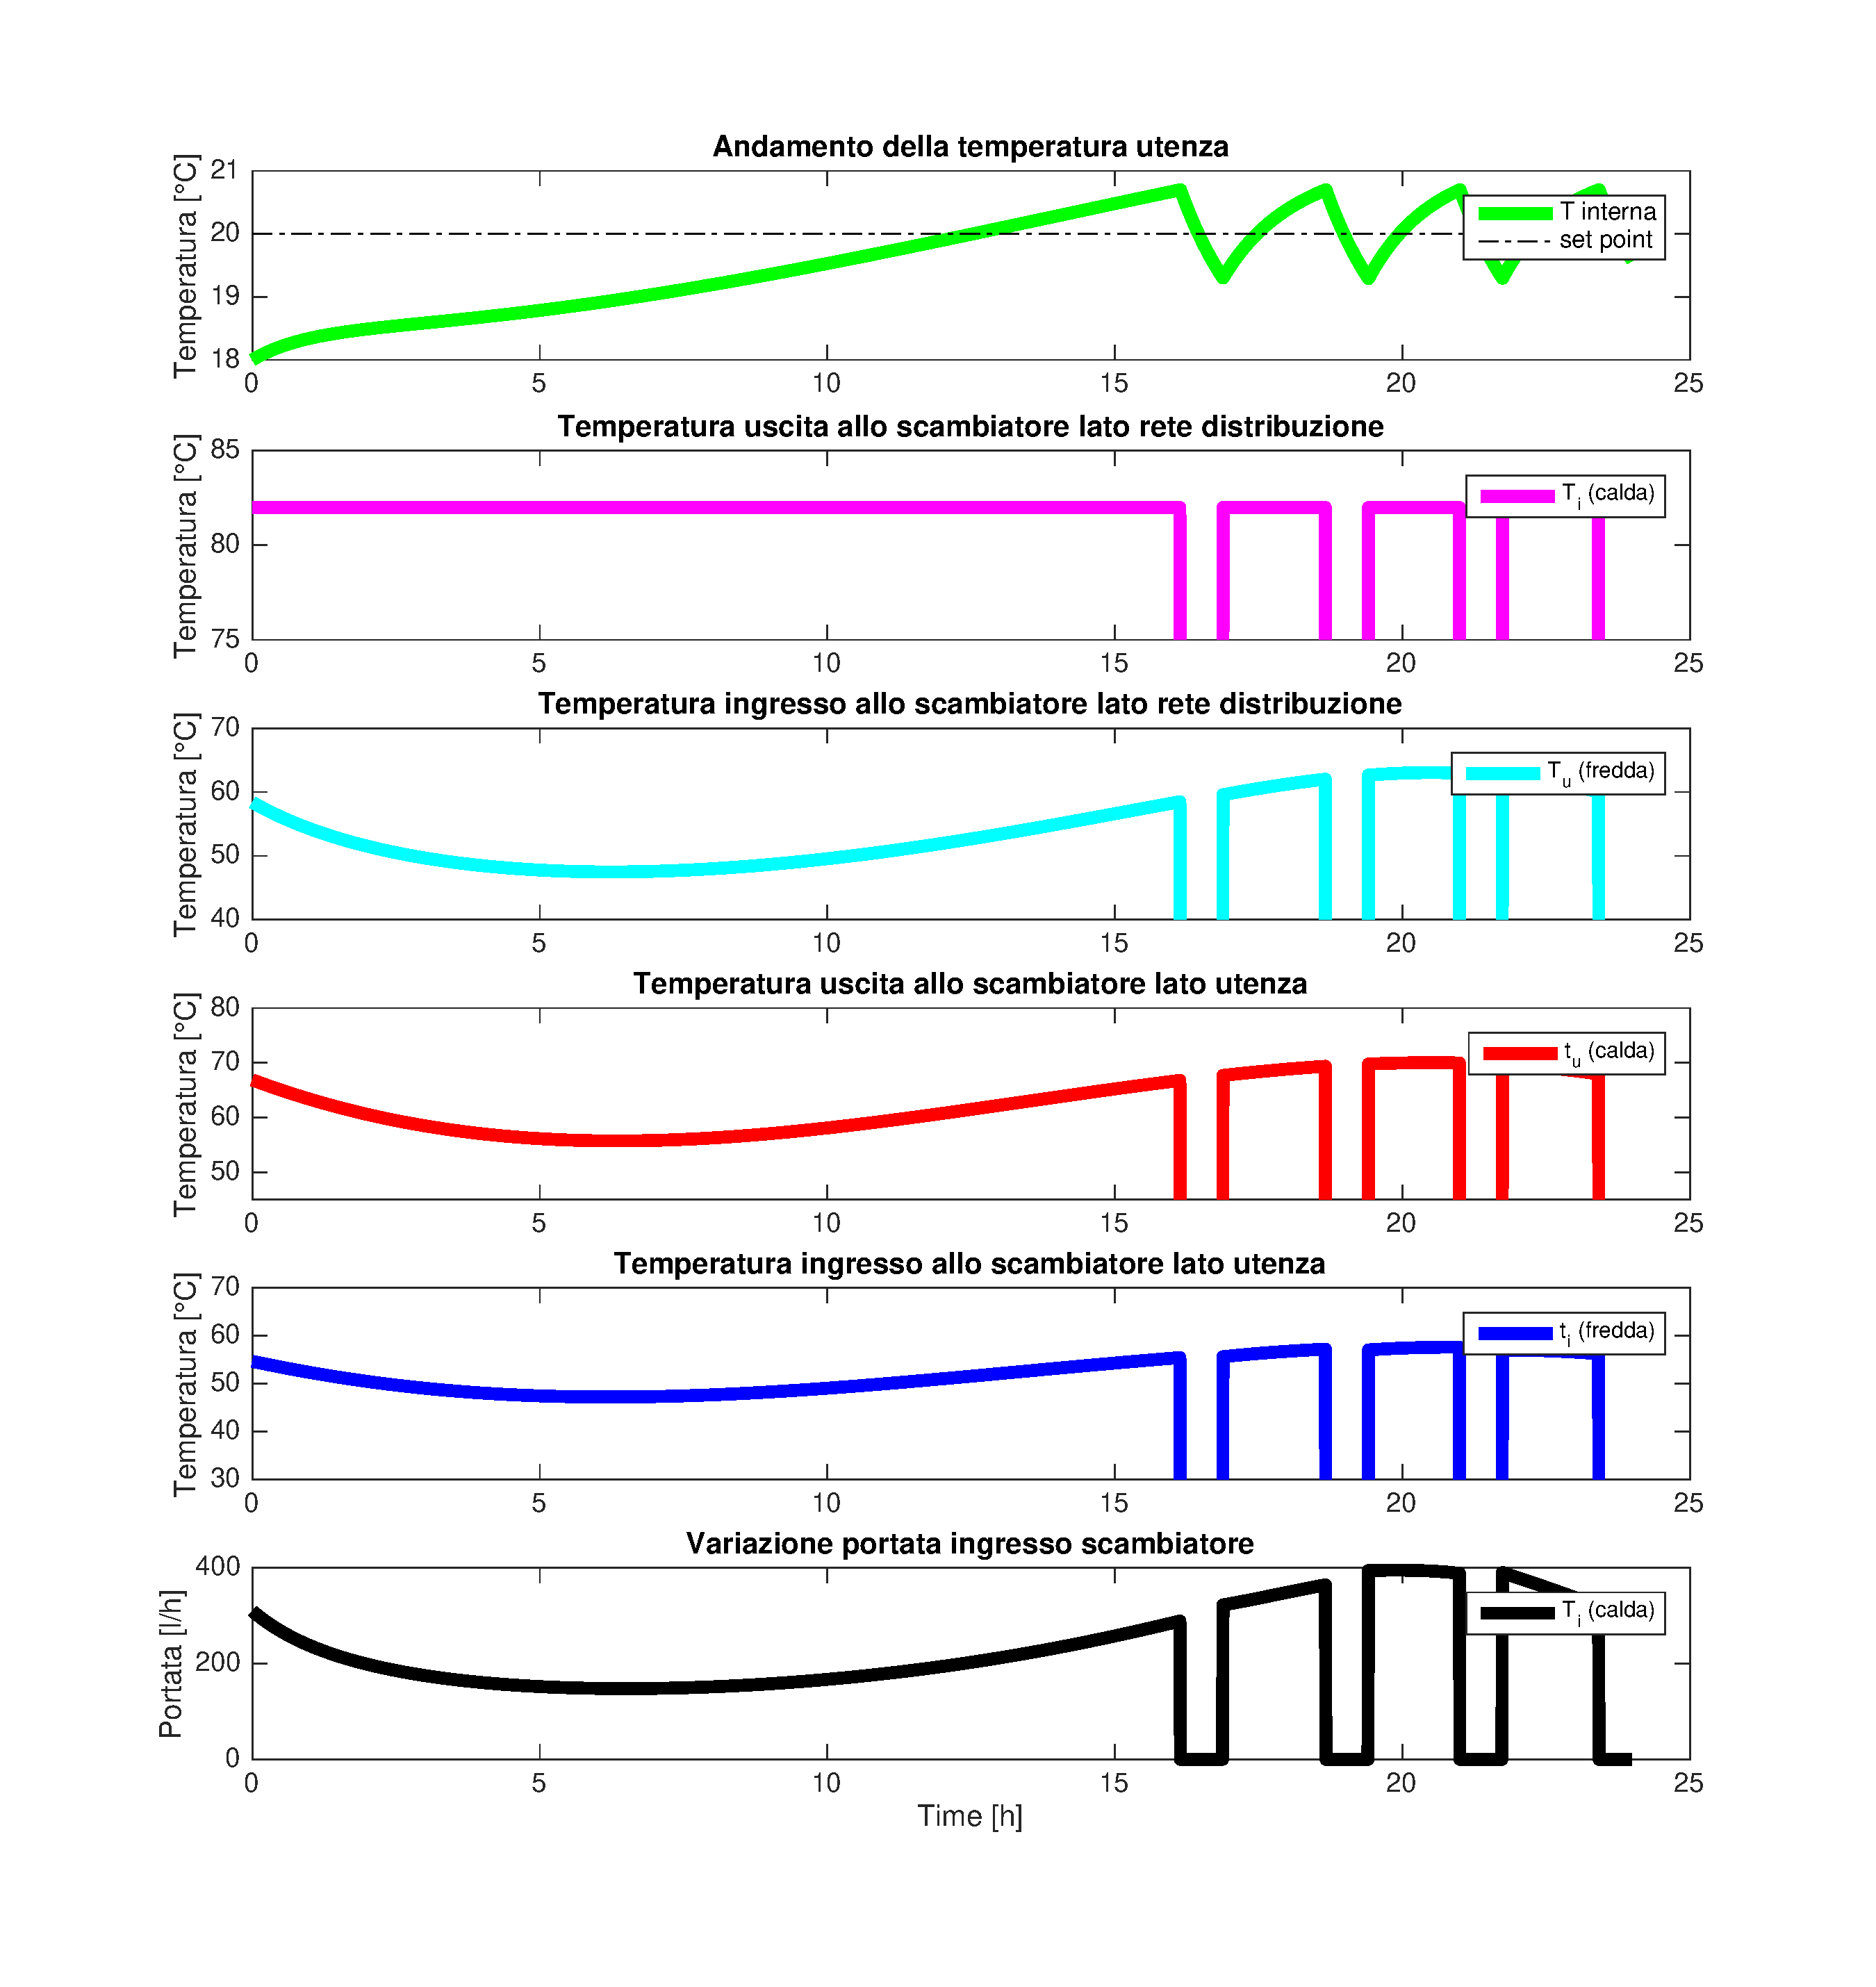
\includegraphics[width=\textwidth]{figure/reg_climatica} 
\caption{Andamento della temperatura interna $\Theta_i$, delle temperature $T_i, T_u, t_u, t_i$ dello scambiatore e la portata per una sotto-centrale con termoregolazione climatica.}
\label{fig:reg_climatica}
\end{figure}

Ben si nota come le temperatura di ritorno $T_u$ e le portate più basse  $G_p$ si hanno quando la temperatura esterna è più alta. Questo indica che non è fornito un surplus di energia riuscendo comunque a raggiungere il livello di comfort desiderato.

\subsection{La regolazione climatica evoluta PI}
Una regolazione climatica evoluta è in grado di gestire in modo ottimale il comfort indoor per quanto riguarda la climatizzazione invernale.

Ogni volta che un dispositivo deve mantenere costante un determinato valore, ad esempio una velocità, una temperatura, un livello, una rotta ecc. serve un regolatore. Ci serve qualcosa che corregga eventuali ed inevitabili errori rispetto al valore desiderato.
 
Se impostiamo una temperatura all'interno di un ambiente, il regolatore deve poter correggere errori dovuti alle continue variazioni ambientali sia interne che esterne, come la variazione delle dispersioni termiche verso l'esterno, la variazione del contributo dovuto all'irraggiamento durante le diverse ore del giorno, le dispersioni oppure gli apporti interni dovuti alla presenza di persone e all'accensione di apparecchiature elettriche.

Questa gestione ottimizzata  del comfort è possibile grazie ad un sistema di regolazione proporzionale integrale, chiamato più semplicemente PI, che rappresenta il sistema più efficiente per il controllo della temperatura dell'ambiente. 
%L'azione derivativa è stata tralasciata perché renderebbe il controllore troppo sensibile: un PID con azione derivativa, per esempio, subirebbe una brusca variazione nel momento in cui il riferimento venisse cambiato quasi istantaneamente da un valore a un altro, risultando in una derivata dell'errore tendente a infinito, o comunque molto elevata. Ciò sconsiglia l'applicazione dell'azione derivativa in tutti i casi in cui l'attuatore fisico non deve essere sottoposto a sforzi eccessivi.

Il sistema di controllo agisce direttamente sull'elettrovalvola di laminazione posizionata in ingresso allo scambiatore. In base al valore della differenza tra temperatura desiderata e temperatura ambiente il controllore decide la migliore temperatura in mandata ai radiatori. Il PI agisce sulla regolazione in base a 2 azioni:
\begin{itemize}
\item Azione proporzionale: funzione dell'errore di inseguimento tra temperatura desiderata e tempera corrente.
\item  Azione integrale: funzione dell'integrale dell'errore di inseguimento.
\end{itemize}
Uno schema di funzionamento del controllo PI è mostrato in Figura \ref{fig:PI}.

\begin{figure}[!ht]
\centering
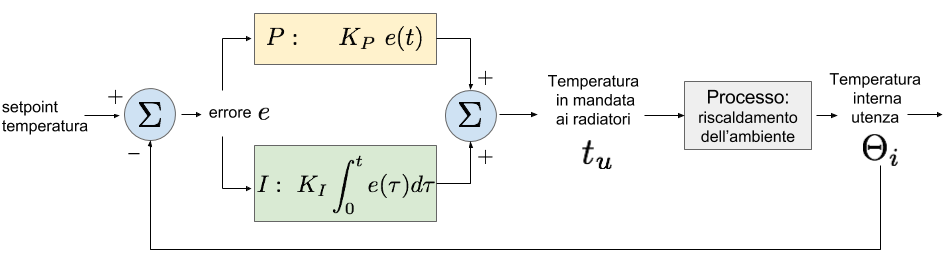
\includegraphics[width=0.95\textwidth]{figure/PI} 
\caption{Schema a blocchi di un controllore PI usato per la termoregolazione di un'utenza.}
\label{fig:PI}
\end{figure}
   
L'utente può in ogni caso impostare un valore di temperatura molto elevato nel termostato. Per aiutare l'utilizzatore dell'impianto di riscaldamento a fare ulteriore efficienza, la temperatura dell'acqua in mandata ai radiatori avrà un limite massimo sulla base della temperatura esterna e delle caratteristiche dell'edificio, secondo il concetto di termoregolazione climatica. 
Ovviamente questa temperatura limite dovrà garantire all'abitazione di potersi scaldare fino ad una temperatura di circa $20 ^{\circ}C$.

L'introduzione di questi limiti di saturazione sul controllore potrebbero introdurre effetti di windup.
Supponendo di applicare al sistema di riferimento un errore elevato, l'integratore inizierà ad accrescere il suo valore in uscita per via dell'errore non nullo. Quando il valore in uscita al controllore è tale da saturare il comando di attuazione, l'uscita dell'integratore continuerà a crescere fino a quando l'errore non diventerà nullo.
Il termine integrale può raggiungere valori molto elevati: è quindi richiesto che l'errore presenti segno opposto per un lungo periodo prima che si esca dalla saturazione. 
Questo fenomeno fa sì che il sistema dopo aver raggiunto la condizione di errore nullo, si allontani in direzione opposta, creando un effetto di sovraelongazione dalle caratteristiche non lineari. Una possibilità per ovviare a tale fenomeno consiste nel sospendere l'integrazione dell'errore quando il sistema è in saturazione.\\

% soluzione utilizzata o NON utilizzata (spiegare perchè)

La soluzione che utilizza una regolazione climatica PI per regolare il calore fornito ai radiatori, elimina le oscillazioni della temperatura interna dell'abitazione e richiede in ogni momento sempre la minima quantità di calore necessario per il comfort richiesto. Le temperature di ritorno dell'acqua alla centrale di scambio, saranno tanto più basse quanto minore è il carico termico richiesto. 

In Figura \ref{fig:reg_PID} è mostrato l'andamento delle temperature e portate di una sotto-centrale con regolazione PI.

\begin{figure}[!ht]
\centering
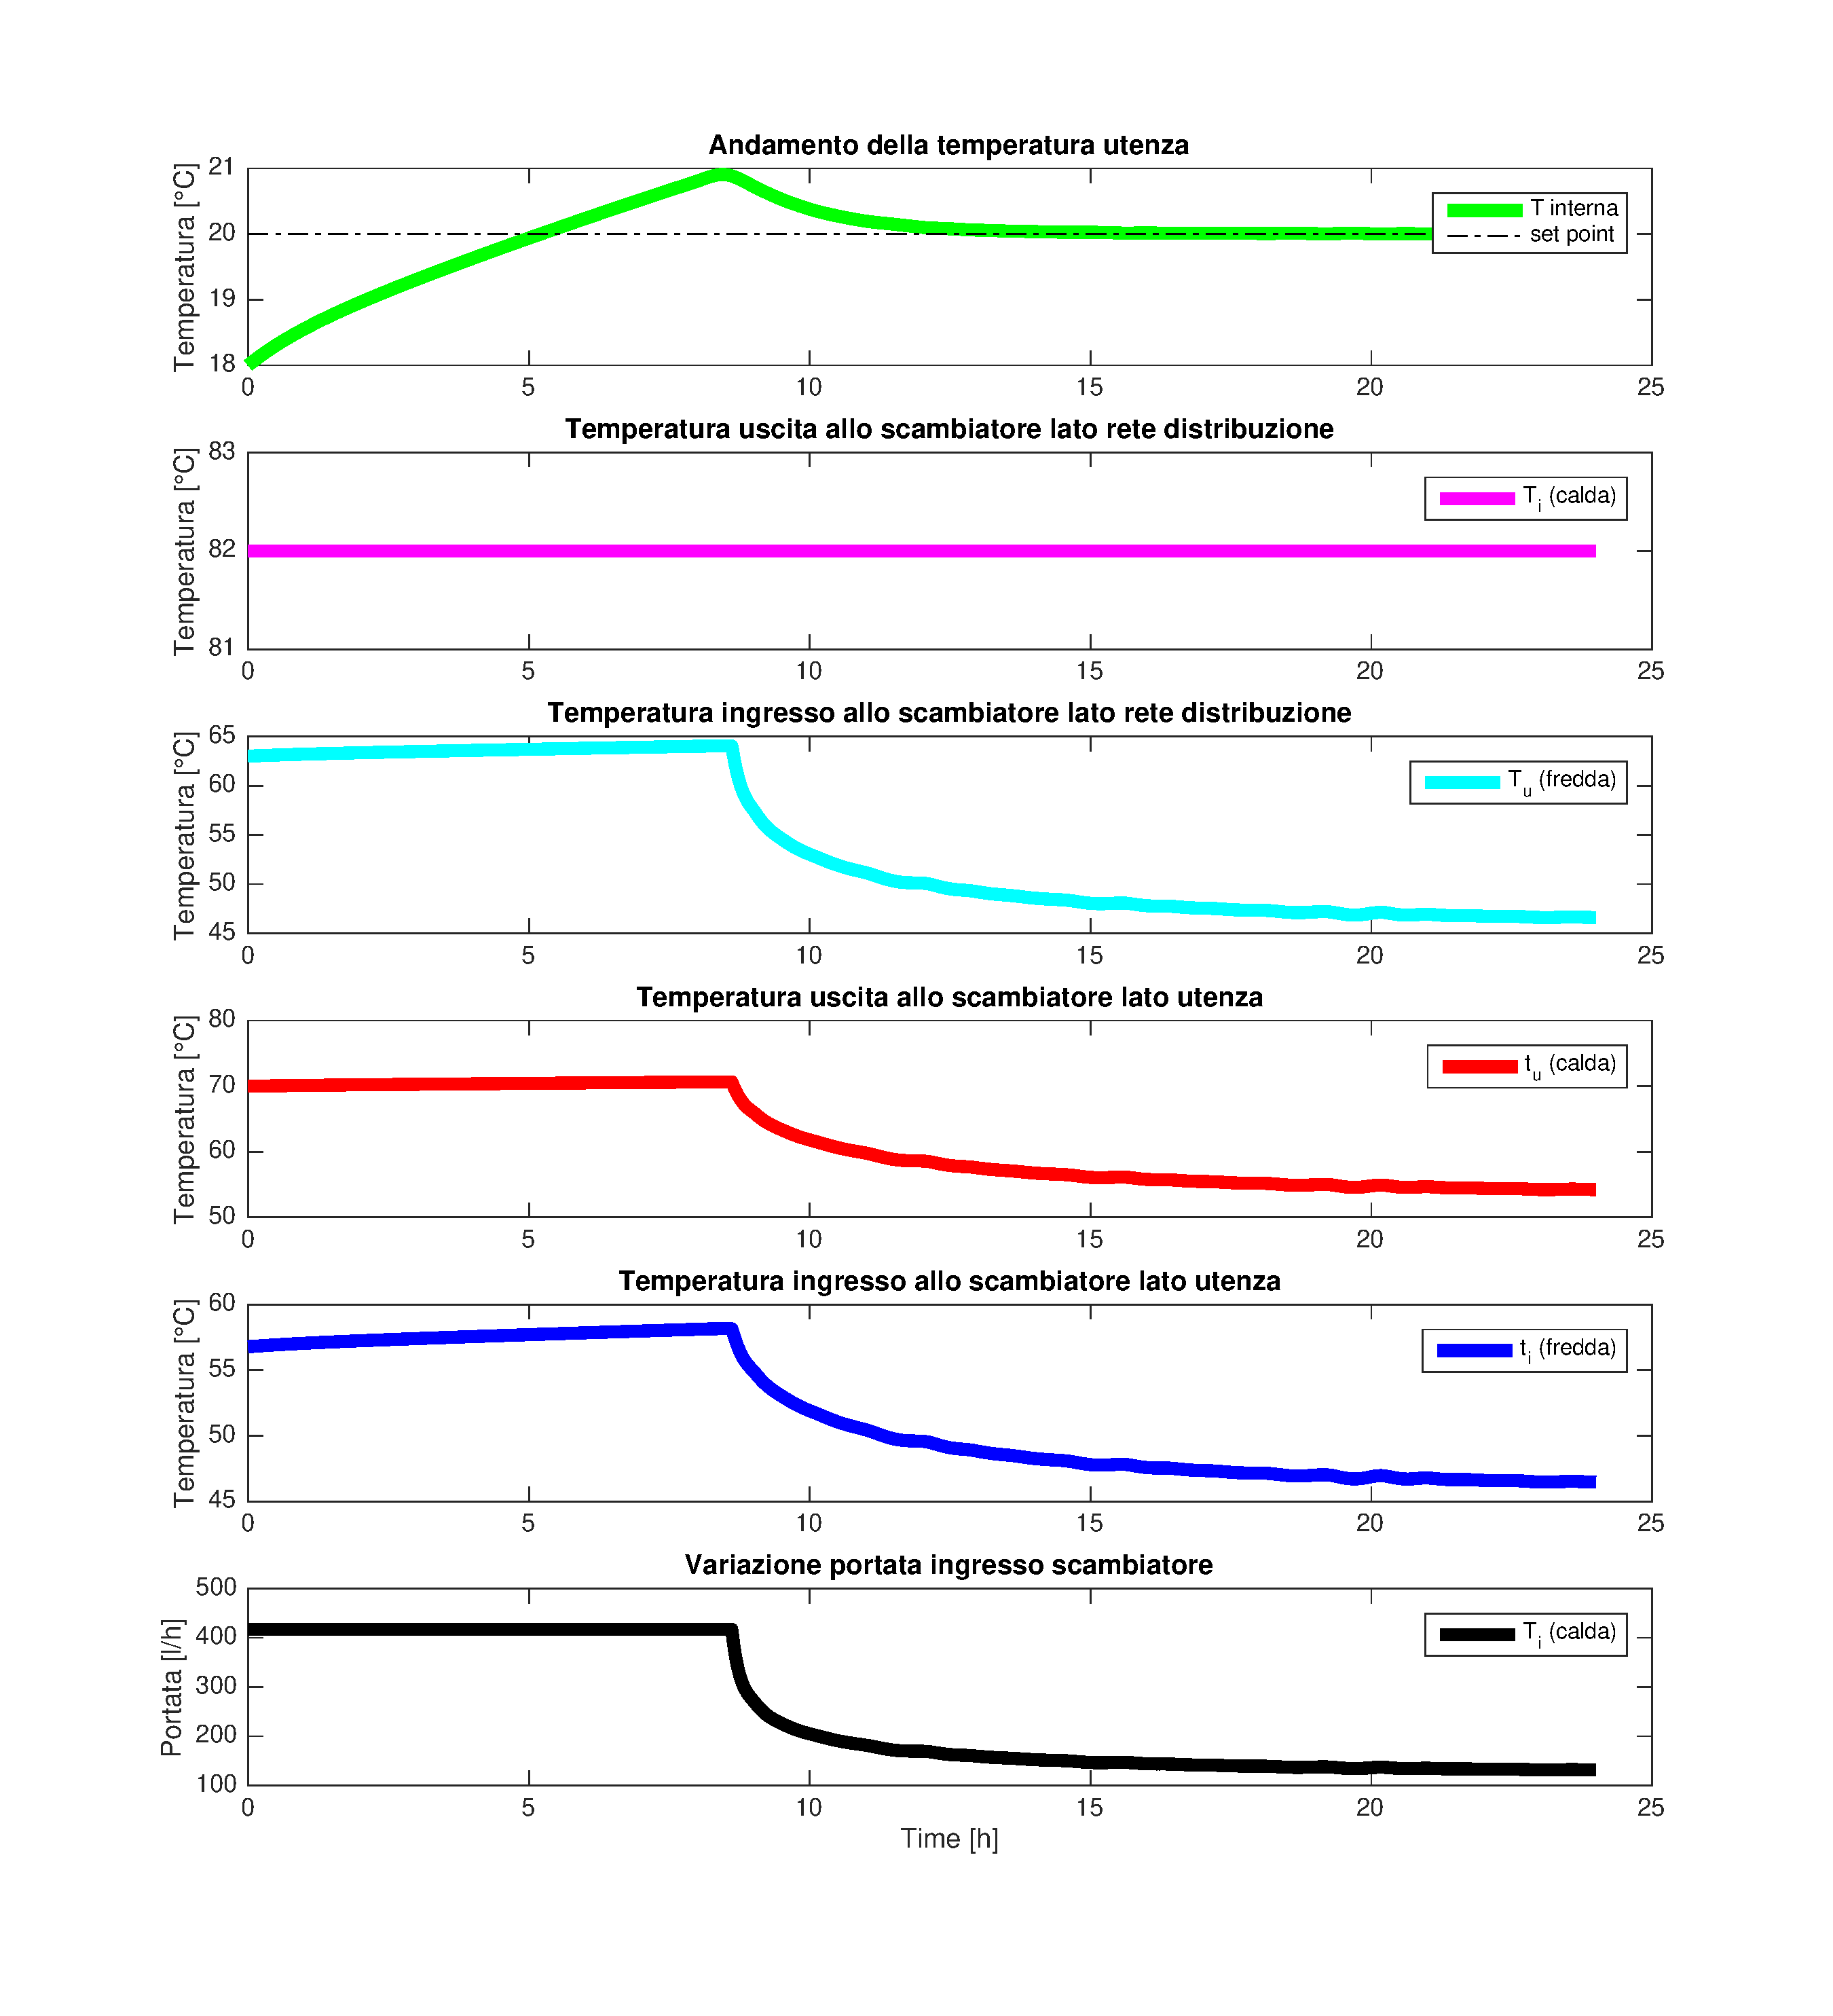
\includegraphics[width=\textwidth]{figure/reg_PID} 
\caption{Andamento della temperatura interna $\Theta_i$, delle temperature $T_i, T_u, t_u, t_i$ dello scambiatore e la portata per una sotto-centrale con regolazione climatica evoluta PI.}
\label{fig:reg_PID}
\end{figure}

La pompa di circolazione dell'utenza può rimanere sempre accesa in quanto è la centralina a determinare il giusto grado di laminazione della valvola per avere in casa la temperatura desiderata. 
 Una volta raggiunta la temperatura di comfort, questa regolazione è quella che spreca meno energia termica utilizzando esattamente il calore necessario a mantenere la temperatura interna costante. È la regolazione che richiede il minor flusso di acqua e fa tornare in centrale l'acqua alla più bassa temperatura possibile.  Inoltre, si evitano picchi di richiesta di calore dovuti all'accensione e allo spegnimento del riscaldamento che si hanno con i termostati comuni. 


\subsection{Variazione della velocità delle pompe di circolazione interne all'utenza}

%Potenze scambiate e temperature al variare delle por- tate

Le pompe di circolazione di acqua calda all'interno dell'abitazione lavorano a giri fissi ed i costi di energia elettrica per il loro funzionamento sono a carico dell'utilizzatore. Dal momento che la potenza erogata dai radiatori dipende anche dalla portata è facile pensare di poter  regolare la velocità delle pompe delle utenze per fornire il calore necessario al proprio fabbisogno. Inoltre, questa regolazione aiuterebbe le utenze a ridurre i costi di energia elettrica dovuti alla pompa di circolazione di casa.

Per verificare se questa regolazione effettivamente può portare a dei benefici abbiamo effettuato una simulazione valutando  l’andamento delle temperature e della potenza termica scambiata al variare delle portate.

Impostando la portata sul primario $G_p$ costante e la portata sul circuito dell'utenza $G_u$ variabile otteniamo i seguenti risultati.
Maggiore è la portata sul secondario minore risulta la differenza di temperatura tra $t_u$ e $t_i$ e viceversa. Il risultato più significativo ci mostra che variando la portata sul secondario, variano le temperature di mandata e ritorno ma variano in
modo tale che la loro temperatura media rimanga costante come anche la temperatura di ritorno della rete di distribuzione $T_u$ (Figura \ref{fig:pompa_var_utenza}).

\begin{figure}[!ht]
\centering
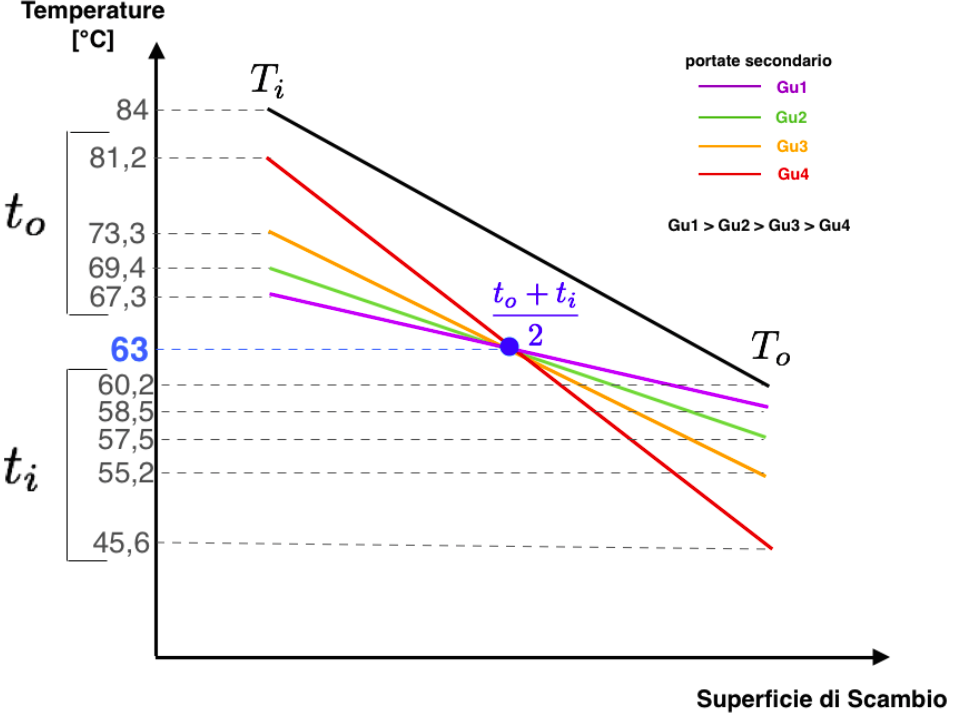
\includegraphics[width=0.85\textwidth]{figure/pompa_var_utenza} 
\caption{Rappresentazione schematica della variazione delle temperature di uno scambiatore al variare della portata sul circuito dell'utenza e portata del circuito principale costante}
\label{fig:pompa_var_utenza}
\end{figure}

In conclusione possiamo affermare che la potenza scambiata e la temperatura di ritorno $T_u$ dipende solamente dalla portata in mandata sul primario.
Questo ci conferma ulteriormente che la regolazione da implementare dovrà essere necessariamente inserita sulla portata del circuito primario in modo da limitare il ritorno di temperatura al minimo possibile ma tale da garantire la temperatura ambiente impostata nel termostato di casa.

\subsection{Regolazioni delle sotto-centrali di scambio a confronto}
Utilizzando come base di riferimento uno scambiatore senza regolazioni, si esamina come varia l'andamento della temperatura di ritorno alla centrale $T_u$ e la portata $G_p$ in arrivo allo scambiatore dal lato della rete di distribuzione  confrontando i seguenti tipi di regolazione: termoregolazione a punto fisso, termoregolazione climatica e regolazione climatica evoluta PI.

Utilizzando i dati ottenuti dalle simulazioni precedenti, in Figura \ref{fig:To_confronto}  si mostra l'andamento della  temperatura $T_u$ dei vari tipi di regolazione.

\begin{figure}[!ht]
\centering
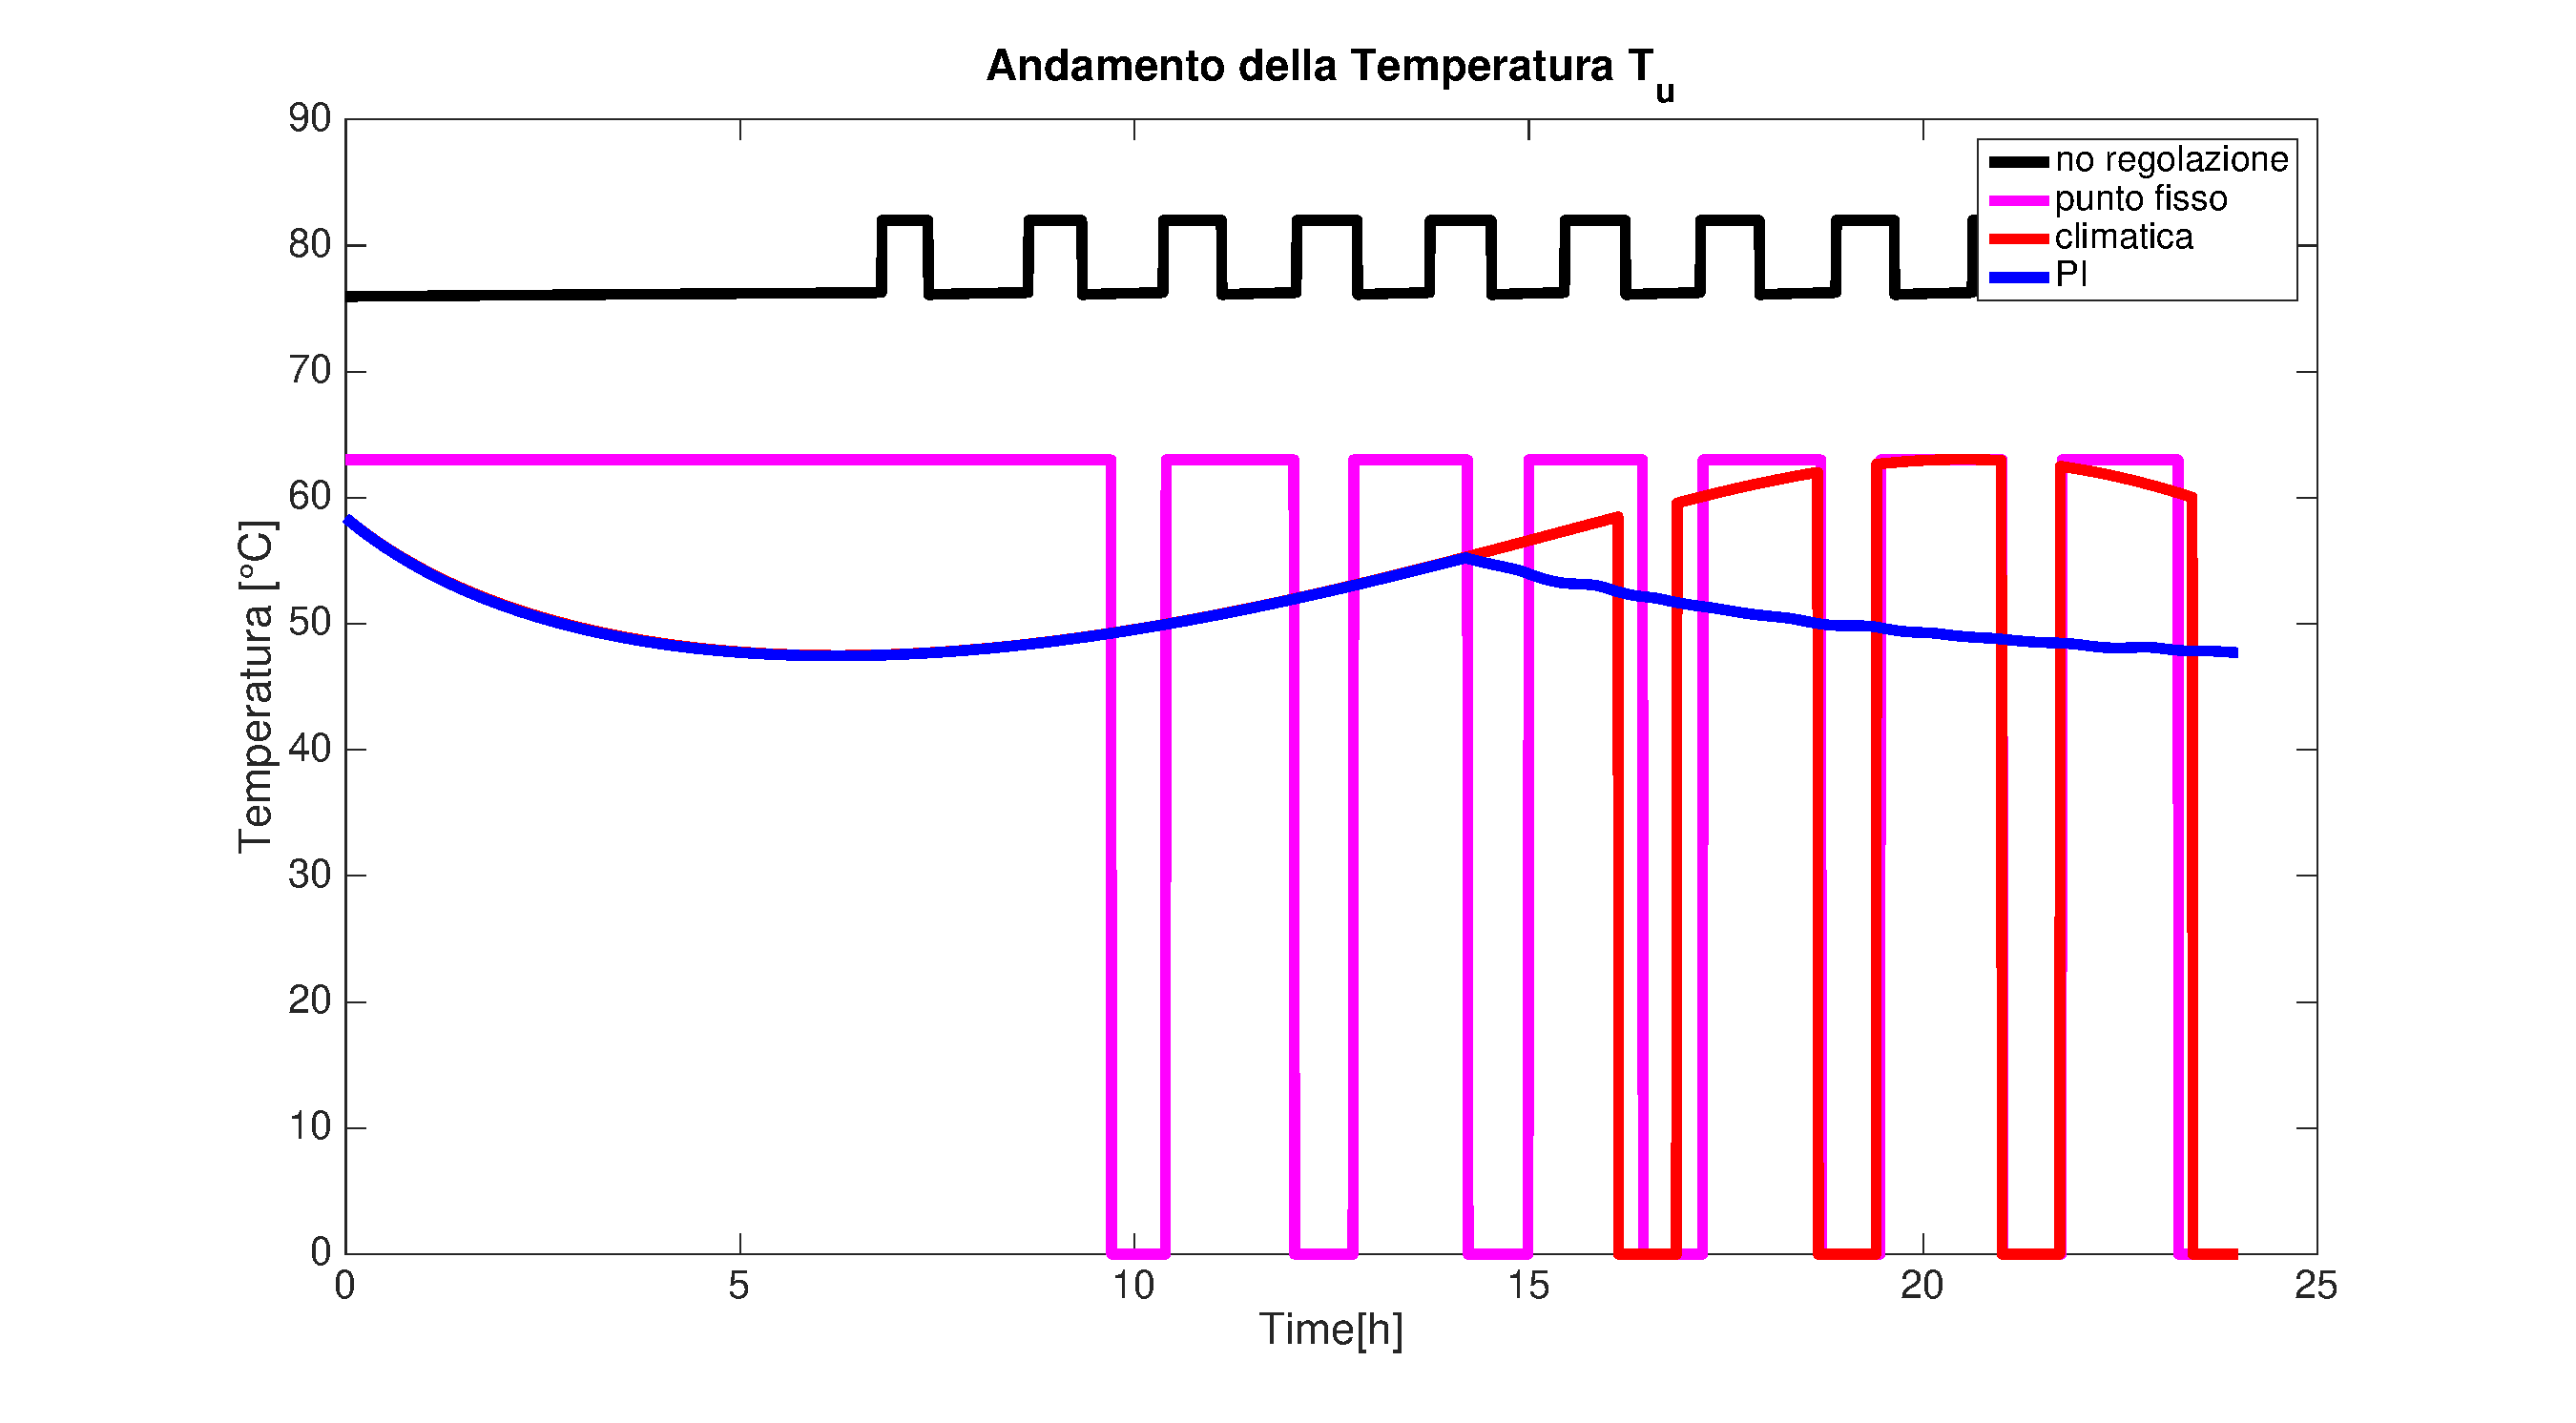
\includegraphics[width=\textwidth]{figure/To_confronto} 
\caption{Confronto tra l'andamento temperatura di ritorno alla centrale $T_u$ con diversi metodi di regolazione durante una simulazione di 24 ore.}
\label{fig:To_confronto}
\end{figure}

In Figura \ref{fig:portate_confronto} invece è rappresentato il grafico della portata in ingresso $G_p$ in ingresso allo scambiatore d'utenza delle regolazioni studiate. 

\begin{figure}[!ht]
\centering
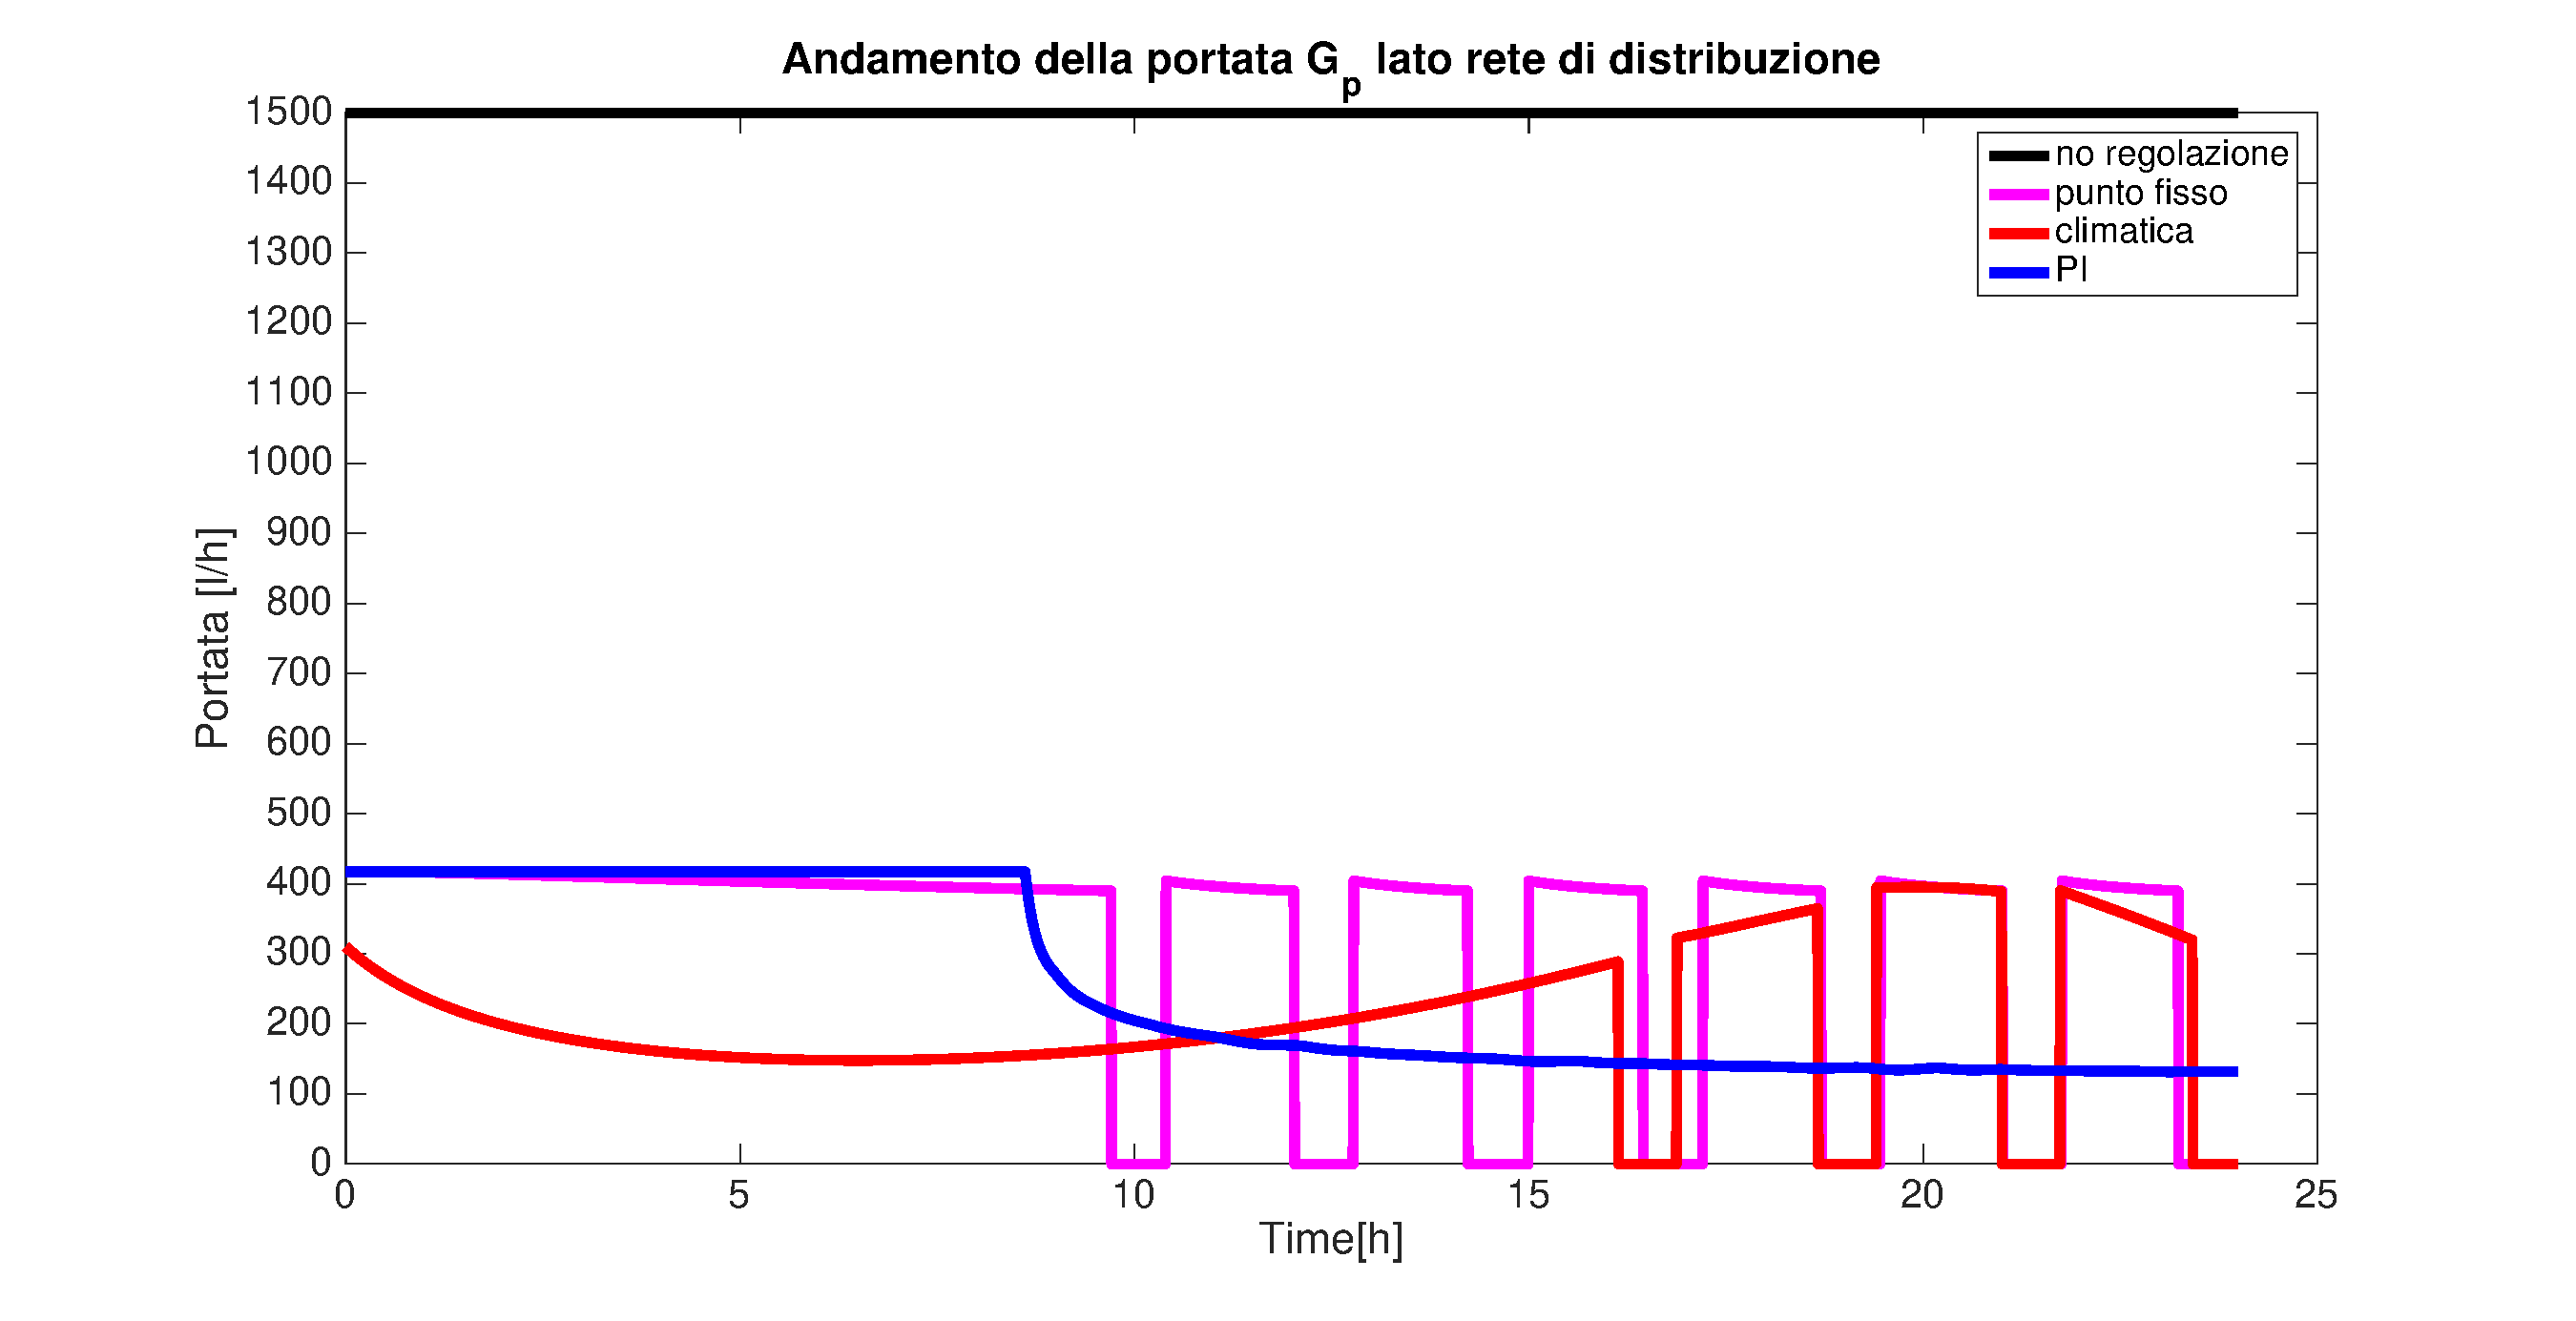
\includegraphics[width=\textwidth]{figure/portate_confronto} 
\caption{Confronto tra l'andamento delle portate con diversi metodi di regolazione durante una simulazione di 24 ore.}
\label{fig:portate_confronto}
\end{figure}

\textbf{Considerazioni sulle diverse regolazioni}
\begin{itemize}
\item Scambiatore senza regolazione: non essendoci alcun tipo di regolazione, quando il sistema di riscaldamento dell'utenza è spento, l'acqua circola comunque nello scambiatore senza però cedere colore perciò l'acqua ritornerà in centrale alla stessa temperatura di quella a cui è stata mandata. La stazione di pompaggio spreca energia senza che sia consumato calore. Questa configurazione è sicuramente la meno efficiente.
\item Termoregolazione a punto fisso: rispetto agli scambiatori senza regolazione si ha una riduzione della temperatura di ritorno $T_u$ e quando il riscaldamento è spento la valvola di laminazione si chiude in modo da non permettere il passaggio di acqua nello scambiatore. La temperatura di set point deve essere fissata ad una valore che permetta di scaldare la casa nelle condizioni peggiori possibili. Quindi, quando la temperatura esterna è maggiore di tale temperatura si fornirà surplus di  calore. Questo tipo di regolazione è economica ma sicuramente non la più efficiente.
\item Termoregolazione climatica: il funzionamento è molto simile alla termoregolazione a punto fisso, ma il set point di temperatura in mandata ai radiatori varia secondo una curva di compensazione in funzione della temperatura esterna. Minore è la temperatura esterna, maggiore sarà la temperatura di mandata $t_u$. Gli sprechi sono dunque ridotti al minimo e quando la temperatura esterna non è critica abbiamo delle temperature più basse rispetto alla regolazione a punto fisso e di conseguenza anche la portata necessaria sarà minore. Tra le regolazioni che prevedono l'utilizzo di un termostato è sicuramente la migliore in termini di efficienza.
\item Regolazione climatica evoluta PI: indubbiamente la migliore regolazione da installare in una sotto-centrale di utenza. Una volta che la temperatura ambiente si stabilizza al valore di comfort desiderato la  temperatura di ritorno $T_u$ sarà la minima raggiungibile. Utilizzando un controllore PI invece di un termostato (che produce un andamento oscillatorio tra due valori), si può mantenere sempre accesa la pompa di circolazione d'utenza limitando così i picchi di richiesta di calore sulla rete.


\end{itemize}



\section{Soluzioni per ridurre i consumi di energia di pompaggio}
La potenza assorbita da una pompa di circolazione è direttamente proporzionale alla portata ed alla prevalenza erogata come descritto dall'equazione (\ref{eq:pot}). Le due grandezze dovranno essere dunque ridotte allo stretto indispensabile per minimizzare i consumi di energia.
In prima istanza si potrebbe pensare di introdurre delle valvole di laminazione del flusso. Questa soluzione se da un lato riduce la portata dall'altro comporta un incremento della prevalenza in quanto aumenta la resistenza idraulica della rete.
Non necessariamente la sola introduzione di una valvola di regolazione riduce i consumi. Sarà dunque indispensabile poter cambiare la caratteristica della pompa in modo da ottenere  valori di portata che garantiscano a tutte le utenze allacciate all'impianto di teleriscaldamento di ottenere la giusta energia termica per il proprio fabbisogno, e di prevalenza tale da permettere il passaggio di acqua anche nelle utenze più svantaggiate.
Il tutto è reso possibile da degli inverter i quali permettono di modificare il numero di giri delle pompe di circolazione (e dunque far variare la caratteristica della pompa). I vantaggi sono riportati in seguito.

\subsection{Vantaggi di utilizzare pompe a velocità variabile}
Un numero crescente di aziende si sta accorgendo dell'importanza dell'efficienza energetica e dell'impatto che essa esercita sui costi e sui profitti dell'azienda.
In particolare, il prodotto che più immediatamente e in maniera consistente permette di conseguire dei risparmi energetici è l'inverter, soprattutto in applicazioni con movimentazione di fluidi, come ad esempio pompe centrifughe. Infatti, per tali applicazioni, è valida una legge fisica, chiamata "legge di affinità" descritta nell'equazione (\ref{eq:affinita}), la quale afferma che la potenza assorbita è proporzionale al cubo della velocità di rotazione del motore. Da tale condizione è facile capire come, dimezzando la velocità del motore, la potenza impiegata sarà di un ottavo della potenza a regime. 
Variando la velocità di rotazione della pompa, si modifica la sua curva caratteristica. Quando si raggiungono basse velocità di rotazione si verifica un calo sensibile del rendimento. Variando il numero di giri della pompa variano sensibilmente gli assorbimenti della potenza, come evidenziato anche dalle relazioni di proporzionalità. Gli effetti benefici della variazione di velocità sono facilmente comprensibili mettendo in relazione la tecnica di controllo “con valvola di laminazione” e con l’utilizzo di inverter. 

La valvola di laminazione effettua una riduzione della sezione della conduttura attraversata dal fluido, quindi in tale condizione se si desidera ridurre la portata della pompa centrifuga a portata inferiore, si sposta il punto di funzionamento, come risulta evidente dalla Figura \ref{fig:strozzatura}.

\begin{figure}[!ht]
\centering
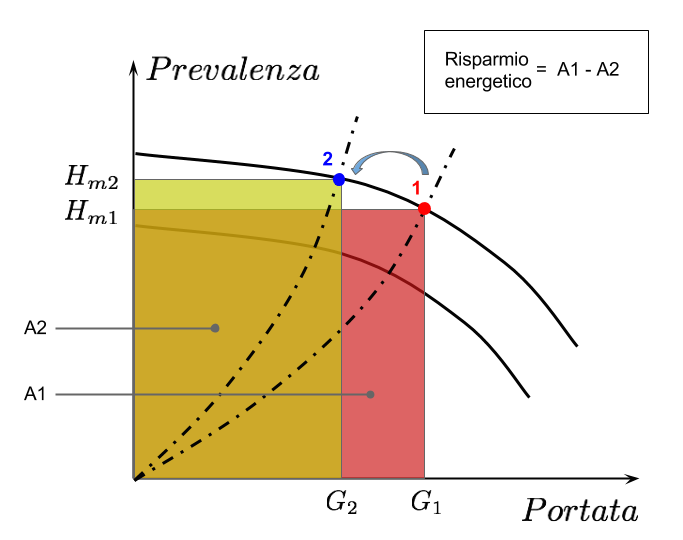
\includegraphics[width=0.75\textwidth]{figure/strozzatura} 
\caption{Rappresentazione dell'energia salvata riducendo la portata con valvola di laminazione.}
\label{fig:strozzatura}
\end{figure}

Il punto di funzionamento della pompa si sposta da $1$ a $2$, imponendo di fatto un maggiore valore di prevalenza dell'impianto. Utilizzando un inverter si riduce il numero di giri della pompa, quindi ci si sposta lungo la curva dell'impianto e non della pompa come è possibile vedere in Figura \ref{fig:var_velocita}. 

\begin{figure}[!ht]
\centering
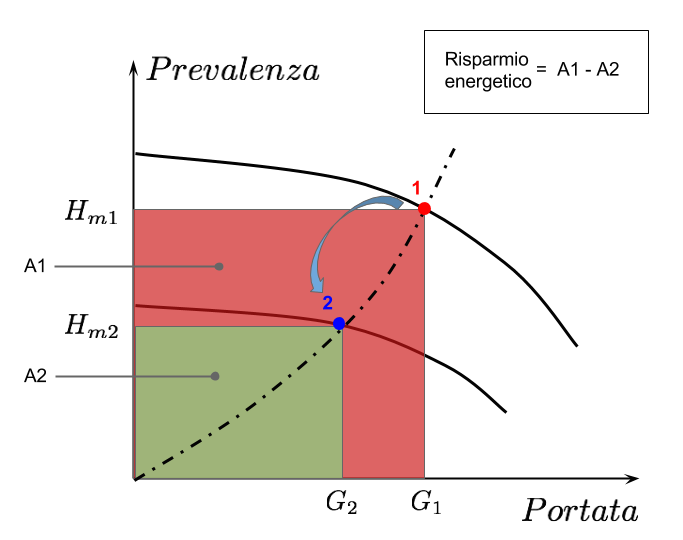
\includegraphics[width=0.75\textwidth]{figure/var_velocita} 
\caption{Rappresentazione dell'energia salvata riducendo la portata variando la velocità delle pompe.}
\label{fig:var_velocita}
\end{figure}

Dal punto di vista energetico la differenza è sostanziale: l'energia consumata è proporzionale alla differenza tra le due aree $A2$ e $A1$. Con la valvola di strozzatura il vantaggio è minimo, mentre nel secondo caso, grazie all'impiego di un inverter, l'incremento di efficienza energetica è decisamente più importante.


\section{Caratteristiche dell'impianto di Sant'Ippolito}
Il sistema analizzato in simulazione è la rete di teleriscaldamento chiamata S. Ippolito. \`E costituito da una centrale di scambio con scambiatore di calore vapore - acqua. La temperatura dell'acqua in mandata alla rete di distribuzione è regolata da una valvola di laminazione che regola il flusso di vapore in ingresso allo scambiatore. La temperatura desiderata di mandata è decisa arbitrariamente in base alla stagione. Nella centrale di scambio è presente una stazione di pompaggio con pompe a velocità variabile.
Le utenze allacciate ala rete dispongono di un sistema che regola il flusso in ingresso ai radiatori così da mantenere fissa la temperatura in mandata ai radiatori dell'abitazione. Questo tipo di regolazione aiuta ad abbattere la temperatura di ritorno rispetto a dei normali  scambiatori senza regolazioni di portata. La riduzione della temperatura di ritorno dovrebbe aiutare a limitare i consumi di energia di pompaggio, ma un sistema di regolazioni non adeguato rende il tutto vano. Le pompe sono controllate nel seguente modo. Si vuole mantenere la temperatura dell'acqua di ritorno alla centrale di scambio ad un certo valore di temperatura prestabilito. Dal momento che è possibile regolare la velocità delle pompe, questa regolazione   risulterebbe efficiente nel caso le utenze avessero una configurazione con valvole a tre vie come nel paragrafo \ref{subsec:3vie}. Nella situazione attuale, invece, quando le utenze richiedono poco calore, le valvole di laminazione si chiudono quasi totalmente facendo passare solo una piccola quantità di acqua nello scambiatore di utenza. L'acqua in circolo a causa della portata ridotta cederà gran parte del suo calore e l'abbattimento di temperatura sarà elevato. La situazione che si può verificare, è quella di avere l'acqua di ritorno a temperatura minore di quella impostata come set point cosicché i sensori ordineranno alle pompe di aumentare la velocità per incrementare la portata  nel circuito ed innalzare la temperatura dell'acqua. Ciò che si verifica è avere le pompe che lavorano quasi sempre al massimo dei giri sopratutto nei periodi con bassa richiesta di calore da parte delle utenze.

In seguito verranno descritte tutte le caratteristiche della rete e i parametri utilizzati per la simulazione

\subsection{Dati della rete di distribuzione}
La rete che andremo ad analizzare è descritta nella Tabella \ref{tab:rete_ippolito}. La conduttura primaria ha una lunghezza totale di 1848 $m$ a doppio tubo. Le tubazioni presenti sono pre-isolate con schiuma poliuretanica ed hanno diametri variabili. In Tabella \ref{tab:condotte} sono elencate e descritte le varie tipologie di tubazioni utilizzate nella rete.


\begin{table}[!ht]
\centering
\resizebox{\columnwidth}{!}{%
\begin{tabular}{|c|c|c|c|c|c|c|}
\hline
\multicolumn{7}{|c|}{Rete di distribuzione S. Ippolito}                                                                                                                                                       \\ \hline
\multicolumn{1}{|c|}{\multirow{2}{*}{Utenze}} & \multicolumn{2}{c|}{Condotta Primaria}                         & \multicolumn{2}{l|}{Condotta intermedia}          & \multicolumn{2}{c|}{Condotta secondaria} \\ \cline{2-7} 
\multicolumn{1}{|c|}{}                        & Tipo                  & \multicolumn{1}{l|}{Lunghezza {[}m{]}} & \multicolumn{1}{l|}{Tipo} & Lunghezza {[}m{]}     & Tipo         & Lunghezza {[}m{]}         \\ \hline
1                                             & \multirow{2}{*}{DN65} & \multirow{2}{*}{235,6}                 & \multirow{2}{*}{DN32}     & \multirow{2}{*}{12,7} & d.28         & 24,5                      \\ \cline{1-1} \cline{6-7} 
2                                             &                       &                                        &                           &                       & d.28         & 3,5                       \\ \hline
3                                             & DN65                  & 25,8                                   & -                         & -                     & d.28         & 57,6                      \\ \hline
4                                             & DN65                  & 20                                     & -                         & -                     & d.28         & 12,4                      \\ \hline
5                                             & DN65                  & 111                                    & -                         & -                     & d.28         & 33,7                      \\ \hline
6                                             & DN65                  & 1082                                   & -                         & -                     & d.28         & 36                        \\ \hline
7                                             & DN65                  & 65                                     & -                         & -                     & d.28         & 16,5                      \\ \hline
8                                             & \multirow{2}{*}{DN50} & \multirow{2}{*}{168}                   & \multirow{2}{*}{DN32}     & \multirow{2}{*}{70}   & d.28         & 34,5                      \\ \cline{1-1} \cline{6-7} 
9                                             &                       &                                        &                           &                       & d.28         & 40                        \\ \hline
10                                            & DN50                  & 109,8                                  & -                         & -                     & d.28         & 7,3                       \\ \hline
11                                            & DN50                  & 30,3                                   & -                         & -                     & DN40         & 341,2                     \\ \hline
\end{tabular}}
\caption{Descrizione della struttura della rete di distribuzione dell'impianto di S. Ippolito.}
\label{tab:rete_ippolito}
\end{table}


\begin{table}[!ht]
\centering
\begin{tabular}{|c|c|c|c|}
\hline
\multicolumn{4}{|c|}{Tipologie di condotte nella rete di distribuzione}                                                                                                                                                   \\ \hline
Nome & \begin{tabular}[c]{@{}c@{}}Diametro\\ interno {[}mm{]}\end{tabular} & \begin{tabular}[c]{@{}c@{}}Diametro \\ esterno {[}mm{]}\end{tabular} & \begin{tabular}[c]{@{}c@{}}Spessore \\ isolante {[}cm{]}\end{tabular} \\ \hline
DN65 & 70,3                                                                & 73,2                                                                 & 2,895                                                                 \\ \hline
DN50 & 54,5                                                                & 57,4                                                                 & 2,935                                                                 \\ \hline
DN40 & 43,1                                                                & 45,7                                                                 & 2,785                                                                 \\ \hline
DN32 & 37,2                                                                & 39,8                                                                 & 3,1                                                                   \\ \hline
d.28 & 24,2                                                                & 28                                                                   & -                                                                     \\ \hline
\end{tabular}
\caption{Elenco delle condotte usate nella rete di S. Ippolito e caratteristiche.}
\label{tab:condotte}
\end{table}

\subsection{Pompa di circolazione}

Per la pompa di circolazione dell'acqua nella rete di distribuzione abbiamo fatto riferimento a quella già presente nell'impianto. Si tratta di una ''\textsc{grundfos}'' modello ''\textsc{TP40 - 470/2}'' con portata e prevalenza nominale rispettivamente di 29,2 $l/h$ e 32,5 $m$ a 2920 $min^{-1}$.
Le curva caratteristica della pompa e la sua curva di rendimento sono mostrate in Figura \ref{fig:curve_pompa}.

\begin{figure}[!ht]
\centering
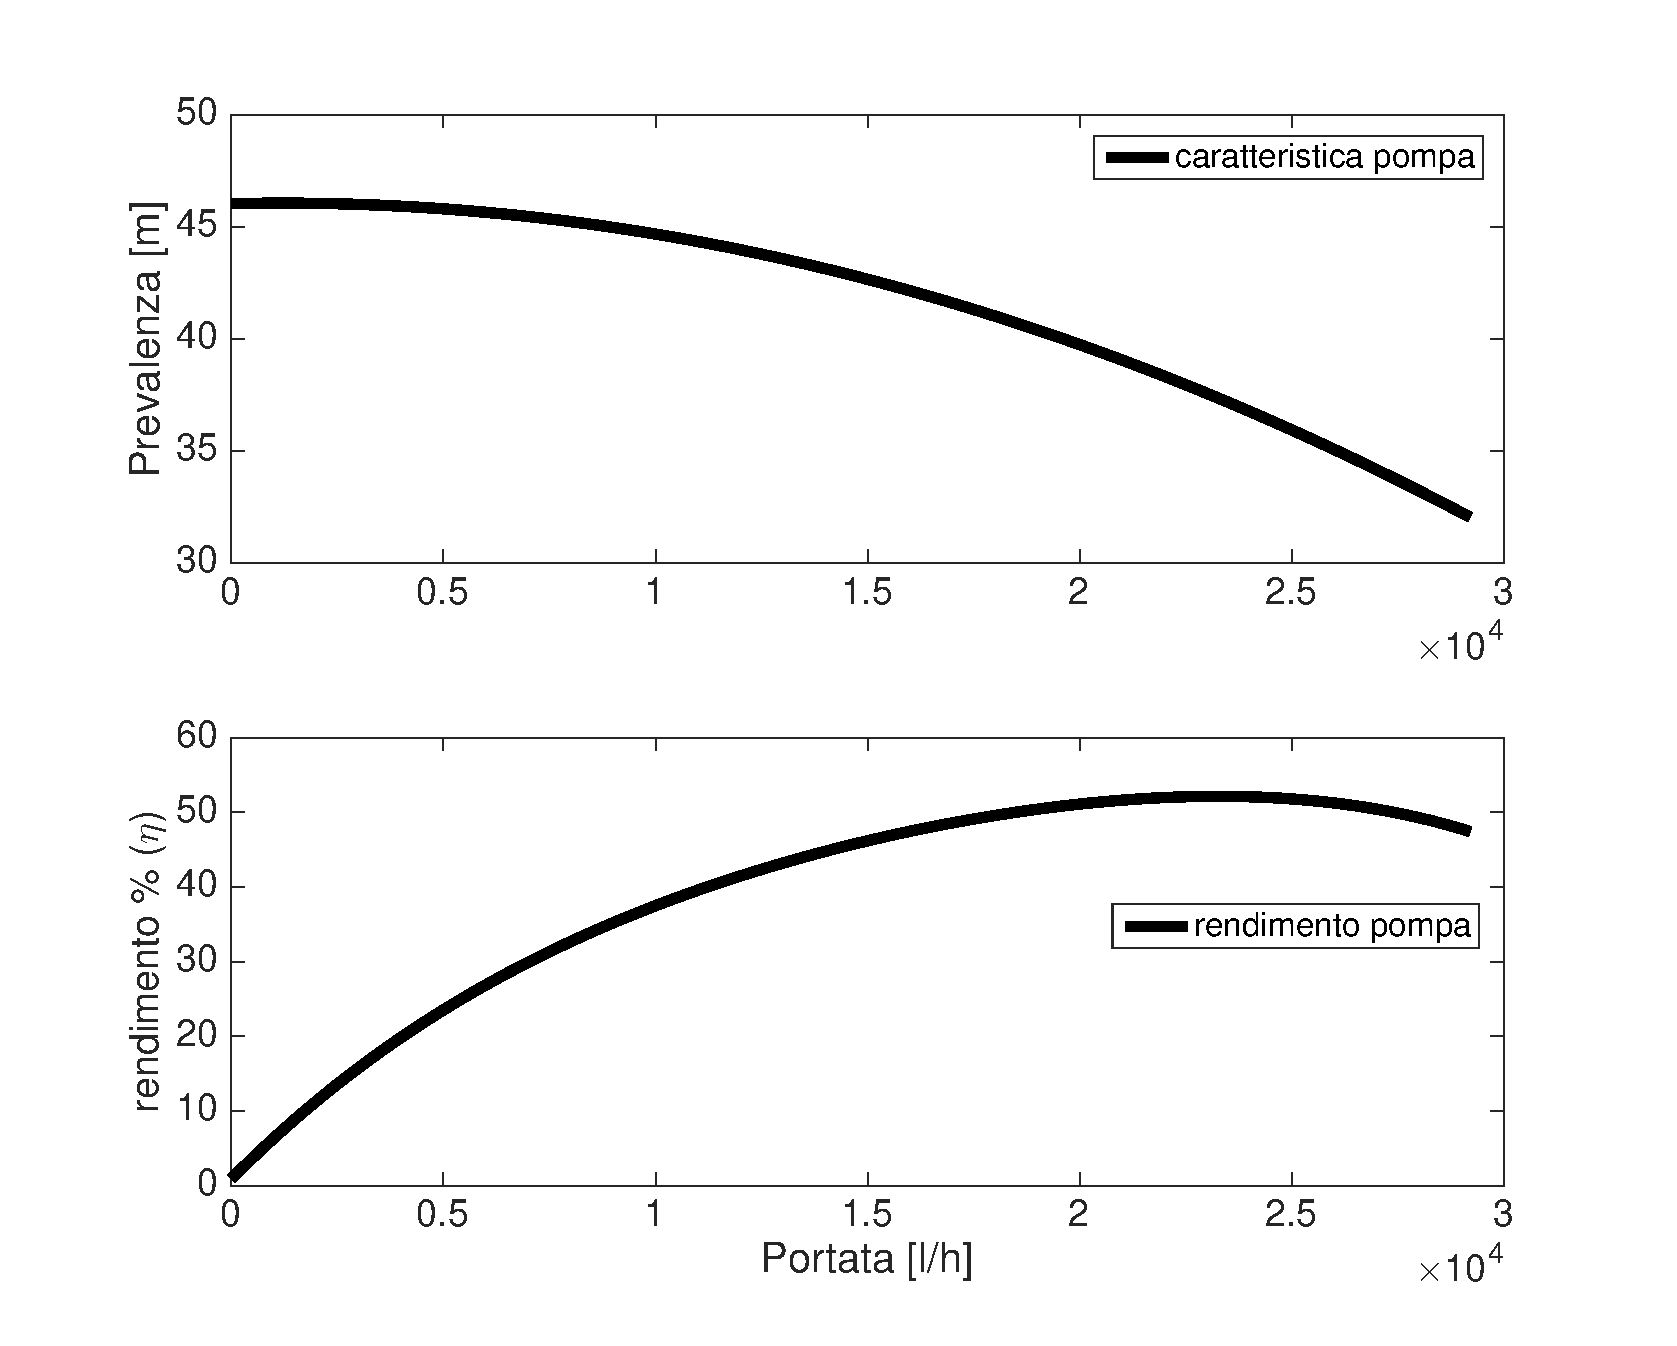
\includegraphics[width=\textwidth]{figure/curve_pompa} 
\caption{Curve della pompa utilizzata per la circolazione dell'acqua nella rete di distribuzione di S. Ippolito. }
\label{fig:curve_pompa}
\end{figure}

\subsection{Dati delle utenze allacciate alla rete}
In Tabella \ref{tab:par_utenze} sono mostrati tutti i parametri delle utenze utilizzati in simulazione. Un parametro comune a tutte le utenze è l'esponente $n$ dei radiatori uguale ad 1,32.
La descrizione dettagliata dei parametri che andremo a definire si trova nel capitolo 3. 

\begin{table}[!ht]
\centering
\resizebox{\columnwidth}{!}{%
\begin{tabular}{|c|c|c|c|c|c|c|c|c|c|}
\hline
& & & & & & & & & \\
\textbf{Utenza} & \multicolumn{1}{c|}{\textbf{V}} & \textbf{M$_a \cdot$ c$_a$ } & \textbf{M$_p \cdot$ c$_p$} & \textbf{R$_{ip}^{-1}$} & \textbf{R$_{pe}^{-1}$} & \textbf{R$_{f}^{-1}$} & \textbf{K$m$} & \textbf{$\alpha \cdot S$} & \textbf{G$_u$} \\ 
 &[$m^3$] &[$kcal/^{\circ}C$] &[$kcal/^{\circ}C$] & [$kcal/^{\circ}C$] &[$kcal/^{\circ}C$] &[$kcal/^{\circ}C$] &[$kcal/^{\circ}C$] & [$kcal/^{\circ}C$] & [$l/h$]\\ \hline
1               & 421                                      & 3490         & 167909       & 2654        & 172.6       & 135.7       & 72.23       & 2526        & 840         \\ \hline
2               & 475                                      & 3938         & 18609        & 2942        & 191.4       & 144.1       & 81.5        & 2850        & 950         \\ \hline
3               & 500                                      & 4145         & 19446        & 3073        & 200         & 147.9       & 85.8        & 3000        & 1000        \\ \hline
4               & 300                                      & 2487         & 12629        & 1996        & 129.9       & 114.5       & 51.5        & 900         & 600         \\ \hline
5               & 1200                                     & 9949         & 41985        & 6636        & 431.7       & 229         & 205.9       & 7200        & 2400        \\ \hline
6               & 776                                      & 6433         & 28494        & 4505        & 293         & 184.2       & 133.2       & 4656        & 1550        \\ \hline
7               & 600                                      & 4974         & 22759        & 3598        & 234         & 162         & 103         & 3600        & 1200        \\ \hline
8               & 680                                      & 5638         & 25379        & 4012        & 261         & 172.4       & 116.7       & 4080        & 1360        \\ \hline
9               & 1200                                     & 9949         & 41985        & 6636        & 431.7       & 229         & 205.9       & 7200        & 2400        \\ \hline
10              & 2100                                     & 17410        & 69830        & 11038       & 718         & 303         & 360.3       & 12600       & 4200        \\ \hline
11              & 2200                                     & 18239        & 72883        & 11520       & 749.4       & 310.2       & 377.5       & 13200       & 4400        \\ \hline
\end{tabular}}
\caption{Elenco dei parametri utilizzati in simulazione per ogni utenza.}
\label{tab:par_utenze}
\end{table}

\section{Simulazioni}
Nelle simulazioni che andremo ad effettuare, si vuole mostrare quale regolazione, ovvero quale sistema di limitazione della portata in ingresso allo scambiatore d'utenza, sia migliore al fine di ottenere i più bassi consumi di energia elettrica per il pompaggio dell'acqua nella rete di distribuzione. Verrà effettuata una simulazione per ogni tipo di regolazione esaminata nei paragrafi precedenti per un periodo di 24 ore. Inizialmente le utenze partiranno da una temperatura di 18 $^{\circ}C$ con pareti a 15 $^{\circ}C$ per arrivare ad una temperatura desiderata di 20 $^{\circ}C$. Inizialmente partiamo da una temperatura interna inferiore a quella di set-point per vedere come si comporta il sistema di fronte ad un picco di richiesta di energia termica. La temperatura esterna segue un andamento come quello della Figura \ref{fig:temp_est}.

Quando le utenze hanno regolazioni sul flusso di acqua in ingresso allo scambiatore possiamo cercare di ottimizzare i consumi di energia elettrica per il pompaggio utilizzando una pompa a giri variabili che si adatta in base ai valori di portata richiesti dalle abitazioni. Dobbiamo immaginare come se tutte le utenze comunicassero alla centrale termica la portata in ingresso allo scambiatore a loro necessaria in quel momento, di conseguenza la pompa dovrà essere in grado di adattarsi ad una certa velocità tale da garantire una portata uguale alla somma delle portate richieste e allo stesso tempo la potenza istantanea dovrà essere la minima possibile.\\

In seguito si analizzeranno in consumi delle pompe a velocità variabile e a velocità fissa per ogni tipo di regolazione sull'utenza applicate alla rete di Sant'Ippolito. 

\subsection{Simulazione rete senza regolazioni}
Il sistema di teleriscaldamento preso in esame già dispone di regolazioni di portata anche se il controllo sulla velocità della pompa è completamente sbagliato. Detto questo, come primo caso, prendiamo la nostra rete con sotto-stazioni d'utenza prive di regolatori di portata per vedere come si comporta l'impianto e quali a conclusioni possiamo arrivare. 

Dal momento che non sono presenti regolazioni a livello d'utenza è assolutamente inutile andare ad inserire ad esempio un inverter per controllare il numero di giri della pompa in base alla differenza di pressione tra mandata e ritorno misurata. Infatti, prevalenza e portata dipendono solamente da come è costruita la rete e non può variare nel tempo dato che non è presente nessun elemento di controllo che possa far variare i flussi d'acqua in ingresso agli scambiatori d'utenza.

Detto ciò in Figura \ref{fig:sim1_noreg} si può vedere quale sia il punto di funzionamento dell'impianto, ovvero il punto di intersezione tra la curva caratteristica della pompa e la curva caratteristica della rete di distribuzione.

\begin{figure}[!ht]
\centering
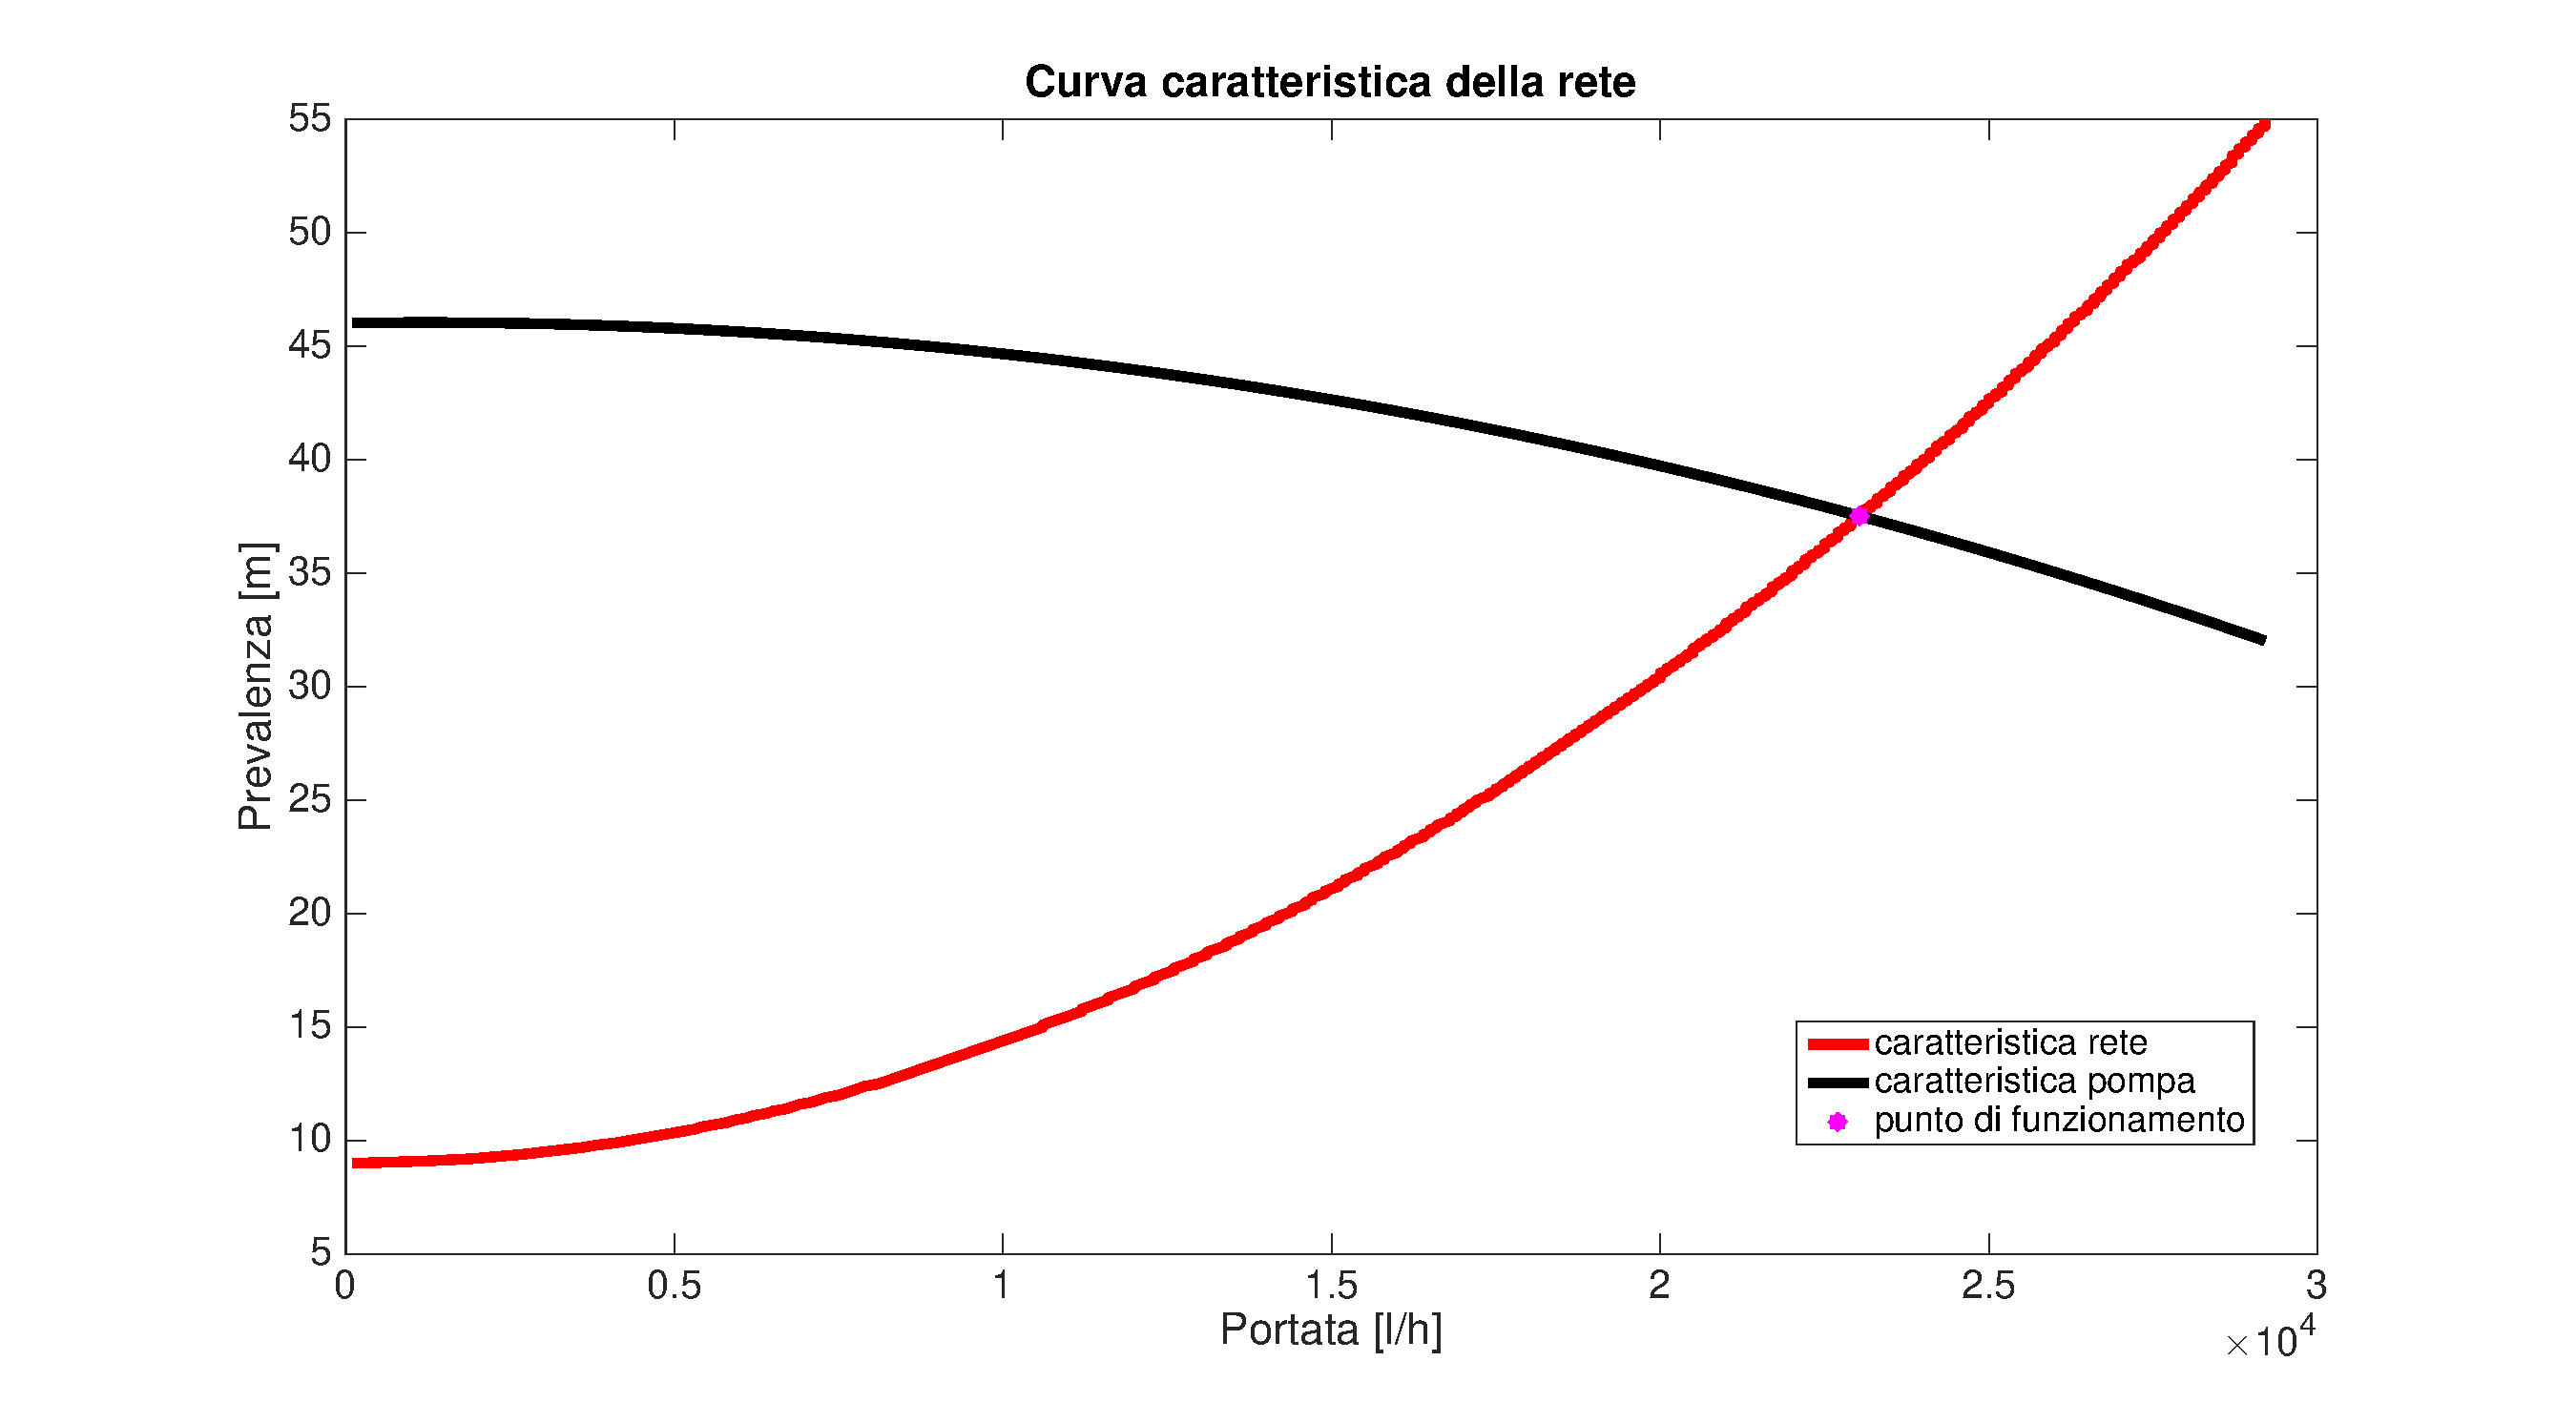
\includegraphics[width=\textwidth]{figure/sim1_noreg} 
\caption{Curva caratteristica della pompa e curva caratteristica della rete di distribuzione. L'intersezione delle due determina il punto di lavoro della pompa. }
\label{fig:sim1_noreg}
\end{figure}

Si nota che il punto di funzionamento ha:
\begin{itemize}
\item[-] Portata : 23040 $l/h$
\item[-] Prevalenza: 37,5 $m$
\item[-] Rendimento \% ($\eta$): 52,1%
\end{itemize}

La potenza istantanea della pompa sarà quindi di:
\begin{itemize}
\item[-] Potenza istantanea = 4,52 $kW$
\end{itemize}
Il consumo di energia elettrica della pompa nelle 24 ore di simulazione è:
\begin{itemize}
\item[-] Energia consumata = 108,43 $kWh$
\end{itemize}

Andando più nel dettaglio, in Figura \ref{fig:sim2_noreg}, si può vedere le portate in ingresso ad ogni utenza e le perdite di carico della rete. 

\begin{figure}[!ht]
\centering
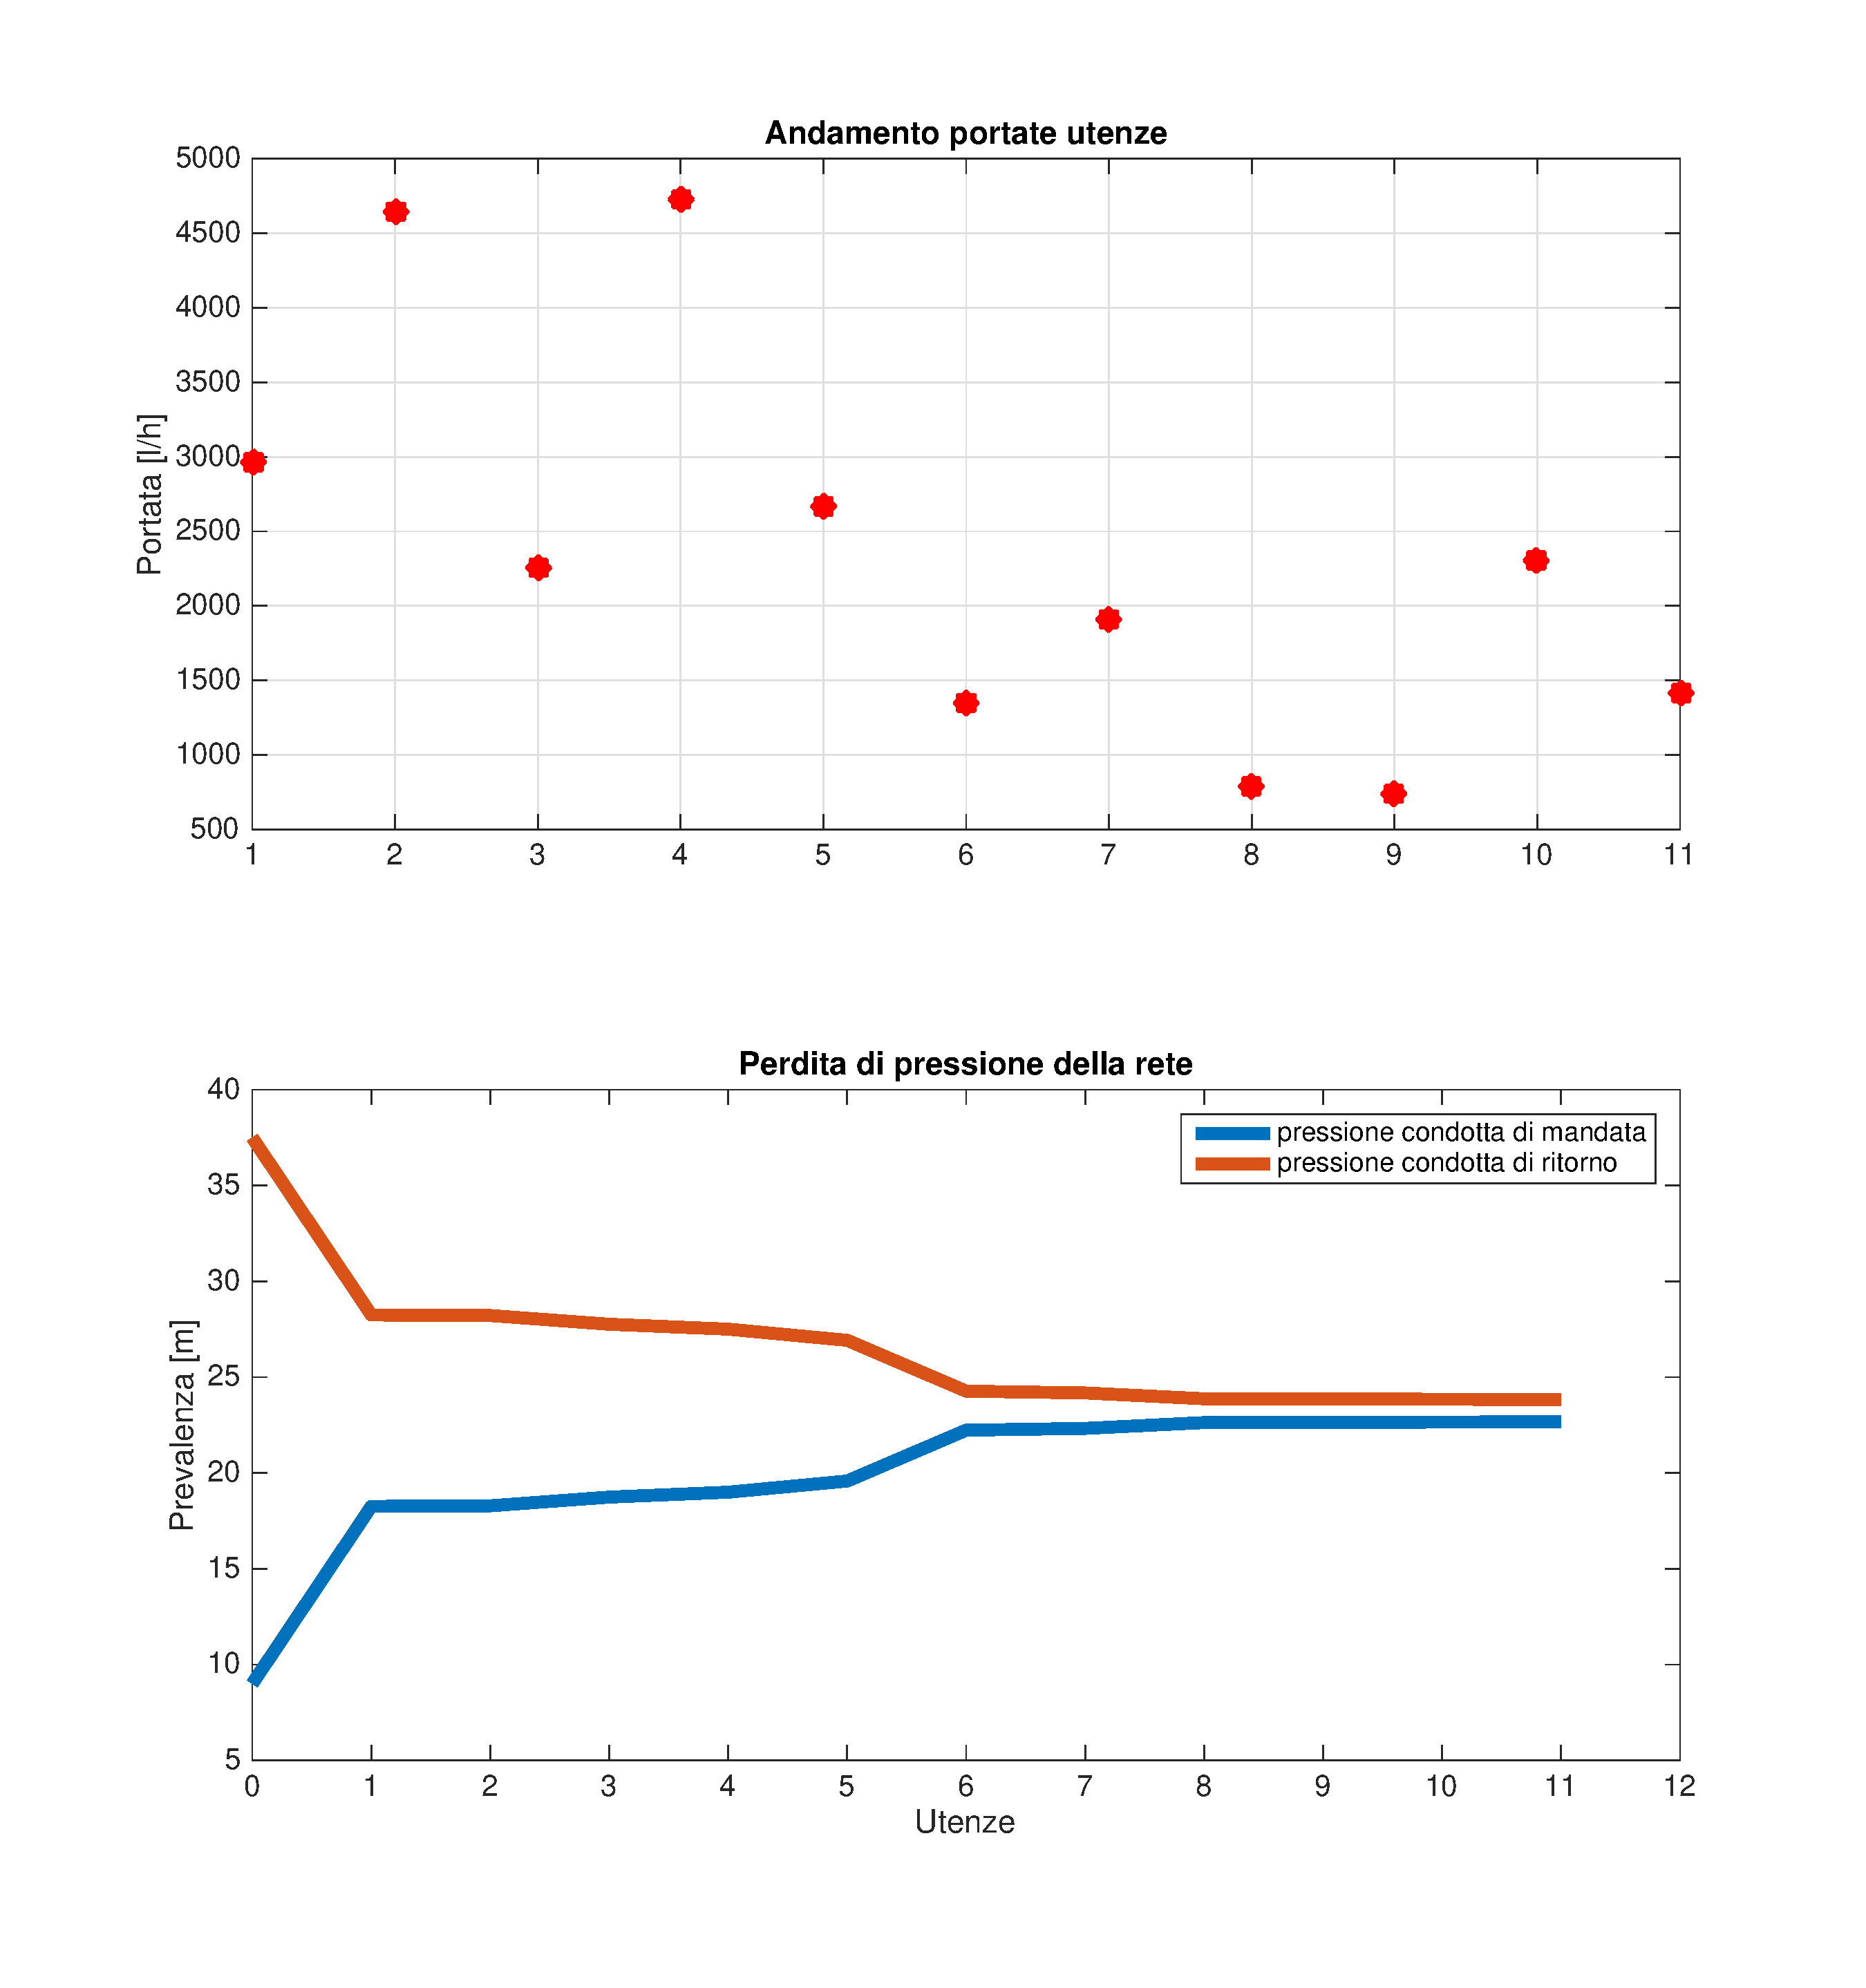
\includegraphics[width=\textwidth]{figure/sim2_noreg} 
\caption{Portate in ingresso agli scambiatori d'utenza e perdite di carico della rete. }
\label{fig:sim2_noreg}
\end{figure}

Si può notare come le prime utenze possano disporre di un flusso maggiore di acqua rispetto le ultime. Le abitazioni posizionate più vicine alla centrale termica avranno un costante surplus di energia mentre le più lontane rischiano di avere i radiatori freddi. Essendo per di più le ultime utenze quelle con volumetrie maggiori, la portata entrante nello scambiatore dovrebbe essere di gran lunga superiore a quella fornitagli in questo caso. 

Per funzionare correttamente uno scambiatore dovrebbe avere almeno una differenza di pressione tra ingresso e uscita di circa 5 $m$. Questo vincolo non è raggiunto dalle ultime sei utenze. 
Ciò evidenzia come l'utilizzo di scambiatori senza regolazioni per questo tipo di rete sia assolutamente controindicato.


\subsection{Simulazione della rete con termoregolazione a punto fisso sulle utenze}
Nella prossima simulazione andremo a verificare il comportamento della rete quando sono presenti termoregolazioni a punto fisso sulle utenze. 

La temperatura di set-point dell'acqua in ingresso ai radiatori è impostata a 70 $^{\circ}$C.

In Figura \ref{fig:sim_regmandata} è mostrato l'andamento della prevalenza, portata e potenze istantanee della pompa di circolazione.

\begin{figure}[!ht]
\centering
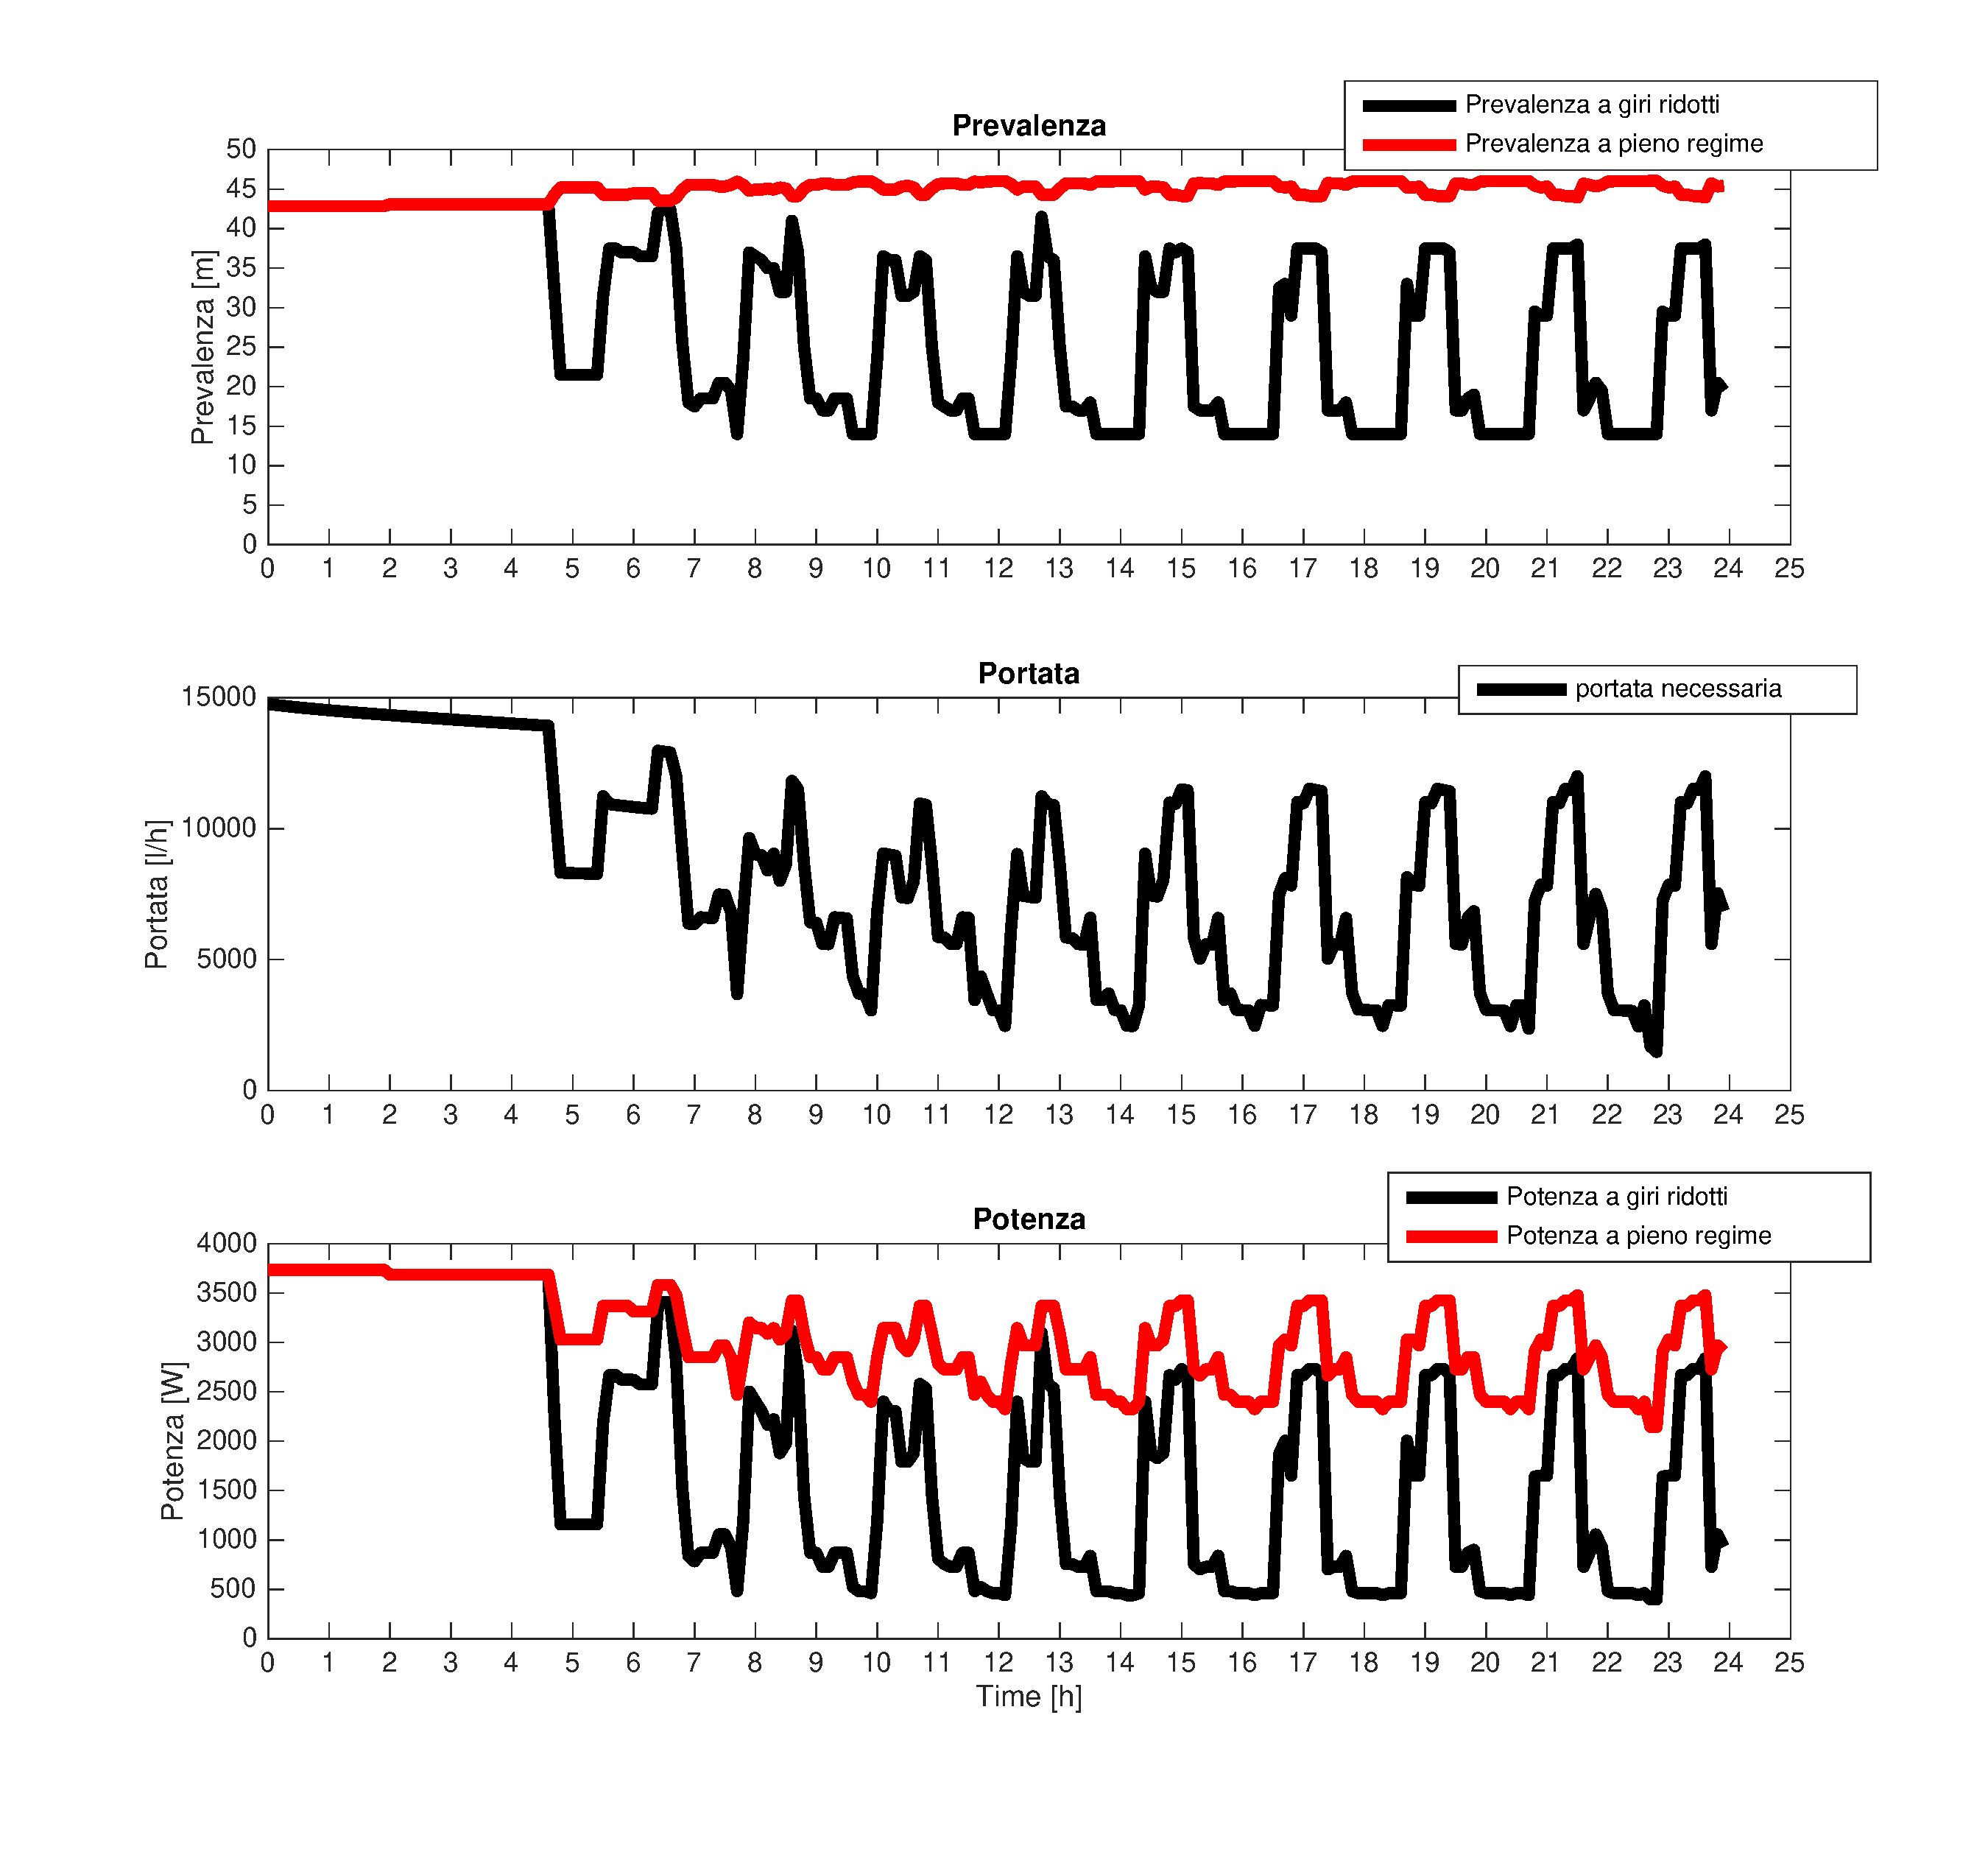
\includegraphics[width=\textwidth]{figure/sim_regmandata} 
\caption{Prevalenza, portata e potenza istantanea della pompa con termoregolazione a punto fisso sulle utenze. }
\label{fig:sim_regmandata}
\end{figure}

Il consumi della pompa risultano:
\begin{itemize}
\item[-] Consumo di energia elettrica con pompe a giri variabili: 44,19 $kWh$ 
\item[-] Consumo di energia elettrica con pompe a pieno regime: 73,08 $kWh$
\end{itemize}

\subsection{Simulazione della rete con termoregolazione climatica sulle utenze}
In seguito andremo a verificare il comportamento della rete quando sono presenti termoregolazioni climatiche sulle utenze. 

La curva di compensazione fa riferimento alla seguente retta:
\begin{equation}
y = -1,65 x + 68
\end{equation}
Al posto della $x$ dovremmo sostituire i valori della temperatura esterna misurati dalla sonda ed otterremo la temperatura di set-point $t_u$ in mandata ai radiatori  desiderata.

In Figura \ref{fig:sim_climatica} è mostrato l'andamento della prevalenza, portata e potenza istantanea della pompa di circolazione.

\begin{figure}[!ht]
\centering
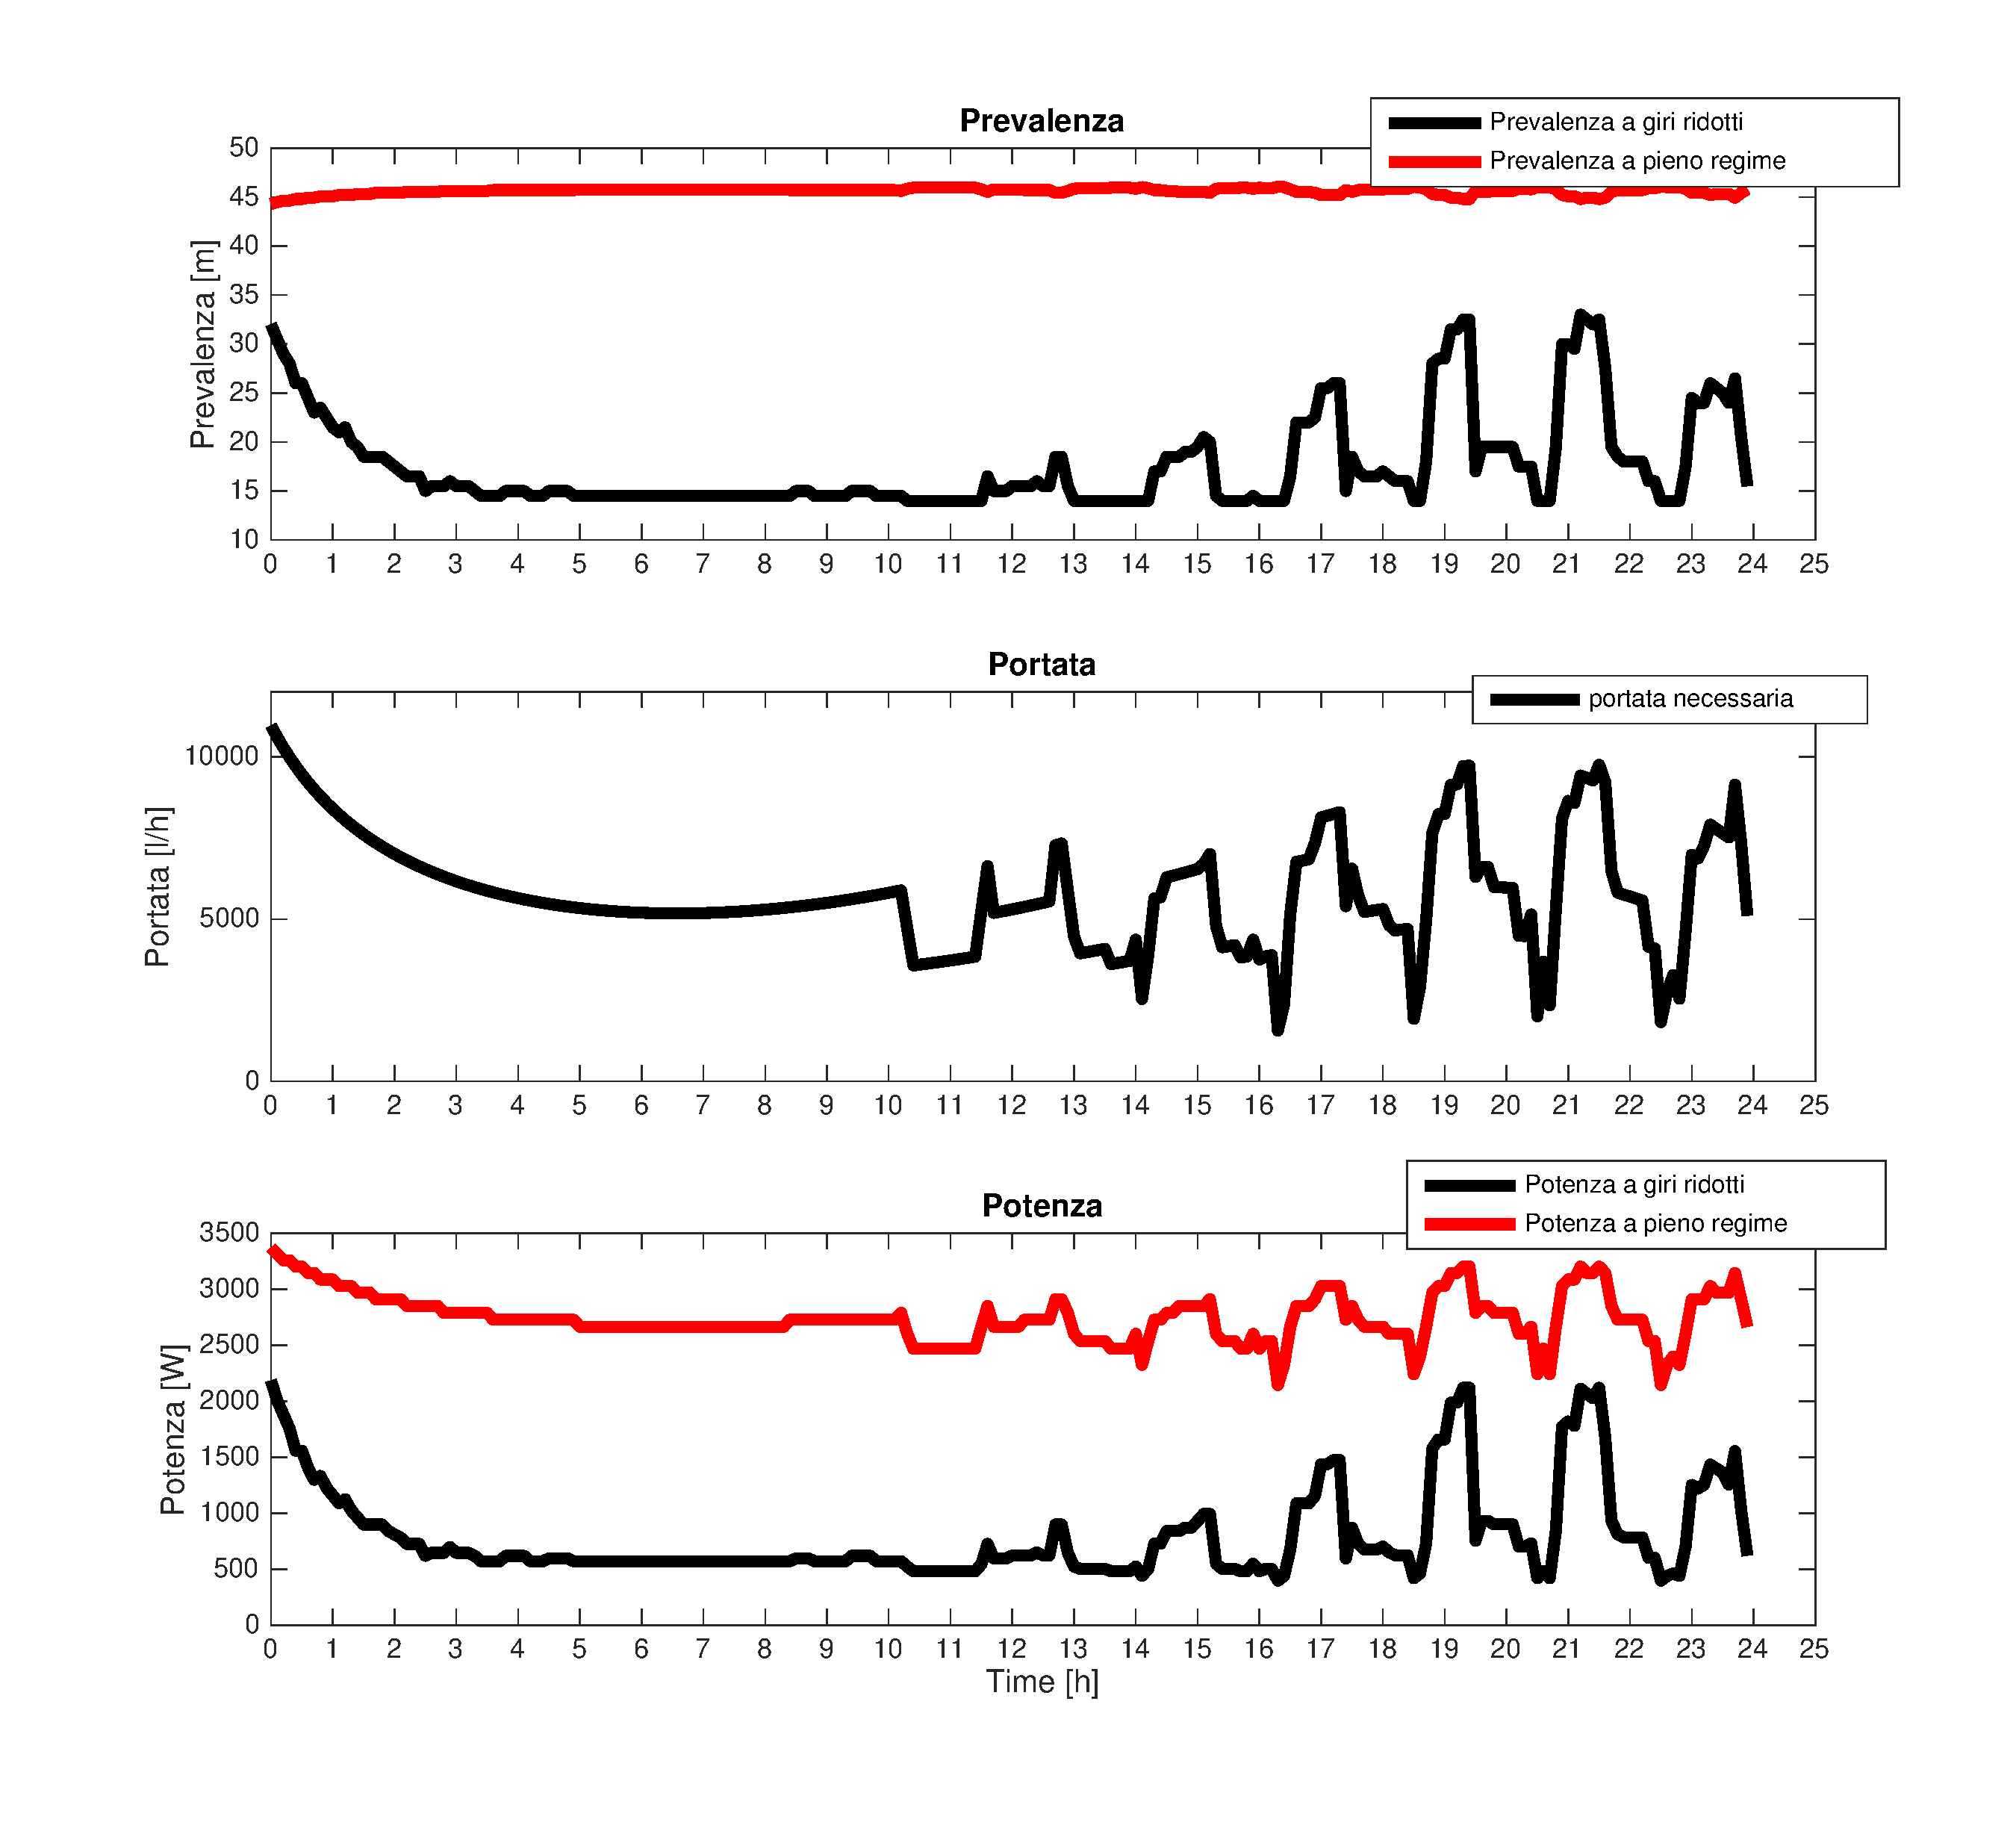
\includegraphics[width=\textwidth]{figure/sim_climatica} 
\caption{Prevalenza, portata e potenze istantanee della pompa con termoregolazione climatica sulle utenze.}
\label{fig:sim_climatica}
\end{figure}

Il consumi della pompa risultano:
\begin{itemize}
\item[-] Consumo di energia elettrica con pompe a giri variabili: 19,20 $kWh$ 
\item[-] Consumo di energia elettrica con pompe a pieno regime: 65,88 $kWh$
\end{itemize}

\subsection{Simulazione della rete con regolazione climatica evoluta PI sulle utenze}
Nella sezione si andrà a studiare il comportamento della rete quando sono presenti regolazioni climatiche evolute PI sulle utenze.  La curva di compensazione fa riferimento alla curva descritta nell' equazione (4.1).

In Figura \ref{fig:sim_PID} è mostrato l'andamento della prevalenza, portata e potenza istantanea della pompa di circolazione.

\begin{figure}[!ht]
\centering
\includegraphics[width=\textwidth]{figure/sim_PID} 
\caption{Prevalenza, portata e potenze istantanee della pompa con regolazione climatica evoluta PI sulle utenze.}
\label{fig:sim_PID}
\end{figure}

Il consumi della pompa risultano:
\begin{itemize}
\item[-] Consumo di energia elettrica con pompe a giri variabili: 15,92 $kWh$ 
\item[-] Consumo di energia elettrica con pompe a pieno regime: 67,05 $kWh$
\end{itemize}

\section{Confronto dei risultati ottenuti}

Soffermiamo l'attenzione sui risultati ottenuti dalle simulazioni. Utenze con scambiatori senza regolazioni sono da evitare sopratutto perché nella rete presa in esame la pompa non riuscirebbe a fornire a tutte le utenze la portata necessaria a scaldare l'abitazione.

Considerando questo fatto, ci focalizzeremo soltanto sui diversi tipi di regolazioni applicabili alle sotto-stazioni di utenza. 

Se la stazione di pompaggio fosse a giri fissi i consumi di energia elettrica per il pompaggio più o meno si equivalgono, mentre se si considera una stazione di pompaggio che ha la possibilità di regolare la sua velocità al fine di trovare il punto di lavoro tale da ritornare una potenza istantanea più bassa possibile, le regolazioni che comportano un risparmio energetico maggiore sono: termoregolazione climatica e regolazione climatica evoluta PI. I consumi ed i risparmi ottenuti con le diverse regolazioni sono mostrati in Tabella \ref{tab:consumi_pompa}.

La regolazione climatica evoluta PI può essere preferibile rispetto alla termoregolazione climatica perché limita i picchi di richiesta mantenendo l'andamento della portata della pompa più regolare.
 

\begin{table}[!ht]
\centering
\resizebox{\columnwidth}{!}{%
\begin{tabular}{|c|c|c|c|}
\hline
\textbf{Tipo}                                                                         & \textbf{\begin{tabular}[c]{@{}c@{}}Energia consumata\\ pompa giri fissi\\ kWh\end{tabular}} & \textbf{\begin{tabular}[c]{@{}c@{}}Energia consumata\\ pompa giri variabili\\ kWh\end{tabular}} & \textbf{\% Risparmio} \\ \hline
\textbf{\begin{tabular}[c]{@{}c@{}}Termoregolazione\\ a punto fisso\end{tabular}}     & 73,08                                                                                       & 44,19                                                                                           & 39                    \\ \hline
\textbf{\begin{tabular}[c]{@{}c@{}}Termoregolazione\\ climatica\end{tabular}}         & 65,88                                                                                       & 19,20                                                                                           & 71                    \\ \hline
\textbf{\begin{tabular}[c]{@{}c@{}}Regolazione climatica \\ avanzata PI\end{tabular}} & 67,05
& 15,92                                                                                           & 76                    \\ \hline
\end{tabular}}
\caption{Risparmi di energia ottenuti utilizzando una pompa a giri variabili rispetto ad una pompa a giri fissi }
\label{tab:consumi_pompa}
\end{table}


In Tabella \ref{tab:risp_pompa} facciamo un confronto incrociato tra i risparmi che si possono ottenere con le diverse regolazioni nel caso di stazione di pompaggio a giri variabili.
La regolazione della riga viene confrontata con quella indicata nella colonna. 

% Please add the following required packages to your document preamble:
% \usepackage{multirow}
\begin{table}[!ht]
\centering
\resizebox{\columnwidth}{!}{%
\begin{tabular}{|c|c|c|c|}
\hline
\multirow{2}{*}{\textbf{Tipo}}                                                       & \textbf{\begin{tabular}[c]{@{}c@{}}Termoregolazione\\ a punto fisso\end{tabular}} & \textbf{\begin{tabular}[c]{@{}c@{}}Termoregolazione\\ climatica\end{tabular}} & \textbf{\begin{tabular}[c]{@{}c@{}}Regolazione climatica\\ evoluta PI\end{tabular}} \\ \cline{2-4} 
                                                                                     & \% riparmio                                                                       & \% riparmio                                                                   & \% riparmio                                                                         \\ \hline
\textbf{\begin{tabular}[c]{@{}c@{}}Termoregolazione\\ a punto fisso\end{tabular}}    & -                                                                                 &  56                                                                          &  64                                                                                \\ \hline
\textbf{\begin{tabular}[c]{@{}c@{}}Termoregolazione\\ climatica\end{tabular}}        & - no risparmio                                                                             & -                                                                             &  17                                                                                 \\ \hline
\textbf{\begin{tabular}[c]{@{}c@{}}Regolazione climatica \\ evoluta PI\end{tabular}} & - no risparmio                                                                             & - no risparmio                                                                          & -                                                                                   \\ \hline
\end{tabular}}
\caption{Confronto incrociato sui risparmi tra le diverse regolazioni applicabili a livello utenza.}
\label{tab:risp_pompa}
\end{table}

In Figura vediamo come è l'andamento nel tempo della portata della pompa con i vari tipi di regolazione. 

In Figura invece è mostrato l'andamento nel tempo della temperatura di ritorno $T_u$. 


\chapter{Conclusioni e sviluppi futuri}

Lo scopo di questo studio è stato quello di verificare se le temperature di ritorno alle centrali termiche, tramite opportune regolazioni, potessero essere ridotte il più possibile al fine di ridurre i costi di energia di pompaggio. Per far ciò è stato costruito un sistema dinamico per simulare l'andamento delle temperature e delle pressioni di un impianto di teleriscaldamento al variare della temperatura ambiente esterna. 

\section{Sviluppi futuri}
I futuri sviluppi possono essere suddivisi in due parti, di cui una più pratica e una che riguarda la modellistica e la risoluzione di problemi di ottimizzazione: 
\begin{itemize}
\item  Realizzazione di una centralina d'utenza intelligente: una volta verificato che delle regolazioni sono necessarie per l'ottimizzazione dei consumi di un impianto si dovrà procedere alla costruzione di una centralina che permetta di soddisfare tutti le richieste descritte nella sezione \ref{sec:centraline} ed inoltre dovrà essere economica dato che è la stessa società  di gestione dell'impianto che fa carico dei costi di installazione e manutenzione delle sotto-centrali d'utenza.
\item Sviluppo di un modello predittivo per determinare quale sia la migliore temperatura dell'acqua in mandata dalla centrale termica in base alla situazione climatica.
\end{itemize}
Il secondo punto è molto importante perché può permettere ulteriormente la riduzione dei consumi di energia elettrica ed è quindi meritevole di un ulteriore approfondimento. 
 
\subsection{Modello predittivo per determinare la temperatura in mandata alla rete di distribuzione}
I modelli utilizzati nel simulatore implementato nello studio sono affetti da incertezza dovuta al fatto che molte grandezze che influenzano una rete non sono facilmente predicibili e/o quantificabili.
Certamente in un primo futuro si potrà migliorare l'accuratezza del simulatore grazie ad una calibrazione dei modelli sulla base di un'estesa campagna di prove sperimentali. 
%Inoltre, è possibile creare un sistema per determinare quale sia la migliore temperatura dell'acqua in mandata in base alla situazione climatica.
Un altro aspetto molto importante riguardante la gestione di un impianto di teleriscaldamento è la determinazione della temperatura in mandata al circuito primario in funzione della temperatura esterna e del periodo temporale. Conoscere la stagione oppure anche l'ora del giorno può facilitare la previsione di picchi di richiesta di energia ed in tal caso fare le opportune regolazioni per affrontarli al meglio.

Lo scopo è quello di indagare sulla possibilità di aumentare l'efficienza elettrica, cioè di ridurre i consumi di energia di pompaggio, regolando la temperatura di mandata.
Il controllo di questo parametro dovrebbe essere possibile applicando una strategia di controllo dinamico e predittivo, utilizzando un modello appropriato del sistema di teleriscaldamento ed evitando che l'affidabilità della distribuzione del calore ai clienti venga compromessa.

Il bisogno di riscaldamento e acqua calda varia in funzione delle condizioni metereologiche (che determinano le perdite di calore dagli edifici) e il comportamento delle persone che le utilizzano. Se queste variazioni possono essere previste, la temperatura di mandata potrebbe seguire la richiesta di calore. Il calore fornito  dipende dalla temperatura dell'acqua in uscita dall'impianto (che è controllato dalla centrale termica) e il flusso di acqua che attraversa la rete. 

\subsubsection{Carica/scarica del sistema}
Poiché il calore può essere inviato a temperature diverse, vi è la possibilità di caricare il sistema con energia supplementare.
Aumentando la temperatura di mandata, la temperatura sulla rete cresce, e quindi anche la potenza termica. Se la portata è costante, il flusso dovrà diminuire, dato che una minore quantità di acqua dovrà passare allo scambiatore per dare la stessa quantità di calore. 

L'innalzamento della temperatura dell'acqua in arrivo alle utenze non è istantaneo ed il tempo dipende sopratutto dalle dimensioni della rete. Questo processo è chiamato carica della rete. Per evitare flussi elevati nel circuito primario, il sistema può essere caricato in anticipo quando si prevedono carichi elevati, in modo che la necessità di un maggiore flusso sarà minore.

Una volta che si varia la temperatura di mandata, prima che l'acqua in tutta la rete si stabilizzi al nuovo valore, trascorrerà del tempo che dipende da quanto  impiega il fluido ad arrivare dalla centrale a tutte le utenze. Ciò fa si che la potenza erogata in un momento specifico ai clienti non sia necessariamente uguale alla potenza fornita alla rete di teleriscaldamento.

%Se la rete di TLR è approssimata come un carico omogeneo equamente distribuito, il calore fornito è:
%
%\begin{equation}
%P_{inv}(t) = c_p G_p(t) \dfrac{\int_{t-\Delta t}^t T_i(\tau)d\tau - \int_{t}^{t + \Delta t } T_u(\tau)d\tau}{\Delta t}
%\end{equation}
%dove:
%\begin{itemize}
%\item[] $P_{inv}(t)$:  potenza fornita alla rete (carico)
%\item[] $\Delta t$: tempo di trasporto affinché l'acqua attraversi o la conduttura di mandata o di ritorno della rete principale
%\item[] $T_i$ e $T_u$: sono rispettivamente la temperatura di mandata alle utenze e di ritorno dalle stesse in funzione del tempo
%\item[] $G_p$: portata della rete principale
%\item[] $c_p$: calore specifico dell'acqua nella condotta principale
%\end{itemize}

Si noti che mentre la temperatura di mandata in funzione del tempo è facile da determinare, poiché la temperatura dall'impianto si propaga attraverso la linea di alimentazione con l'acqua che scorre, il valore per la temperatura di ritorno, è data dalla miscelazione di tute la acque di ritorno dalle utenze. Non è perciò possibile distinguere la temperatura di ritorno in un momento specifico, ma l'espressione citata sopra fornirà un valore medio.

\subsubsection{Termine feedforward}
La temperatura di mandata di un impianto verrà controllata con l'aggiunta di un termine feedforward nella legge di controllo. L'idea è quella di usare le informazioni relative ad un disturbo del sistema misurabile (come la temperatura esterna) per compensare le variazioni sul carico della rete che esso stesso comporta. Ciò significa che un modello relativo al rapporto tra il carico e la temperatura esterna dovrà essere utilizzato per calcolare il punto di controllo della temperatura di mandata.
La ragione per usare questo controllo è dovuta ai lunghi tempi di trasporto di acqua nel sistema. Se per il calcolo della temperatura di alimentazione si utilizzasse una retroazione, la risposta del sistema sarebbe si otterrebbe troppo in ritardo.
La difficoltà del calcolo del termine feedforward è fare un buon modello che metta in relazione  il segnale di disturbo e l'uscita del sistema. Di solito, viene utilizzata una curva di controllo in cui la temperatura di mandata aumenta linearmente al diminuire della temperatura esterna sotto un certo punto di rottura. Il punto di rottura corrisponde alla temperatura più bassa di alimentazione che assicuri la giusta temperatura di acqua calda. 


%\subsubsection{Modello sperimentale}
%Un modello per il calcolo della temperatura in mandata dati alcuni parametri di ingresso è necessario.
%Di solito, si utilizzano semplici modelli statici, come curve di controllo ma un modello statico più complesso e un modello dinamico stimato da dati empirici risulta più una scelta migliore.
%
%L'implementazione di un  sistema di identificazione dei dati, significa costruire modelli matematici utilizzando i dati raccolti dal sistema modellato, piuttosto che utilizzare le relazioni fisiche del sistema. Il vantaggio di un modello sperimentale è che i sistemi complessi possono essere modellati senza conoscere le caratteristiche del sistema. Solo i segnali di ingresso e di uscita rilevanti del sistema hanno bisogno di essere conosciuti per stimare un modello di questo tipo.
%
%Da considerare però, è che la raccolta di dati risulta molto complessa, in particolare se tiene presente il fatto che le utenze allacciate ad un impianto possono essere centinaia e in alcuni casi anche migliaia. A questo punto, un simulatore affidabile per estrarre i dati velocemente è fondamentale. 
%
%Un modello dinamico utilizza non solo il segnale corrente ma anche segnali di ingresso e di uscita precedenti per calcolare l'uscita corrente.
%
%Un sistema di identificazione dei dati generale può essere scritto
%\begin{equation}
%y(t) = \dfrac{B(q)}{F(q)} u(t) + \dfrac{C(q)}{D(q)} e(t)
%\end{equation}
%dove
%\begin{itemize}
%\item[] $y(t)$:  è il segnale di output
%\item[] $u(t)$: è il segnale di input
%\item[] $e(t)$: è il rumore bianco
%\item[] $B(q), F(q), C(q), D(q)$: sono polinomi dell'operatore di  spostamento temporale $q$
%\end{itemize}
%I polinomi $B(q)$ e $F(q)$  modellano il segnale in ingresso sul segnale di uscita mentre i polinomi $C(q)$ e $D(q)$ modellano il rumore del sistema. L'operatore di spostamento $q$ è equivalente alla trasformata $Z$ , e sposta una serie temporale indietro o avanti nel tempo. È usato per descrivere  l'uscita in un momento specifico dipende non solo dall'uscita e dal rumore in quel momento, ma dai suoi valori precedenti di uscita, in ingresso e di rumore.
%
%Una volta che il modello è calibrato e convalidato, può essere usato per la simulazione e la determinazione della temperatura di mandata ottima. 



\backmatter

%%%%%%%%%%%%%%%
% Appendici
%%%%%%%%%%%%%%%
\appendix
\chapter{Appendice A: Dettagli}
%\input{introapp}
Le appendici possono riportare dettagli che vengono omessi nei
Capitoli. In genere possono contenere dimostrazioni di risultati
presentati, tabelle di dati o documenti di supporto al materiale
esposto nei Capitoli.

Le Appendici possono avere varia lunghezza a seconda del materiale
che si ritiene opportuno presentare.


%%%%%%%%%%%%%%%
% Bibliografia
%%%%%%%%%%%%%%%
%\input{biblio}           % Bibliografia
%

\cite{sandou2005predictive}

\bibliographystyle{IEEEbib} %plain
%\bibliographystyle{unsrt}
%\bibliography{library}
\bibliography{FileBiblio}
\end{document}
\bigotimes
